%%%%%%%%%%%%%%%%%%%%%%%%%%%%%%%%%%%%%%%%%%%%%%%%%%%%%%%%%%%%%%%%%%%%%%%%%%%%%%%%
% Preámbulo                                                                    %
%%%%%%%%%%%%%%%%%%%%%%%%%%%%%%%%%%%%%%%%%%%%%%%%%%%%%%%%%%%%%%%%%%%%%%%%%%%%%%%%

\documentclass[11pt,a4paper,titlepage,oneside]{report}

%%% RELACIÓN DE VARIABLES A PERSONALIZAR %%%
\def\lingua{gal}
%\def\lingua{esp} % descomenta esta liña se redactarás a memoria en español
%\def\lingua{eng} % descomenta esta liña se redactarás a memoria en inglés
\def\nome{Mateo Amado Ares}                             % substitúe aquí o teu nome
\def\nomedirectorA{José Rouco Maseda}              % substitúe aquí o nome de quen dirixe
\def\nomedirectorB{Jorge Novo Buján}             % duplica esta liña máis veces se o precisas, cambiando
                                                     % a letra final (A, B, C, D...): úsanse na portada.tex
\def\titulo{Aliñamento de imaxes oftalmolóxicas usando representacións neuronais implícitas} % substitúe aquí o título do teu TFG
%\def\titulacion{gced}                               % descomenta esta liña e comenta a seguinte se es estudante do GCED
\def\titulacion{gei}
\def\mencion{COMPUTACIÓN}                           % descomenta a mención que che corresponda se es estudante do GEI
%\def\mencion{ENXEÑARÍA DO SOFTWARE}
%\def\mencion{ENXEÑARÍA DE COMPUTADORES}
%\def\mencion{SISTEMAS DE INFORMACIÓN}
%\def\mencion{TECNOLOXÍAS DA INFORMACIÓN}

%\def\renomearcadros{si} % descomenta esta liña se redactas a memoria en español e prefires que
                         % os "cuadros" e o "índice de cuadros" se renomeen
                         % a "tablas" e "índice de tablas" respectivamente

\usepackage{estilo_tfg}

% Lista de paquetes potencialmente interesantes (uso baixo demanda)

% \usepackage{alltt}       % proporciona o entorno alltt, semellante a verbatim pero que respecta comandos
% \usepackage{enumitem}    % permite personalizar os entornos de lista
% \usepackage{eurofont}    % proporciona o comando \euro
% \usepackage{float}       % permite máis opcións para controlar obxectos flotantes (táboas, figuras)
% \usepackage{hhline}      % permite personalizar as liñas horizontais en arrays e táboas
  \usepackage{longtable}   % permite construir táboas que ocupan máis dunha páxina
% \usepackage{lscape}      % permite colocar partes do documento en orientación apaisada
% \usepackage{moreverb}    % permite personalizar o entorno verbatim
  \usepackage{multirow}    % permite crear celdas que ocupan varias filas da mesma táboa
% \usepackage{pdfpages}    % permite insertar ficheiros en PDF no documento
% \usepackage{rotating}    % permite diferentes tipos de rotacións para figuras e táboas
% \usepackage{subcaption}  % permite a inclusión de varias subfiguras nunha figura
% \usepackage{tabu}        % permite táboas flexibles
% \usepackage{tabularx}    % permite táboas con columnas de anchura determinada

%%%%%%%%%%%%%%%%%%%%%%%%%%%%%%%%%%%%%%%%%%%%%%%%%%%%%%%%%%%%%%%%%%%%%%%%%%%%%%%%
% Corpo                                                                        %
%%%%%%%%%%%%%%%%%%%%%%%%%%%%%%%%%%%%%%%%%%%%%%%%%%%%%%%%%%%%%%%%%%%%%%%%%%%%%%%%

\begin{document}

 %%%%%%%%%%%%%%%%%%%%%%%%%%%%%%%%%%%%%%%%
 % Preliminares do documento            %
 %%%%%%%%%%%%%%%%%%%%%%%%%%%%%%%%%%%%%%%%

 \begin{titlepage}
  
  \hspace*{128pt}
  \textcolor{udcpink}{{\fontencoding{T1}\fontfamily{phv}\selectfont Facultade de Informática}}\\[-32pt]

  \begin{center}
    
\includegraphics[scale=0.3]{imaxes/udc}\\[25pt]

    {\large TRABALLO FIN DE GRAO \\
            \nometitulacion \\
            \nomemencion } \\[10pt]

    \carimbo \\[25pt]

    \begin{huge}
      \begin{spacing}{1.3}
        \bfseries \titulo
      \end{spacing}
    \end{huge}
  \end{center}
  
  \vfill
  
  \begin{flushright}
    {\large
    \begin{tabular}{ll}
      {\bf Estudante:} & \nome \\
      {\bf Dirección:} & \nomedirectorA \\
                       & \nomedirectorB \\ % duplica esta liña máis veces se o precisas, cambiando
                                           % a letra final (A, B, C, D...); define eses nomes no memoria_tfg.tex
    \end{tabular}}
  \end{flushright}
  \rightline{A Coruña, \datasimple.}
\end{titlepage}

 \dedicatoria{Dedicatoria} % escribe neste comando o teu texto de dedicatoria
 \paxinaenbranco
 \begin{agradecementos}
 \blindtext
 \end{agradecementos}
 %%%%%%%%%%%%%%%%%%%%%%%%%%%%%%%%%%%%%%%%%%%%%%%%%%%%%%%%%%%%%%%%%%%%%%%%%%%%%%%%

\pagestyle{empty}
\begin{abstract}
O aliñamento da imaxe oftalmolóxica é un campo moi relevante. Aliñar imaxes médicas é útil para,
entre outras cousas, revisar o avance dunha enfermidade ao longo do tempo. O caso dos ollos é de particular importancia xa que permiten a observación in-vivo de tecido neuronal e vasos sanguíneos. Aliñar as imaxes manualmente é un proceso tedioso e complexo, polo que automatizar este proceso é moi beneficioso.

Neste traballo explórase o uso de redes de representación implícita,
 onde se parametriza a imaxe como unha función continua coas coordenadas como entrada e o valor do pixel como saída, como unha alternativa para o aliñamento de imaxes.
 Estas aportan vantaxes frente a representacións tradicionais discretas como a independencia de resolución e poder prescindir de grandes bases de datos xa que se adestran mediante un proceso de optimización para cada par de imaxes.
 Ademais, en lugar de usar funcións de activación estándar como RELU, adoitan empregar unha función de activación sinusoidal (SIREN), que pode axudar a eliminar o sesgo cara sinais de baixa frecuencia e mapear mellor deformación pequenas e detalladas.

Adaptando o traballo realizado por \cite{wolterink2021implicit}, valoraráse se este método é apto para a tarefa de aliñamento de imaxes oftalmolóxicas e como se compara con métodos convencionais.

  \vspace*{25pt}
  \begin{segundoresumo}
    Ophthalmic image alignment is a highly relevant field. Aligning medical images is useful for, among other things, reviewing the progression of a disease over time. The case of eyes is particularly important as they allow in-vivo observation of neuronal tissue and blood vessels. Manually aligning images is a tedious and complex process, so automating this process is beneficial.
    
    This work explores the use of implicit representation networks, where the image is parameterized as a continuous function with coordinates as input and pixel value as output. This provides advantages over traditional discrete representations such as resolution independence and the ability to dispense with large databases since they are trained through an optimization process for each group of images.
    Furthermore, instead of using standard activation functions like RELU, they typically employ a sinusoidal activation function (SIREN), which can help eliminate bias towards low-frequency signals and better map small and detailed deformations.
    
    Based on the work done by \cite{wolterink2021implicit}, this study will evaluate whether this method is suitable for the task of aligning ophthalmic images and how it compares to conventional methods.
  \end{segundoresumo}
\vspace*{25pt}
\begin{multicols}{2}
  \begin{description}
  \item [\palabraschaveprincipal:] \mbox{} \\[-20pt]
  \begin{itemize}
      \item Imagen médica
      \item Imagen oftalmológica
      \item Aprendizaje profundo
      \item Registro de Imágenes 
      \item Representaciones neuronales implícitas
  \end{itemize}
  
  \end{description}
  \begin{description}
  \item [\palabraschavesecundaria:] \mbox{} \\[-20pt]
  \begin{itemize}
      \item Medical imaging
      \item Ophthalmological imaging
      \item Deep learning
      \item Image Registration
      \item Implicit neural representations (INRs)
  \end{itemize}
  \end{description}
  \end{multicols}
\end{abstract}
\pagestyle{fancy}

%%%%%%%%%%%%%%%%%%%%%%%%%%%%%%%%%%%%%%%%%%%%%%%%%%%%%%%%%%%%%%%%%%%%%%%%%%%%%%%%


 \pagenumbering{roman}
 \setcounter{page}{1}
 \bstctlcite{IEEEexample:BSTcontrol}
 \setcounter{secnumdepth}{3}
 \tableofcontents
 \listoffigures
 \listoftables
 \clearpage
 
 \pagenumbering{arabic}
 \setcounter{page}{1}

 %%%%%%%%%%%%%%%%%%%%%%%%%%%%%%%%%%%%%%%%
 % Capítulos                            %
 %%%%%%%%%%%%%%%%%%%%%%%%%%%%%%%%%%%%%%%%

 \chapter{Introdución}
\label{chap:introducion}

\lettrine{N} este primer capítulo expóñense as motivacións e obxetivos deste traballo. Ademais, detallarase a estrutura da memoria e os apartados que a conforman.

\section{Motivación}
\label{sec:motivacion}

A oftalmoloxía válese da análise de imaxes obtidas por diversos métodos para realizar diagnósticos e seguimentos precisos.
Non obstante, dado que estas imaxes poden prover de distintas modalidades e foron tomadas dende distintos puntos ou en instantes separados no tempo, é preciso aliñalas para poder comparalas de xeito efectivo.
O aliñamento de imaxes é un proceso que se leva a cabo para poder comparar imaxes dun mesmo paciente tomadas en distintos momentos, ou para comparar imaxes de diferentes pacientes.
Consiste en deformar dúas ou máis imaxes de forma que as características de interese se atopen na mesma posición (superpostas).
Este é un proceso tedioso e propenso a erros, polo que calquer mellora nel é de gran interese para os profesionais da saúde. 
Esta tarefa é axeitada para ser automatizada, xa que é non require dun xuízo clínico, senón que se basea na comparación de características visuais das imaxes. A automatización deste proceso permitiría aos profesionais da saúde dedicar máis tempo a tarefas máis relevantes.

Xa existen diversas técnicas para realizar aliñamento de imaxes automático, especialmente ca chegada do deep learning á visión por computador para imaxes médicas, onde unha aproximación habitual é o uso de redes neuronais convolucionais \cite{medicalimageanalysis}.
Estos métodos, aínda que efectivos, teñen limitacións. Unha delas é que requiren dunha gran cantidade de datos para o seu adestramento, o que pode ser un problema en campos como a medicina, onde a obtención de datos é cara e complexa. Ademais, xeralmente teñen unha precisión menor ca métodos automáticos convencionais, pese a que si que son máis rápidos \cite{bharati2022deeplearningmedicalimage}.
Adaptando o traballo realizado por \cite{wolterink2021implicit}, preténdese aplicar redes de representación implícita para o aliñamento de imaxes oftalmolóxicas.

\section{Obxectivos}

Neste traballo explorarase o uso de redes de representación implícita para o aliñamento de imaxes oftalmolóxicas, para determinar se son aptas para esta tarefa e se poden superar as limitacións dos métodos anteriores.
Para iso, os obxectivos específicos son:
\begin{itemize}
    \item Adaptar o traballo de IDIR \cite{wolterink2021implicit} para aplicalo a imaxes oftalmolóxicas.
    \item Comparar o rendemento do método proposto co de métodos automáticos convencionais nos datasets de FIRE \cite{FIRE} e RFMID \cite{RFMiD}.
    \item Analizar a influencia de distintos parámetros no rendemento do método proposto, en particular a influencia da función de activación SIREN.
\end{itemize}

\section{Estructura }

Nesta sección detallarase a estrutura da memoria e os apartados que a conforman.

\begin{itemize}
    \item \textbf{Capítulo 1: Introdución}: neste capítulo introdúcese o traballo, explicando as motivacións e obxetivos do mesmo.
    \item \textbf{Capítulo 2: Contexto}: neste capítulo explicarase o contexto do traballo, introducindo conceptos básicos de visión por computador e imaxes médicas, así como o estado da arte en aliñamento de imaxes.
    \item \textbf{Capítulo 3: Metodoloxía e planificación}: neste capítulo explicarase a metodoloxía empregada e a planificación do traballo.
    \item \textbf{Capítulo 4: Traballo realizado}: neste capítulo discutiranse os resultados e compararanse cos resultados de outros métodos.
    \item \textbf{Capítulo 5: Experimentos e resultados}: neste capítulo presentaranse os experimentos realizados e os resultados obtidos. 
    \item \textbf{Capítulo 6: Conclusións}: neste capítulo presentaranse as conclusións do traballo e as súas implicacións.
    \item \textbf{Capítulo 7: Traballo futuro}: neste capítulo propoñeranse liñas de traballo futuro.
\end{itemize}

 \chapter{Contexto}
\label{chap:contexto}

\lettrine{N}{este} apartado introdúcese o contexto relevante a este traballo que provee os conceptos básicos necesarios para a súa comprensión.
Para elo descríbese o campo da oftalmoloxía e a imaxe médica, así como o estado da arte en aliñamento de imaxes.
\section{Oftalmoloxía}
\label{sec:Oftalmoloxía}
A oftalmoloxía é a especialidade médica encargada do estudo e tratamento das enfermidades dos ollos, incluíndo o globo ocular, a súa musculatura, o sistema lagrimal e as pálpebras.
O ollo humano é un dos órganos dos que máis dependemos e maior cantidade de información sensorial aporta, así como un dos máis complexos do noso corpo \cite{kanski2011clinical}.

A importancia da oftalmoloxía radica non só no tratamento das enfermidades oculares, senón tamén na súa capacidade para proporcionar información valiosa sobre o estado de saúde xeral do paciente. 
A observación directa dos vasos sanguíneos e do tecido neuronal 'in vivo' permite aos oftalmólogos detectar signos precoces de diversas enfermidades sistémicas.
 Por exemplo, o glaucoma, que non presenta síntomas nas súas etapas iniciais, pode ser diagnosticado mediante exames regulares da presión ocular e do nervio óptico \cite{importglaucoma}.
 Esta capacidade de diagnóstico precoz fai da oftalmoloxía unha especialidade fundamental na prevención e no mantemento da saúde visual e xeral do paciente.

 \subsection{Anatomía do ollo humano}
\label{subsec:Anatomía do ollo humano}
O ollo encargase de captar a luz e transformala en impulsos eléctricos que se envían ao cerebro.
 Esta información é interpretada polo cerebro, que mediante mecanismos como a atención e a memoria, permite a percepción visual. \cite{eyefunct}
 O ollo humano está composto por varias estruturas, cada unha cunha función específica que permite a percepción visual \cite{eyeanat}. Entre elas destacan:

 \begin{itemize}
 \item Córnea e Cristalino: actúan xuntas para enfocar a luz na retina. A córnea, situada na parte exterior do ollo, proporciona maior parte da capacidade refractiva, mentres que o cristalino, unha lente flexible, axusta o enfoque para obxectos a diferentes distancias.
 \item Pupila e Iris: regulan a cantidade de luz que entra no ollo. O iris, a parte coloreada do ollo, expándese ou contráese para controlar o tamaño da pupila, o orificio central.
 \item Retina: unha capa de células sensibles á luz (fotorreceptores) que converten os estímulos luminosos en sinais eléctricas, procesados inicialmente na retina mesma.
 \item Nervio óptico: transporta as sinais eléctricas xeradas na retina ata o cerebro, onde se interpretan como imaxes.
 \item Disco óptico: tamén coñecido como "punto cego", é a área onde o nervio óptico sae do ollo; carece de fotorreceptores.
 \item Vasos sanguíneos: distribúen os nutrientes e o osíxeno necesarios á retina e eliminan os seus residuos metabólicos.
 \end{itemize}

A figura \ref{fig:imaxes_ojo} mostra estas estruturas localizadas en imaxes.

\begin{figure}[tbp]
    \centering
    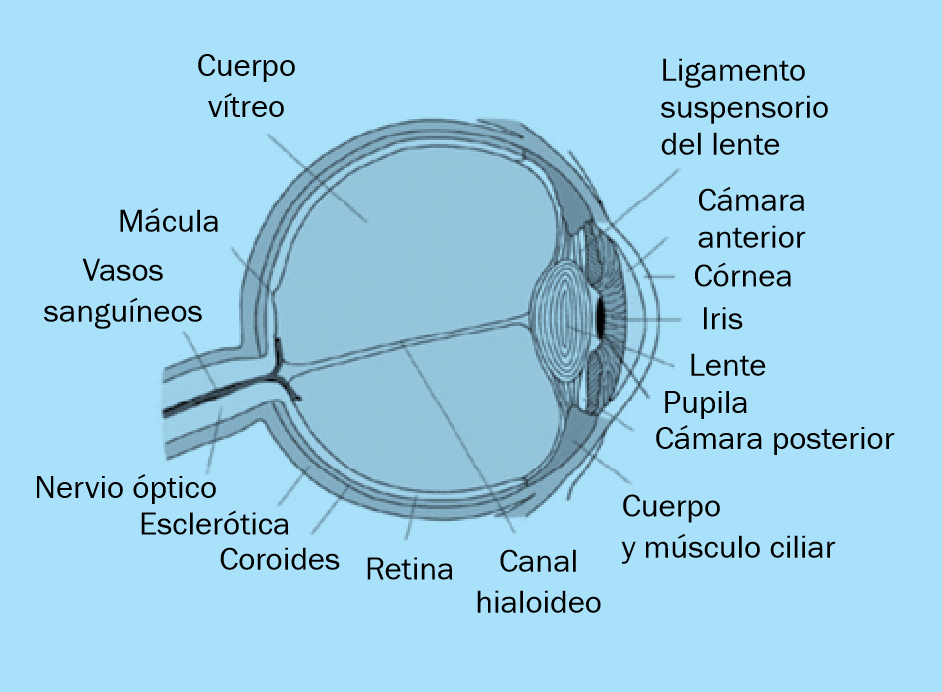
\includegraphics[width=0.45\textwidth]{imaxes/ojo1.png}
    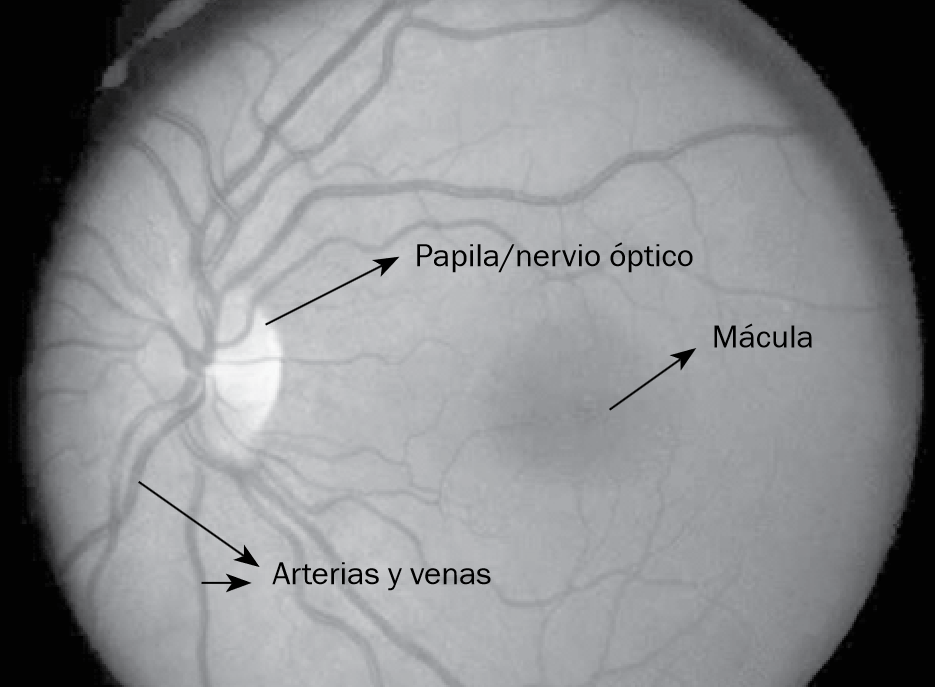
\includegraphics[width=0.45\textwidth]{imaxes/ojo2.png}
    \caption{Imaxes do ollo humano, extraídas de \cite{visionyojo}. Á esquerda, vista lateral do ollo anotada. Á dereita, retinografía do ollo anotada.}
    \label{fig:imaxes_ojo}
\end{figure}

\subsection{Imaxe oftalmolóxica}
\label{subsec:Imaxe oftalmolóxica}
Existen diversas modalidades de imaxe médica que permiten observar o ollo, cada unha con diferentes propiedades e aplicacións. 
Entre elas inclúense a fotografía de fondo de ollo, a tomografía de coherencia óptica (OCT) e a angiografía con fluoresceína \cite{ilginis2014ophthalmic}.

Este traballo céntrase na fotografía de fondo de ollo entre outras razóns polo seu uso común na práctica clínica.
Isto é débese en gran parte á súa accesibilidade, requerindo equipo máipólas barato e menor adestramento comparada cas outras modalidades. 
Ademais, é unha técnica non invasiva e rápida de realizar, o que a fai preferible na maioría dos casos \cite{retinimaging}.

Para realizala faise uso dunha cámara especial denominada retinógrafo, e xeralmente require da previa dilatación da pupila do paciente.
Desta forma permítese maior entrada de luz nos ollos, o que provoca unha mellor visualización da retina e mellora a calidade da imaxe.
Un especialista pode analizar a retinografía para detectar signos de enfermidades como a retinopatía diabética, a hipertensión ou a dexeneración macular \cite{retreggood}.

\section{Rexistro de imaxes}
\label{sec:Rexistro de imaxes}
O rexistro de imaxes é un proceso que consiste en, sobre dúas ou máis imaxes, determinar a correspondencia espacial entre elas
 e alinealas nun sistema de coordenadas común, co obxetivo de que as características de interese se atopen na mesma posición.

% Por exemplo, no caso do stitching de fotografías panorámicas, o rexistro de imaxes permite identificar correspondencias entre puntos característicos en múltiples tomas solapadas
%  e axustar a súa posición relativa nun marco común. Esta etapa é necesaria para a posterior fusión das imaxes, de modo que as distintas vistas se aliñen con precisión, producindo un resultado final continuo e sen irregularidades visuais.

O rexistro de imaxes ten utilidade en moitos campos diferentes como a imaxe satelital, xeografía, robótica... mais o 
campo da imaxe médica é dos máis interesantes pola súa aplicación práctica e é o que se aborda neste traballo \cite{goshtasby2017theory}.
Estas imaxes poden variar a nivel temporal, espacial, de dimensión ou de modalidade.

No ámbito da saúde un rexistro adecuado pode empregarse para comparar imaxes dun mesmo paciente tomadas en distintos momentos, en distintas modalidades ou para comparar entre diferentes pacientes.
Isto permite a revisión do avance dunha enfermidade ao longo do tempo, a fusión de imaxes de distintas modalidades ou a detección de patróns comúns entre distintos individuos.
A fusión de imaxes permite interpretar moito mellor a información dispoñible nelas, e é de gran axuda para guiar aos médicos na toma de decisións.
Tamén é útil para correxir os movementos involuntarios do paciente durante a adquisición de imaxes, como no caso da respiración en imaxes de pulmóns, ou para a intervención guiada por imaxe (\gls{IGRT}) que non 
podería funcionar sen a utilización axeitada de técnicas de rexistro de imaxes \cite{wang2022neuralrenderingstereo3d}. 

Ata recentemente, gran parte do traballo de rexistro facíase de forma manual por expertos con software como BigWarp \cite{bigwarp}, 
e dependía das habilidades do profesional para detectar as características de interese e realizar o aliñamento.
Isto facía que o proceso fose lento e propenso a erros, ademais de pouco práctico para grandes volumes de imaxes.

Na figura \ref{fig:retin_reg} móstrase un exemplo de rexistro de imaxes de retina, onde se pode observar como as imaxes son aliñadas para que as estruturas anatómicas coincidan.

\begin{figure}[tbp]
    \centering
    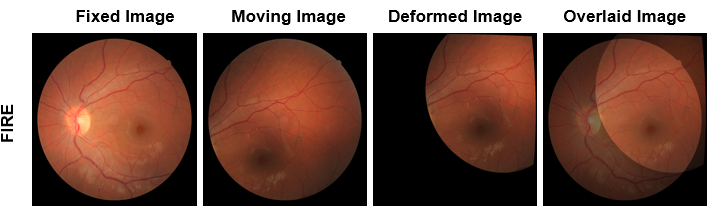
\includegraphics[width=0.8\textwidth]{imaxes/retin-reg.png}
    \caption{Exemplo de rexistro de imaxes de retina \cite{sivaraman2024retinaregnetzeroshotapproachretinal}}
    \label{fig:retin_reg}
\end{figure}

\subsection{Categorías de rexistro}
\label{subsec:Categorías de rexistro}

% O rexistro de imaxes pode ser clasificado en distintas categorías segundo as súas características. Na figura \ref{fig:categorias_de_rexistro} un resumo móstranse das categorías mais comúns.
O rexistro de imaxes pode ser clasificado en distintas categorías segundo as súas características.
% \begin{figure}[hp!]
%     \centering
%     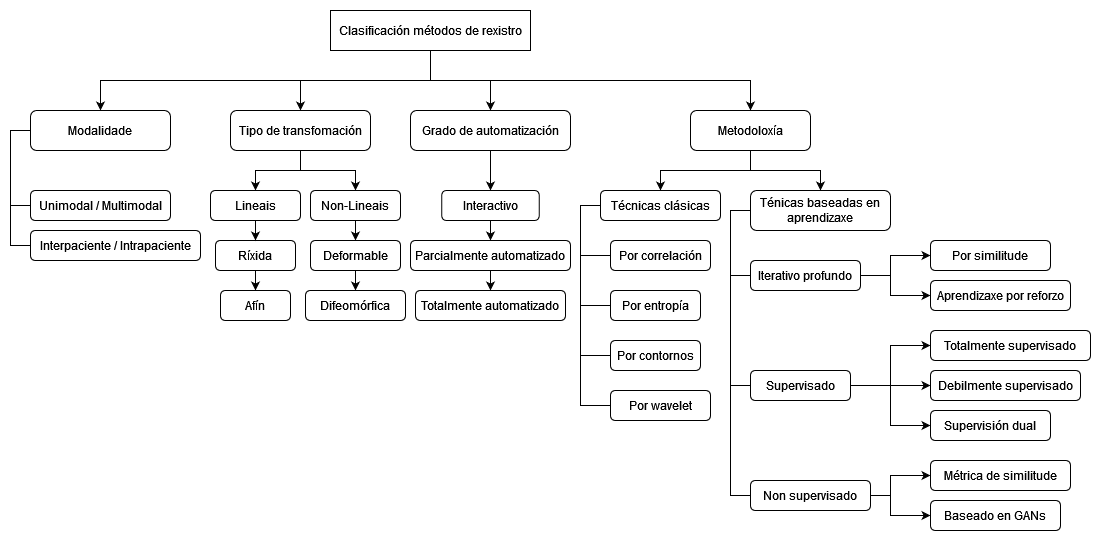
\includegraphics[width=1\textwidth]{imaxes/catreg.drawio.png}
%     \caption{Categorías de rexistro}
%     \label{fig:categorias_de_rexistro}
% \end{figure}

\begin{itemize}
    \item \textbf{Segundo o número de imaxes:}
    \begin{itemize}
        \item \textit{Par a par:} O rexistro realízase entre dúas imaxes, unha fixa e unha móbil.
        \item \textit{Múltiple:} Rexístranse varias imaxes simultaneamente, buscando unha correspondencia global.
    \end{itemize}

    \item \textbf{Segundo a modalidade:}
    \begin{itemize}
        \item \textit{Intra-modalidade:} As imaxes pertencen á mesma modalidade (por exemplo, dúas retinografías).
        \item \textit{Inter-modalidade:} As imaxes proveñen de modalidades diferentes (por exemplo, retinografía e OCT).
    \end{itemize}

    \item \textbf{Segundo o tipo de transformación:}
    \begin{itemize}
        \item \textit{Ríxida:} Só permite traslación e rotación, mantendo as distancias e ángulos.
        \item \textit{Afín:} Ademais de traslación e rotación, permite escalado e cizallamento.
        \item \textit{Deformable (non ríxida):} Permite deformacións locais complexas e non lineais.
        \item \textit{Difeomórfica:} Transformación non ríxida que é continua, invertible e diferenciable en todo o seu dominio. Se non ten esta característica, non se pode garantir que a transformación sexa reversíbel, polo que son preferidas en moitos casos \cite{han2022diffeomorphicimageregistrationneural}.
    \end{itemize}

    \item \textbf{Segundo o grao de automatización:} \cite{deeplernreview3dreg}
    \begin{itemize}
        \item \textit{Manual:} O usuario selecciona puntos de control ou axusta parámetros.
        \item \textit{Automático:} O proceso realízase sen intervención humana, mediante algoritmos.
        \item \textit{Semiautomático:} Combina intervención manual e automática.
    \end{itemize}

    \item \textbf{Segundo a natureza da transformación:}
    \begin{itemize}
        \item \textit{Simétrico:} A transformación é consistente en ambas direccións entre as imaxes.
        \item \textit{Asimétrico:} A transformación calcúlase só nun sentido. Cando se traballa con imaxes de forma asimétrica, a imaxe de referencia denomínase imaxe fixa e a imaxe que se quere rexistrar imaxe móbil.
    \end{itemize}

\end{itemize}

% \begin{itemize}
%     \item \textbf{Metodoloxía}
%     \begin{itemize}
%         \item \textbf{Técnicas clásicas} \cite{zitova2003imageregistrationsurvey}
%         \begin{itemize}
%             \item \textit{Por correlación:} Optimizan funcións de correlación entre as intensidades das imaxes para atopar a mellor aliñación.
%             \item \textit{Por entropía:} Baseados na maximización da información mutua, resultan especialmente útiles en rexistro multimodal.
%             \item \textit{Por contornos:} Empregan características xeométricas, como bordes ou liñas estruturais, para establecer correspondencias espaciais.
%             \item \textit{Por wavelet:} Utilizan descomposicións en diferentes frecuencias e resolucións para capturar información relevante.
%         \end{itemize}
        
%         \item \textbf{Técnicas baseadas en aprendizaxe} \cite{deeplernreview3dreg, bharati2022deeplearningmedicalimage}
%         \begin{itemize}
%             \item \textit{Iterativo profundo:} Estratexias que aplican redes neurais de forma recursiva para refinar progresivamente a transformación estimada.
            
%             \item \textbf{Aprendizaxe supervisada}
%             \begin{itemize}
%                 \item \textit{Totalmente supervisado:} Require datos de adestramento con aliñacións precisas (ground truth), que permiten optimizar directamente a tarefa de rexistro.
%                 \item \textit{Debilmente supervisado:} Emprega información parcial ou indirecta, como anotacións espaciais limitadas ou métricas proxy.
%                 \item \textit{Supervisión dual:} Combina diferentes formas de supervisión, como etiquetas explícitas e funcións de perda auto-supervisadas, para aumentar a xeneralización.
%             \end{itemize}
            
%             \item \textbf{Aprendizaxe non supervisada}
%             \begin{itemize}
%                 \item \textit{Métrica de similitude:} Optimiza criterios de similitude (e.g., NCC, SSIM) sen necesidade de datos anotados, favorecendo adaptación a novos dominios.
%                 \item \textit{Baseado en GANs:} Emprega arquitecturas adversarias para aprender transformacións realistas entre imaxes sen supervisión directa.
%             \end{itemize}
            
%             \item \textit{Por similitude:} Modelos que aprenden funcións de custo diferenciables que maximizan a coincidencia entre as imaxes de entrada.
%             \item \textit{Aprendizaxe por reforzo:} Formula o rexistro como un problema de toma de decisións, onde un axente aprende políticas óptimas mediante retroalimentación ambiental.
%         \end{itemize}
%     \end{itemize}
% \end{itemize}

As transformacións lineais globais soen representanse en matrices de transformación, onde cada elemento da matriz representa un parámetro da transformación.

No caso de transformacións máis complexas, utilízanse campos de vectores de deformación (\gls{DFV}s), que permite representar deformacións locais na imaxe, facendoa moito máis flexible para representar transformacións non lineais e detalladas.
Os DFVs adoitan ser representados cunha matriz de igual tamaño á imaxe, onde cada elemento representa un vector que indica a dirección e a magnitude da deformación.

Este traballo ubícase no rexistro de imaxes par a par, intra-modaliade e con transformacións deformables. É un proceso totalmente automático que produce transfomacións asimétricas.

Na figura \ref{fig:dfv_visualization} móstranse dúas formas de visualizar un DFV: mediante frechas que indican a dirección e magnitude da deformación, e aplicando a deformación a unha cuadrícula para ver como se distorsiona.

\begin{figure}[tbp]
    \centering
    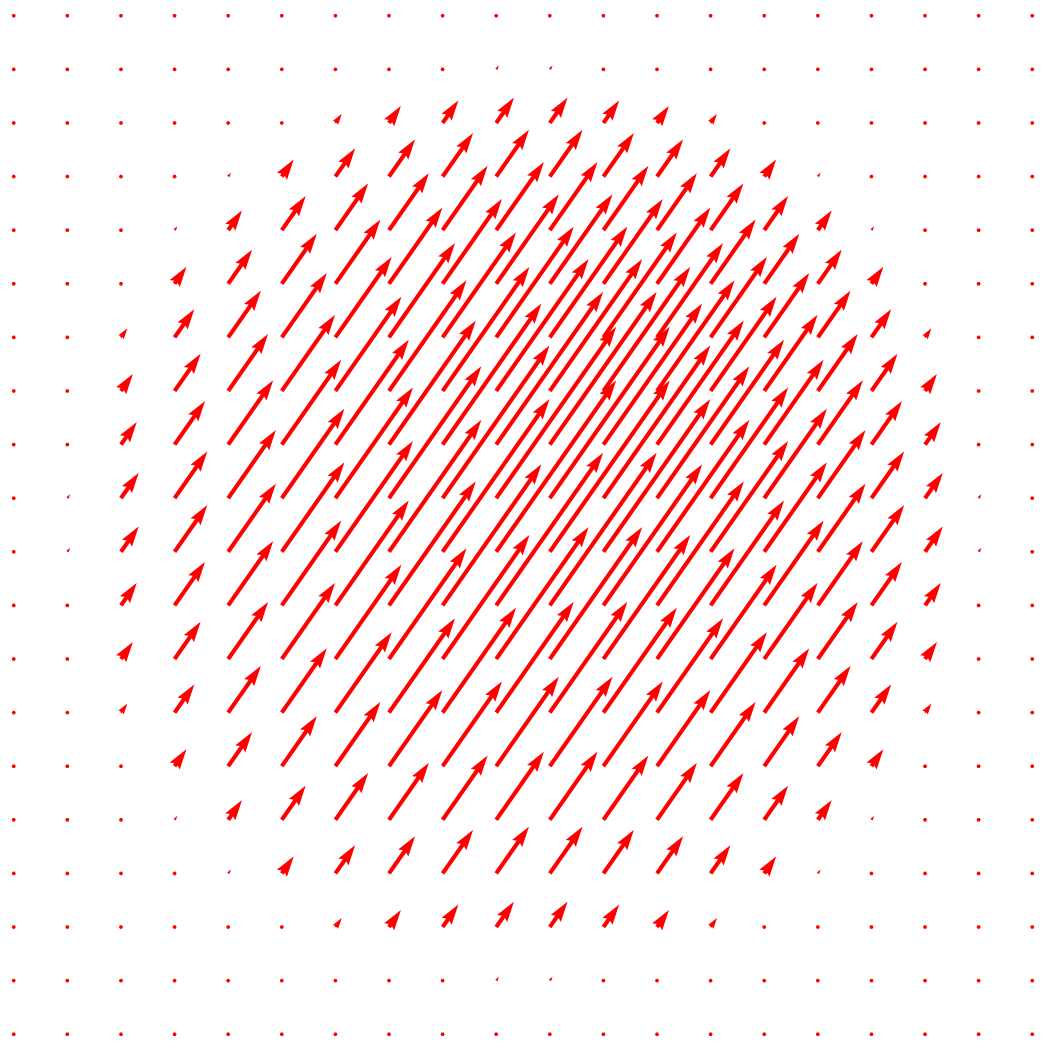
\includegraphics[width=0.45\textwidth]{imaxes/dfv_arrows.png}
    
\includegraphics[width=0.45\textwidth]{imaxes/dfv_grid.png}
    \caption{Visualización do campo de vectores de deformación (DFV). Á esquerda, representación mediante frechas. Á dereita, esta deformación aplicada a unha cuadrícula.}
    \label{fig:dfv_visualization}
\end{figure}

\subsection{Estado da arte}
\label{subsec:Estado da arte}

% Pese á gran cantidade de avances que está a ocorren no campo do aprendizaxe profunda, os métodos clásicos de rexistro de imaxes seguen a ser o estado do arte na maioría de casos,
% principalmente debido á importancia da precisión e a robustez en imaxe médica.

O rexistro de imaxes médicas constitúe unha área de investigación fundamental que experimentou importantes avances nas últimas décadas. Neste ámbito, a precisión e a robustez do rexistro cobran especial relevancia, xa que son empregados para o diagnóstico e seguimento de enfermidades, así como para a planificación de tratamentos cirúrxicos.
No eido da oftalmoloxía, os métodos que funcionan ben en varios dominios de imaxe médica (cerebro, pulmóns, etc) adoitan requirir de axustes para funcionar en retinas, polo que hai un estado da arte paralelo. 

A evolución dos métodos de rexistro en retinografías reflicte a transición dende enfoques puramente algorítmicos cara metodoloxías híbridas, onde publicacións recentes como HybridRetina \cite{liu2024progressiveretinalimageregistration}  mostran como para acadar os mellores resultados é beneficioso combinar ambos enfoques, aproveitando a precisión dos métodos clásicos e a adaptabilidade dos métodos de aprendizaxe automático.

\subsubsection{Métodos clásicos}
\label{subsubsec:Métodos clásicos}

Os métodos clásicos de rexistro de imaxes médicas poden clasificarse en dúas categorías principais:
Aqueles baseados en similitude de imaxe (\gls{IBR}) e aqueles baseados en características (\gls{FBR}).
Tamén existen métodos híbridos que combinan ambos enfoques \cite{integrateintfeat}.
O resultado final pode ser os parámetros da transformación ou a imaxe fusionada.

\paragraph{Métodos baseados en similitude de imaxe}
\label{par:Métodos baseados en similitude de imaxe}

O rexistro realízase comparando os valores de intensidade dos píxeles ou voxeles mediante unha métrica de similitude entre a imaxe fixa e a imaxe móbil.
Este enfoque tende a requerir de múltiples iteracións para converxer, nas cales calcúlase o grado de semellanza entre as imaxes e
actualízanse os parámetros da transformación utilizando un mecanismo de optimización ata que se cumpran os criterios de terminación.

Os métodos de rexistro tradicionais teñen tres compoñentes principais: a métrica de similitude, o optimizador e o modelo de transformación. 

A figura \ref{fig:rexistro_iterativo} mostra un diagrama do proceso de rexistro iterativo.

% ejemplos?

\paragraph{Métodos baseados en características}
\label{par:Métodos baseados en características}

O rexistro realízase identificando e emparellando características salientables entre as imaxes, como puntos, liñas ou bordes.
Tipicamente, estes métodos teñen 3 pasos principais:

\begin{itemize}
\item \textbf{Detección de puntos de interese:} Identificación de puntos ou rexións salientables nas imaxes, como bordes, esquinas ou texturas. Para isto poden utilizarse utilízanse algoritmos como SIFT \cite{sift}, SURF \cite{surf}, BRISK \cite{brisk} ou FREAK \cite{freakkeypoint}.
\item \textbf{Descrición de características:}  os puntos detectados son descritos e comparados entre imaxes usando descritores .
\item \textbf{Estimación da transformación:} unha vez atopadas as correspondencias, calcúlase a transformación que aliña as imaxes con algoritmos de emparellamento como FLANN \cite{flann} ou RANSAC \cite{ransac}.
\end{itemize}

Algúns dos métodos tradicionalmente máis utilizados neste campo son \gls{GDB-ICP} \cite{GDB-ICP} e Harris-PIIFD \cite{piifd}. Este último utiliza o algoritmo Harris \cite{Harris1988ACC} para a detección de puntos de interese, descríbenos con \gls{PIIFD}, e emparéllanse usando \gls{BBF} \cite{BBF}.
 Finalmente, refínanse as coincidencias e escóllese a transformación (ríxida, afín ou polinomial) segundo o número de pares de puntos válidos. Sobre esta base propuxéronse varias melloras para adaptalo ao rexistro multimodal de retinas como UR-SIFT \cite{ur-sift} ou \gls{GMM} \cite{GMM}.

Unha vantaxe deste enfoque é a capacidade para rexistrar imaxes con grandes variacións locais ou modalidades diferentes, xa que non depende tanto da semellanza global entre as imaxes.

Outros métodos clásicos relevantes no campo da imaxe de ollo inclúen REMPE \cite{rempe}, que estima simultaneamente a pose das cámaras e a forma do ollo. Fai uso de un modelo elipsoidal para o ollo e estima a posición das cámaras con RANSAC, para logo refinala cunha variante de PSO \cite{pso}. 
% Versións anteriores deste método utilizaron modelos esféricos e \gls{SURF} no canto de SIFT \cite{H-M16}.

\begin{figure}[tbp]
\centering
\begin{tikzpicture}[node distance=2cm, scale=0.8, every node/.style={transform shape}]
% Nodes
\node (imageFixa) [process] {Imaxe Fixa};
\node (imageMobil) [process, right of=imageFixa, xshift=3cm] {Imaxe Móbil};
\node (featureExtraction) [process, below of=imageFixa, yshift=-1cm] {Cálculo de medida de similitude};
\node (parameterUpdate) [process, below of=featureExtraction, yshift=-1cm] {Actualización de Parámetros};
\node (applyTransformation) [process, below of=parameterUpdate, yshift=-1cm] {Aplicar a Transformación};
\node (criteriaCheck) [decision, below of=applyTransformation, yshift=-1cm] {Criterios Cumpridos?};
\node (result) [process, below of=criteriaCheck, yshift=-1cm] {Resultado};
% Arrows
\draw [arrow] (imageFixa) -- (featureExtraction);
\draw [arrow] (imageMobil) -- (featureExtraction);
\draw [arrow] (featureExtraction) -- (parameterUpdate);
\draw [arrow] (parameterUpdate) -- (applyTransformation);
\draw [arrow] (applyTransformation) -- (criteriaCheck);
\draw [arrow] (criteriaCheck) -- node[anchor=west] {Sí} (result);
\draw [arrow] (criteriaCheck.east) -- ++(1,0) node[anchor=south, xshift=0.5cm] {No} |- (featureExtraction.east);
\end{tikzpicture}
\caption{Proceso de rexistro de imaxes iterativo}
\label{fig:rexistro_iterativo}
\end{figure}

Tamén existen múltiples programas que fan uso de estos métodos en ferramentas para facilitar o rexistro de imaxes, como SimpleITK \cite{simpleitk}, Elastix \cite{elastix} ou ANTs \cite{ants}.

\subsubsection{Métodos de aprendizaxe profunda}
\label{subsubsec:Métodos de aprendizaxe profunda}

Coa chegada dos métodos de aprendizaxe profunda á imaxe médica, comezaron a empregarse redes neuronais para realizar o aliñamento de imaxes.
Existe un gran interés polos métodos baseados en aprendizaxe profundo, como se reflexa no crecente número de publicacións no campo. Na figura \ref{fig:method_comp} móstrase a evolución do número de publicacións sobre rexistro de imaxes, diferenciando entre os métodos baseados en aprendizaxe profunda e os métodos tradicionais.

% Estos métodos tenden a ser mais rápidos que os métodos convencionais, a custo de algo de precisión.
Os métodos de aprendizaxe profunda poden ser clasificados en dous tipos según se requiran de \glossary{DFV}s anotados ou non na etapa de adestramento:
supervisados (requíren anotacións) e non supervisados (non requíren anotacións) \cite{nie2024medicalimageregistrationapplication}.

Segundo o grado de supervisión utilizado na etapa de adestramento, os métodos supervisados poden dividirse en supervisados ou débilmente supervisados.
O rexistro totalmente supervisado fai uso de DVFs de referencia para supervisar o proceso de aprendizaxe, e o termo de perda adoita basearse na discrepancia entre os DVFs de referencia e os DVFs predicidos.

O rexistro débilmente supervisado pode utilizar outras etiquetas de referencia implícitas, non baseadas en datos explícitos como os DFVs, senón que utilizan información indirecta para guiar o proceso de rexistro, como a semellanza entre as imaxes ou restricións baseadas na forma ou límites anatómicos das estruturas.
Máis de dous tipos de datos de referencia son frecuentemente utilizados para adestrar modelos de rexistro débilmente supervisados \cite{bharati2022deeplearningmedicalimage}.

Os métodos non supervisados teñen a vantaxe de non requirir de datos anotados, o cal é unha gran vantaxe xa que un dos maiores retos para as redes de imaxes médicas é a recolección de datos de calidade para o adestramento \cite{medicalimageanalysis}.
A creación de conxuntos de DFVs anotados é un proceso laborioso e costoso, que normalmente sólo póde ser executado por especialistas, polo que os métodos de rexistro non supervisados son de gran interese.
De forma similar aos métodos iterativos, é común empregar unha métrica de similitude entre as imaxes xunto con un termo de regularización para guiar o proceso de optimización evitando caer en transformación non realistas.
% Xa que a imaxe fixa e a imaxe móbil xa conteñen toda a información necesaria para un rexistro correcto, os métodos non supervisados parecen mais adecuados para a tarefa de rexistro.

Os enfoques de aprendizaxe profundo son útiles tanto na súa capacidade de aprender a tarefa de rexistro de maneira end-to-end, como para substituír módulos concretos do proceso tradicional.
Nese sentido, os métodos de aprendizaxe profunda poden ser categorizados según a tarefa do proceso de rexistro que substitúen.

\begin{figure}[tbp]
\centering
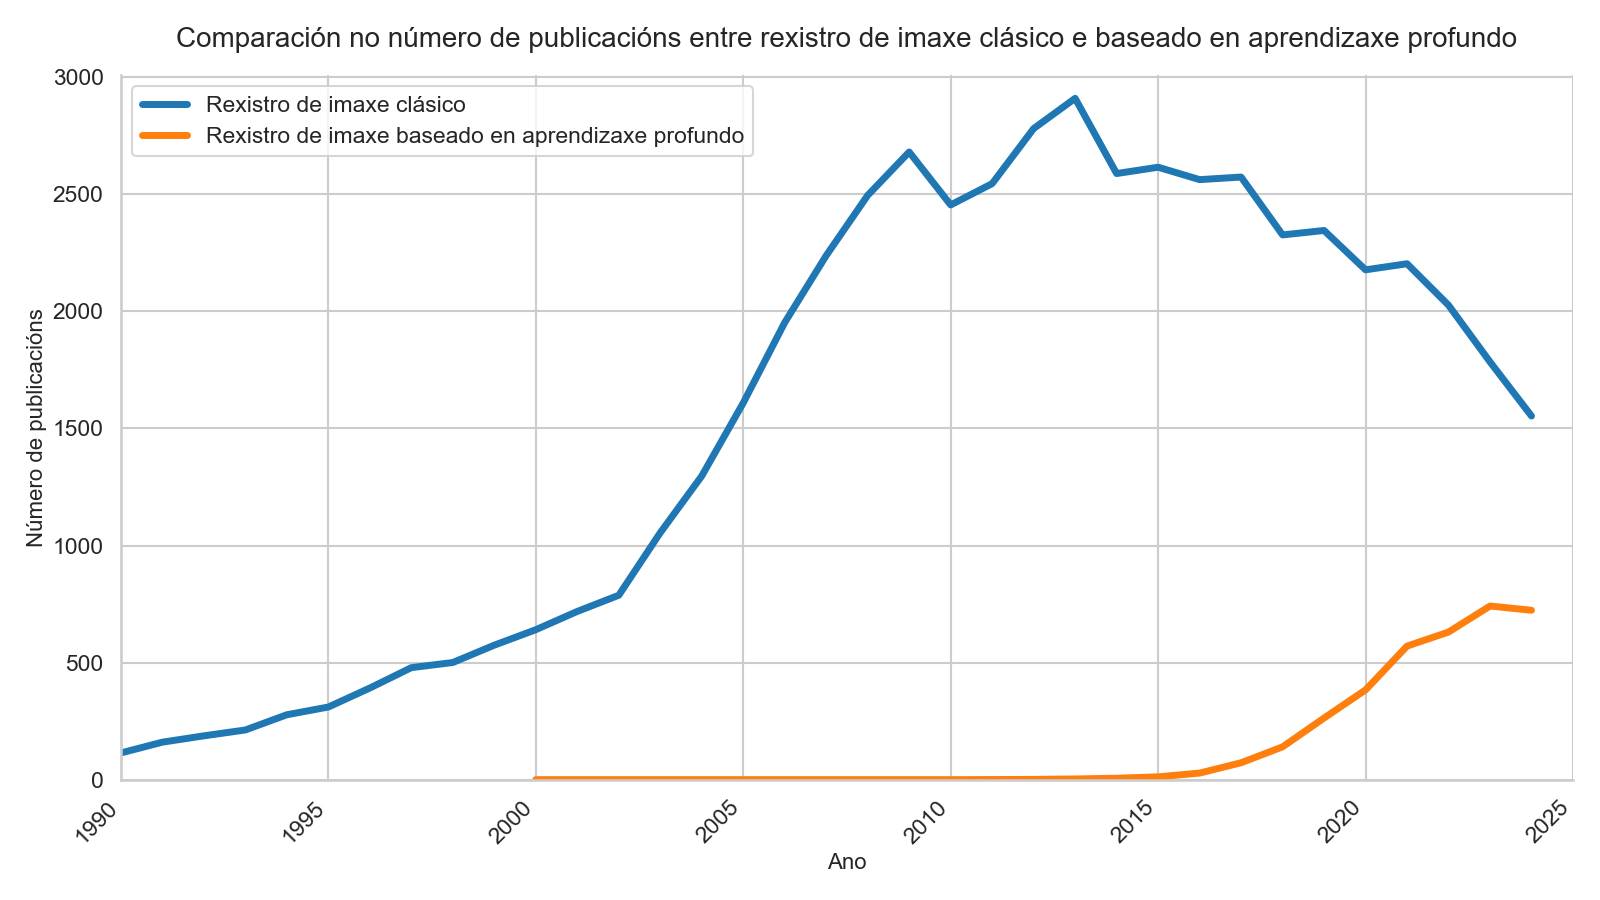
\includegraphics[width=0.8\textwidth]{imaxes/methods_comp.png}
\caption{Comparación de pubicacións ó longo do tempo que relacionadas co rexistro de imaxes. Datos extraídos de Scopus \cite{scopus}, realizando as consultas: "TITLE-ABS-KEY(image AND registration) AND NOT(deep AND learning)" e "TITLE-ABS-KEY(image AND registration) AND (deep AND learning)"}
\label{fig:method_comp}
\end{figure}

Os métodos de aprendizaxe profunda poden substituír calquera destes pasos que forman os métodos de rexistro clásicos de forma independente ou en combinación.

\paragraph{En rexistro baseado en intensidade (IBR)}
\label{par:IBR_substitution}

\begin{itemize}
\item \textbf{Métrica de similitude:} Os métodos de aprendizaxe profunda poden aprender métricas de similitude máis robustas que as tradicionais. Estas métricas aprendidas poden ser máis efectivas en imaxes multimodais ou con artefactos.
Por exemplo, Czolbe et al. \cite{semanticsimilarity} propoñen dúas métricas de similitude semánticas que aprende a semellanza entre imaxes comparando as características de alto nivel extraídas. Presentan unha aproximación non supervisada que fai uso de autoencoders e outra semisupervisada que incorpora datos de segmentación.
\item \textbf{Optimizador:} Os métodos de aprendizaxe profunda poden substituír o proceso de optimización iterativa tradicional por redes que aprenden a predicir directamente os parámetros de transformación óptimos. Unha aproximación común é empregar estes conxuntos de datos para optimizar unha CNN que, dadas dúas imaxes novas e non vistas, predí o DFV correspondente \cite{defregcnn}. Durante o proceso de adestramento, a rede pode ter acceso aos DFVs coa deformación correcta, ou pódense obter indirectamente a través da optimización dunha métrica de similitude de imaxes.
\item \textbf{Modelo de transformación:} Estes métodos aprenden representacións implícitas da transformación a través de redes neuronais, permitindo modelar deformacións máis complexas que os modelos paramétricos tradicionais. Os métodos como IDIR \cite{wolterink2021implicit} encaixan nesta categoría, utilizando campos neuronais implícitos para representar as transformacións de rexistro.
\end{itemize}

% Existen diferentes extensións a esta aproximación, como o uso de múltiples etapas ou o uso de redes adversarias durante o adestramento.

% Tamén se propuxeron métodos híbridos que combinan a optimización iterativa ca aprendizaxe profunda,
% entrenando unha CNN nova por cada parella de imaxes. Desta forma conséguese evitar a necesidade de grandes conxuntos de datos para o adestramento.

\paragraph{En rexistro baseado en características (FBR)}
\label{par:FBR_substitution}

\begin{itemize}
\item \textbf{Detectores de características:} As redes neuronais poden aprender a detectar puntos de interese máis robustos e repetibles que os detectores clásicos como \glossary{SIFT}. SuperPoint \cite{superpoint} introduce un detector de características baseado en redes neuronais que aprende a detectar puntos de interese e a describilos simultaneamente.
\item \textbf{Descriptores de características:} Os descriptores aprendidos mediante redes neuronais poden capturar información máis discriminativa, mellorando a precisión do emparellamento posterior. Estes métodos aprenden representacións que son invariantes a transformacións específicas do dominio.
\item \textbf{Emparellamento:} As redes neuronais poden aprender a realizar o emparellamento de características de forma robusta, especialmente en presenza de cambios de iluminación ou perspectiva. SuperGlue \cite{superglue} é un exemplo de modelo que aprende a emparellar puntos de interese detectados utilizando unha arquitectura baseada en atención para capturar as relacións entre os puntos.
\end{itemize}

\paragraph{Métodos de regresión directa}
\label{par:direct_regression}

A aprendizaxe profunda tenden a requerir dunha gran cantidade de datos para ser adestrados, o que pode ser unha desventaxa xa que en moitos casos non se dispoñen de bases de datos anotadas do tamaño necesario.

Os métodos de regresión directa aprenden a mapear directamente desde un par de imaxes ata os parámetros da transformación, sen necesidade de optimización iterativa nin extracción explícita de características.

Tamén son denominados métodos de inferencia amortizada debido á capacidade de realizar múltiples inferencias (rexistros) tras un único proceso de adestramento, en contraposición aos métodos tradicionais que requiren optimización individual para cada par de imaxes.
Estes enfoques son útiles pola súa eficiencia computacional na fase de inferencia. Voxelmorph \cite{Balakrishnan_2019voxelmorph} é un dos frameworks máis utilizados no rexistro de imaxes deformable, facendo uso de modelos baseado en \gls{CNN}s e que tamén permite incorporar información auxiliar (como segmentacións) se está dispoñible, mellorando así a precisión do rexistro.

Métodos como UDIR-Net \cite{undefreg} ou DIO \cite{Jena_2025} tamén implementan estas ideas.

% \paragraph{GANs}
% \label{par:GANs}

% As \gls{GAN} (Generative Adversarial Network) son un tipo de rede neuronal que consta de dous modelos que compiten entre si: un xerador e un discriminador. O xerador intenta crear datos falsos que sexan indistinguibles dos datos reais, mentres que o discriminador intenta distinguir entre os datos reais e os datos xerados. Este proceso de competición mellora iterativamente a calidade dos datos xerados e o criterio do discriminador.

% No contexto do rexistro de imaxes, as GANs poden ser utilizadas para aprender a transformación entre imaxes de forma non supervisada. O xerador pode ser adestrado para producir transformacións que aliñen a imaxe móbil coa imaxe fixa, mentres que o discriminador avalía a calidade do rexistro.
% Un exemplo de aplicación de GANs no rexistro de imaxes médicas é o traballo de Mahapatra et al. \cite{mahapatra2019ganbasedmedicalimage}, onde se propón un modelo de rexistro de imaxes baseado en GANs que demostrou ser efectivo tanto en retinas como con resonancias magnéticas cardiovasculares.

\subsubsection{Estado da arte no rexistro de retinografías}
\label{subsubsec:Estado_da_arte_no_rexistro_de_retinografías}

O rexistro de retinografías presenta un conxunto de desafíos únicos que o distinguen doutros dominios da imaxe médica.
Un dos principais obstáculos son as deformacións non ríxidas. Estas deformacións poden orixínarse pola proxección da superficie 3D curva da retina nunha imaxe 2D ou variacións na forma do ollo de cada paciente. Ademais, é frecuente atopar pares de imaxes con áreas de solapamento mínimas o que dificulta a identificación de correspondencias para o aliñamento. A isto súmanse as variacións de iluminación, contraste e cor entre imaxes capturadas en diferentes situacións, así como os cambios anatómicos inducidos por patoloxías, que alteran as estruturas utilizadas para o rexistro. 
Finalmente, a escaseza de conxuntos de datos públicos, especialmente para condicións ou poboacións específicas, supón unha barreira importante para o desenvolvemento de modelos de aprendizaxe supervisada.    

A dificultade para obter campos de deformación de referencia para o adestramento impulsou o desenvolvemento de marcos non supervisados. Estes modelos adéstranse optimizando unha función de perda baseada na similitude de imaxe entre a imaxe móbil deformada e a imaxe fixa, xunto cun termo de regularización sobre a suavidade da deformación. 

% A figura \ref{tab:retina_reg_comp} mostra unha análise comparativa revela un claro compromiso entre precisión e velocidade. Métodos clásicos como REMPE poden acadar unha alta precisión, pero son computacionalmente moi custosos (p. ex., 198 segundos por par de imaxes). En contraste, os métodos de aprendizaxe profunda son ordes de magnitude máis rápidos (p. ex., 0.65 segundos por par), aínda que poden sacrificar parte da precisión nos casos máis complexos. A seguinte táboa resume esta comparativa.  

Dentro dos métodos clásicos, os baseados en características (FBR) seguen a ser referentes en canto a precisión. Entre eles destacan VOTUS \cite{Votus}, que é especialmente robusto en imaxes de pouco solapamento e representa as árbores vasculares como grafos para atopar a correspondencia entre eles. REMPE \cite{rempe} é outro método xa mencionado anteriormente nesta categoría.

No campo da aprendizaxe profunda, RetinaRegNet \cite{sivaraman2024retinaregnetzeroshotapproachretinal} é un modelo recente que de tipo "zero-shot" que utiliza características extraídas de modelos de difusión para establecer correspondencias, acadando resultados de vangarda

%  \cite{ConKeD}  \cite{ConKeD2}
ConKeD (Contrastive Keypoint Descriptors) e a súa evolución, ConKeD++ , céntranse en perfeccionar a creación de descritores de puntos de interese, un dos compoñentes máis críticos dos métodos baseados en características (FBR).
A principal vantaxe é que obtén resultados comparables aos dos métodos clásicos de vangarda (como REMPE e VOTUS) pero con tempos de execución moito máis rápidos

A maioría destes algoritmos son avaliados e comparados utilizando o conxunto de datos de referencia FIRE \cite{FIRE}, permitindo unha cuantificación obxectiva do rendemento.

\section{Representación Neuronais Implícitas}
\label{sec:Representación Neuronais Implícitas} 

A representación de coñecemento é un dos problemas máis importantes na área da computación, e as 
redes profundas son unha das ferramentas máis útiles, especialmente no campo da visión por computador.
Tradicionalmente empréganse representacións discretas, onde o espazo de entrada é dividido en celdas e cada celda é asignada un valor (por exemplo nubes de puntos, matrices de píxeles ou vóxeles...).
Unha das principais desventaxas destas representacións é que a súa complexidade increméntase rápidamente co número de dimensións representadas, ademais do custo de memoria asociado.

 As representacións neuronais implícitas son un paradigma innovador que permite modelar sinais continuas mediante funcións parametrizadas por redes neuronales.
 Codifican a información como unha función continua, que mapea valores de entrada aos valores correspondientes de saída, en lugar de almacenar directamente valores de características o señales.

Representar o sinal como una función continua permite solucionar os problemas asociados á discretización e obtéñense outra serie de vantaxes.

As INR son moito mais eficientes debido á compresión da información que realizan de forma implícita. Ao mesmo tempo, permite un nivel de detalle non limitado pola resolución da imaxe, senón pola capacidade da rede. 
 Ademais, as representacións continuas son diferenciables, o que permite o cálculo de gradientes e derivadas de forma analítica en lugar de ter que aproximalos por diferencias finitas.
 Isto tamén implica que as representacións implícitas son independentes da resolución, o que permite a reconstrucción en calquera escala espacial.
 
Tipicamente emprégase un MLP como architectura para representar a función implícita. Non obstante, o uso da función de activación ReLU tende a non obter os mellores resultados, debido a que son incapaces de representar deformacións locais sen afectar o sea comportamento global \cite{rahaman2019spectralbiasneuralnetworks},
polo que moita investigación diríxese a atopar alternativas que melloren a representación do sinal. \cite{essakine2024standimplicitneuralrepresentations}

Unha destas alternativas é SIREN \cite{sitzmann2020implicitneuralrepresentationsperiodic}, sobre a que profundizaremos máis adiante.
Outras propostas inclúen \cite{ramasinghe2022periodicityunifyingframeworkactivations} propón as funcións de activación gaussianas como alternativa a SIREN, e argumenta que poden obter mellores representacións e máis robustas.
\cite{saragadam2023wirewaveletimplicitneural} achega unha nova función de activación baseada en wavelets, que parece ser especialmente útil para a representación de imaxes.

As representacións implícitas poden ser clasificadas en dúas categorías: xeneralizables e sobreaxustadas \cite{yu2024neuraltrajectorymodelimplicit}. 
As representacións sobreaxustadas céntranse en reproducir con precisión unha única sinal, mentres que as representacións xeneralizables poden modelar varias nunha mesma rede.

\subsection{Aplicacións}
\label{subsec:Aplicacións}

As INR son utilizadas en todo tipo de campos, dende xeración de imaxes \cite{reddy2022multiimplicitneuralrepresentationfonts}, pasando por
reconstrucción de obxetos \cite{mildenhall2020nerfrepresentingscenesneural} \cite{mescheder2019occupancynetworkslearning3d} ou modelado de sinais complexas \cite{wu2021iremhighresolutionmagneticresonance}.

As representacións implícitas están a recibir cada vez máis atención da comunidade médica, e son 
especialmente útiles para as tarefas de imaxe inversa, que requiren a reconstrucción de representacións correctas a partir de datos incompletos ou ruidosos \cite{molaei2023implicitneuralrepresentationmedical}. 
Métodos como NeRP, propuxeron o uso de representacións implícitas para a reconstrucción de imaxes de resonancia magnética a partir de datos incompletos, 
e obtiveron resultados comparables a métodos tradicionais \cite{shen2023nerpimplicitneuralrepresentation}.

NeRF fai uso de representacións implícitas para a sintetizar novos puntos de vista en escenas 3D  \cite{mildenhall2020nerfrepresentingscenesneural}, 
 optimizando unha función volumétrica continua que modela a densidade de volume e a radiancia emitida en cada punto do espazo.
 Utilizan un MLP, cuxa entrada é unha única coordenada continua 5D (localización espacial (x, y, z) e dirección de visión (θ, φ)) 
 e cuxa saída é a densidade de volume e a radiancia emitida dependente da vista nesa localización espacial. 
A única entrada necesaria para optimizar a súa representación é un conxunto de imaxes con poses de cámara coñecidas. 
Este traballo demostra que as representacións implícitas están capacitadas para modelar escenas 3D complexas con alta fidelidade visual.
 
As representacións implícitas tamém teñen bastante potencial no campo de planificación de traxectorias, 
onde se fai uso de INRs para modelar entornos e planificar traxectorias para un ou varios axentes \cite{yu2024neuraltrajectorymodelimplicit}.
A principal vantaxe de facelo desta forma frente á forma tradicional (algoritmos computacionalmente intensos, especialmente para multi-axentes) é a velocidade á que encontran solucións (por debaixo do milisegundo en GPUs).
A maior desventaxe é que non garanten a converxencia a unha solución óptima e sen colisións, mais os autores demostran que a calidade das traxectorias xeradas é adecuada para a maioría das aplicacións \cite{trajectinr}.

No ámbito médico, utilizanse este tipo de representacións para garantir a seguridade do paciente durante a cirurxía teleoperada e optimizar a traxectoria do robot para evitar colisións co paciente, por exemplo nas boca e gorxa \cite{teleoperatdrob}.
Con este método, evítase a reconstrución de mallas a partir de imaxes, que é un proceso costoso e imperfecto, e modélase mediante unha INR a partir dos datos médicos dispoñibles.
Os comandos de movemento da man do operador son tomados como entrada polo modelo, que logo de un proceso de optimización, xera unha secuencia de movementos libre de colisións que será enviada á man robótica.
Tamén son utilizadas para crear reconstruccións 3D de pulmóns que mitigan as distorsións causadas polo movemento respiratorio \cite{velikova2024implicitneuralrepresentationsbreathingcompensated}.

Outro uso interesante das representacións neuronais implícitas é a compresión de imaxes. Algoritmos como COIN \cite{coin} representan os datos de entrada mediante redes neuronais implícitas (funcións que mapean coordenadas a valores RGB), logrando unha compresión eficiente e unha redución significativa do tempo de codificación en moitas modalidades.

\subsection{Rexistro baseado en Representacións Neuronais Implícitas}
\label{subsec:Rexistro_baseado_en_INRs}

O rexistro de imaxes baseado en Representacións Neuronais Implícitas (INR) parametriza a transformación de deformación como unha función continua, xeralmente cun Perceptrón Multicapa (MLP), que mapea coordenadas espaciais a vectores de desprazamento. A diferenza das CNN, a rede non procesa as intensidades da imaxe directamente, senón que se optimiza usando estas para calcular a perda. Unha das vantaxes neste contexto é a capacidade de calcular gradientes analíticos exactos da transformación, permitindo unha regularización máis precisa que con aproximacións dos métodos baseados en grellas.  

As funcións de activación periódicas (SIREN \cite{sitzmann2020implicitneuralrepresentationsperiodic}) permitiron sobrepasar o problema dos sesgos cara transformacións de baixa frecuencia do MLP, e foron utilizadas por IDIR acadando resultados de vangarda \cite{wolterink2021implicit}.  

Os principais inconvenientes son a lentitude na inferencia (require optimización para cada par de imaxes) e a tendencia a xerar pregamentos espaciais (deformacións non realistas). A investigación actual céntrase en modelos híbridos para mitigar estes problemas.
Algúns dos enfoques máis relevantes inclúen:
SINR (Spline-enhanced INR) combina INR con B-splines, onde a rede predí os desprazamentos dunha grella de control dispersa. Isto impón suavidade de forma intrínseca e facilita o rexistro multimodal \cite{SINR}.   
INR ciclo-consistentes, que adestran simultaneamente a transformación directa e a inversa, usando cada rede como regularizador da outra para mellorar a robustez.  
Meta-aprendizaxe: Aprende unha inicialización de pesos óptima a partir dun gran conxunto de datos para acelerar drasticamente a converxencia na inferencia \cite{learnedinit}.  
INR condicionadas por xeometría: Incorporan coñecemento anatómico previo para simplificar a complexidade da deformación a aprender \cite{harten2023deformable}.  
Sun et al. \cite{sun2024medicalimageregistrationneural} propóñen un rexistro de imaxes que usa campos neuronais para modelar a transformación, utilizando tamén codificación posicional (que transforma a coordenadas espaciais en vectores de alta dimensión) o que permite que a rede aprenda con maior facilidade as transformacións de alta frecuencia.

O uso de Representacións Neuronais Implícitas (INR) para o rexistro de imaxes ofrece unha precisión notable ao modelar a deformación como unha función continua e analiticamente diferenciable. Este enfoque, exemplificado polo éxito inicial de IDIR, permite unha regularización máis exacta que os métodos baseados en grellas. Non obstante, a súa aplicación práctica vese obstaculizada pola lentitude da optimización por cada par de imaxes e o risco de producir deformacións non realistas con pregamentos espaciais. O estado da arte actual tende a abordar estes retos mediante a hibridación.

\section{Traballo proposto}
\label{sec:Traballo proposto}

O traballo proposto ubícase dentro do dos métodos de aprendizaxe profunda, e máis concretamente no rexistro de imaxes baseado en intensidade (IBR) utilizando representacións neuronais implícitas (INRs).

Como mostramos neste capítulo, a pesar do potencial das representacións neuronales implícitas en diversos dominios médicos, a súa aplicación específica ao rexistro de retinografías permanece inexplorada.

Este falta de investigación é especialmente relevante dadas as potenciais vantaxes que ofrecen as INRs, como a capacidade de modelar deformacións complexas e a súa independencia da resolución.

Baseándose no framework introducido por \cite{wolterink2021implicit}, propónse modificalo para adaptalo á tarefa de rexistro de retinografías. O obxetivo é conseguir rexistros consistentemente precisos, especialmente no dataset de FIRE que contén imaxes reais de retina.

Esta adaptación representa unha contribución novel ao estado da arte no rexistro de retinografías, explorando por primeira vez o potencial das representaciones neuronales implícitas neste dominio específico.

 \chapter{Metodoloxía e planificación}
\label{chap:Metodoloxía e planificación}
\lettrine{N}{esta} sección explícase a metodoloxía de traballo empregada para o desenvolvemento do proxecto, así como a planificación do mesmo.
 Ademais, descríbense os recursos utilizados e faise unha estimación dos custos asociados ao proxecto.

\section{Metodoloxía do desenrolo}
\label{sec:Metodoloxía do desenrolo}

Ao ser un proxecto de investigación, a metodoloxía de traballo máis adecuada é unha metodoloxía iterativa e incremental, que permite poder adaptarse aos cambios que van xurdindo durante o desenrolo do proxecto.
Esta metodoloxía permite obter un artefacto funcional ao final de cada iteración, o que permite obter retroalimentación constante sobre o desenrolo do proxecto.
Cada iteración comeza cunha análise do que se quere conseguir, seguida das fases de deseño e codificación, e remata cunha fase de testeo do produto desenvolvido.

\section{Planificación do proxecto}
\label{sec:Planificación do proxecto}
O proxecto inicialmente divídese nas seguintes fases principais:

\begin{itemize}
    \item \textbf{Revisión do estado da arte:}
    \begin{itemize}
        \item Estudo do dominio biolóxico: características das imaxes oftalmolóxicas, a súa importancia e aplicacións.
        \item Análise de traballos relacionados con IDIR, representacións implícitas e segmentación de imaxes oftalmolóxicas mediante redes neuronais.
    \end{itemize}
    Esta fase estimouse en aproximadamente 3 semanas de traballo, dada a necesidade de familiarizarse co contexto e identificar solucións previas relevantes.

    \item \textbf{Análise do traballo base:}
    \begin{itemize}
        \item Estudo en profundidade do código orixinal de IDIR.
        \item Replicación dos resultados orixinais para verificar o funcionamento correcto.
    \end{itemize}
    O esforzo estimado para esta tarefa foi de 2 semanas, considerando a análise do código e a posta en marcha do entorno.

    \item \textbf{Adaptación ao novo dominio:}
    \begin{itemize}
        \item Modificación da arquitectura para traballar con imaxes 2D en lugar de 4D.
        \item Implementación das adaptacións necesarias para imaxes oftalmolóxicas.
    \end{itemize}
    Esta etapa estímase unha duración de 5 semanas, debido á complexidade das modificacións e probas necesarias.

    \item \textbf{Avaliación e experimentación:}
    \begin{itemize}
        \item Deseño dunha metodoloxía de avaliación específica para o novo dominio.
        \item Realización de múltiples experimentos para optimizar o rendemento.
        \item Validación da efectividade en imaxes oftalmolóxicas.
    \end{itemize}
    Estímase un esforzo de 8 semanas, repartidas entre o deseño experimental, execución e análise dos resultados dos distintos experimentos.

    \item \textbf{Documentación:}
    \begin{itemize}
        \item Redacción da memoria final do proxecto.
        \item Análise e presentación dos resultados obtidos.
    \end{itemize}
    Para a documentación reserváronse 2 semanas, incluíndo a redacción, revisión e preparación dos anexos. A memoria será redactada ao longo de todo o proceso, pero nesta fase final revisaráse e completarase.
\end{itemize}

En total, estímase unha duración de 20 semanas para o proxecto, repartidas entre as distintas fases.
Na figura \ref{fig:planificacion_proxecto} móstrase o diagrama de Gantt que resume a planificación do proxecto, indicando as fases principais e a súa duración estimada.

\begin{figure}[tbp]
    \centering
    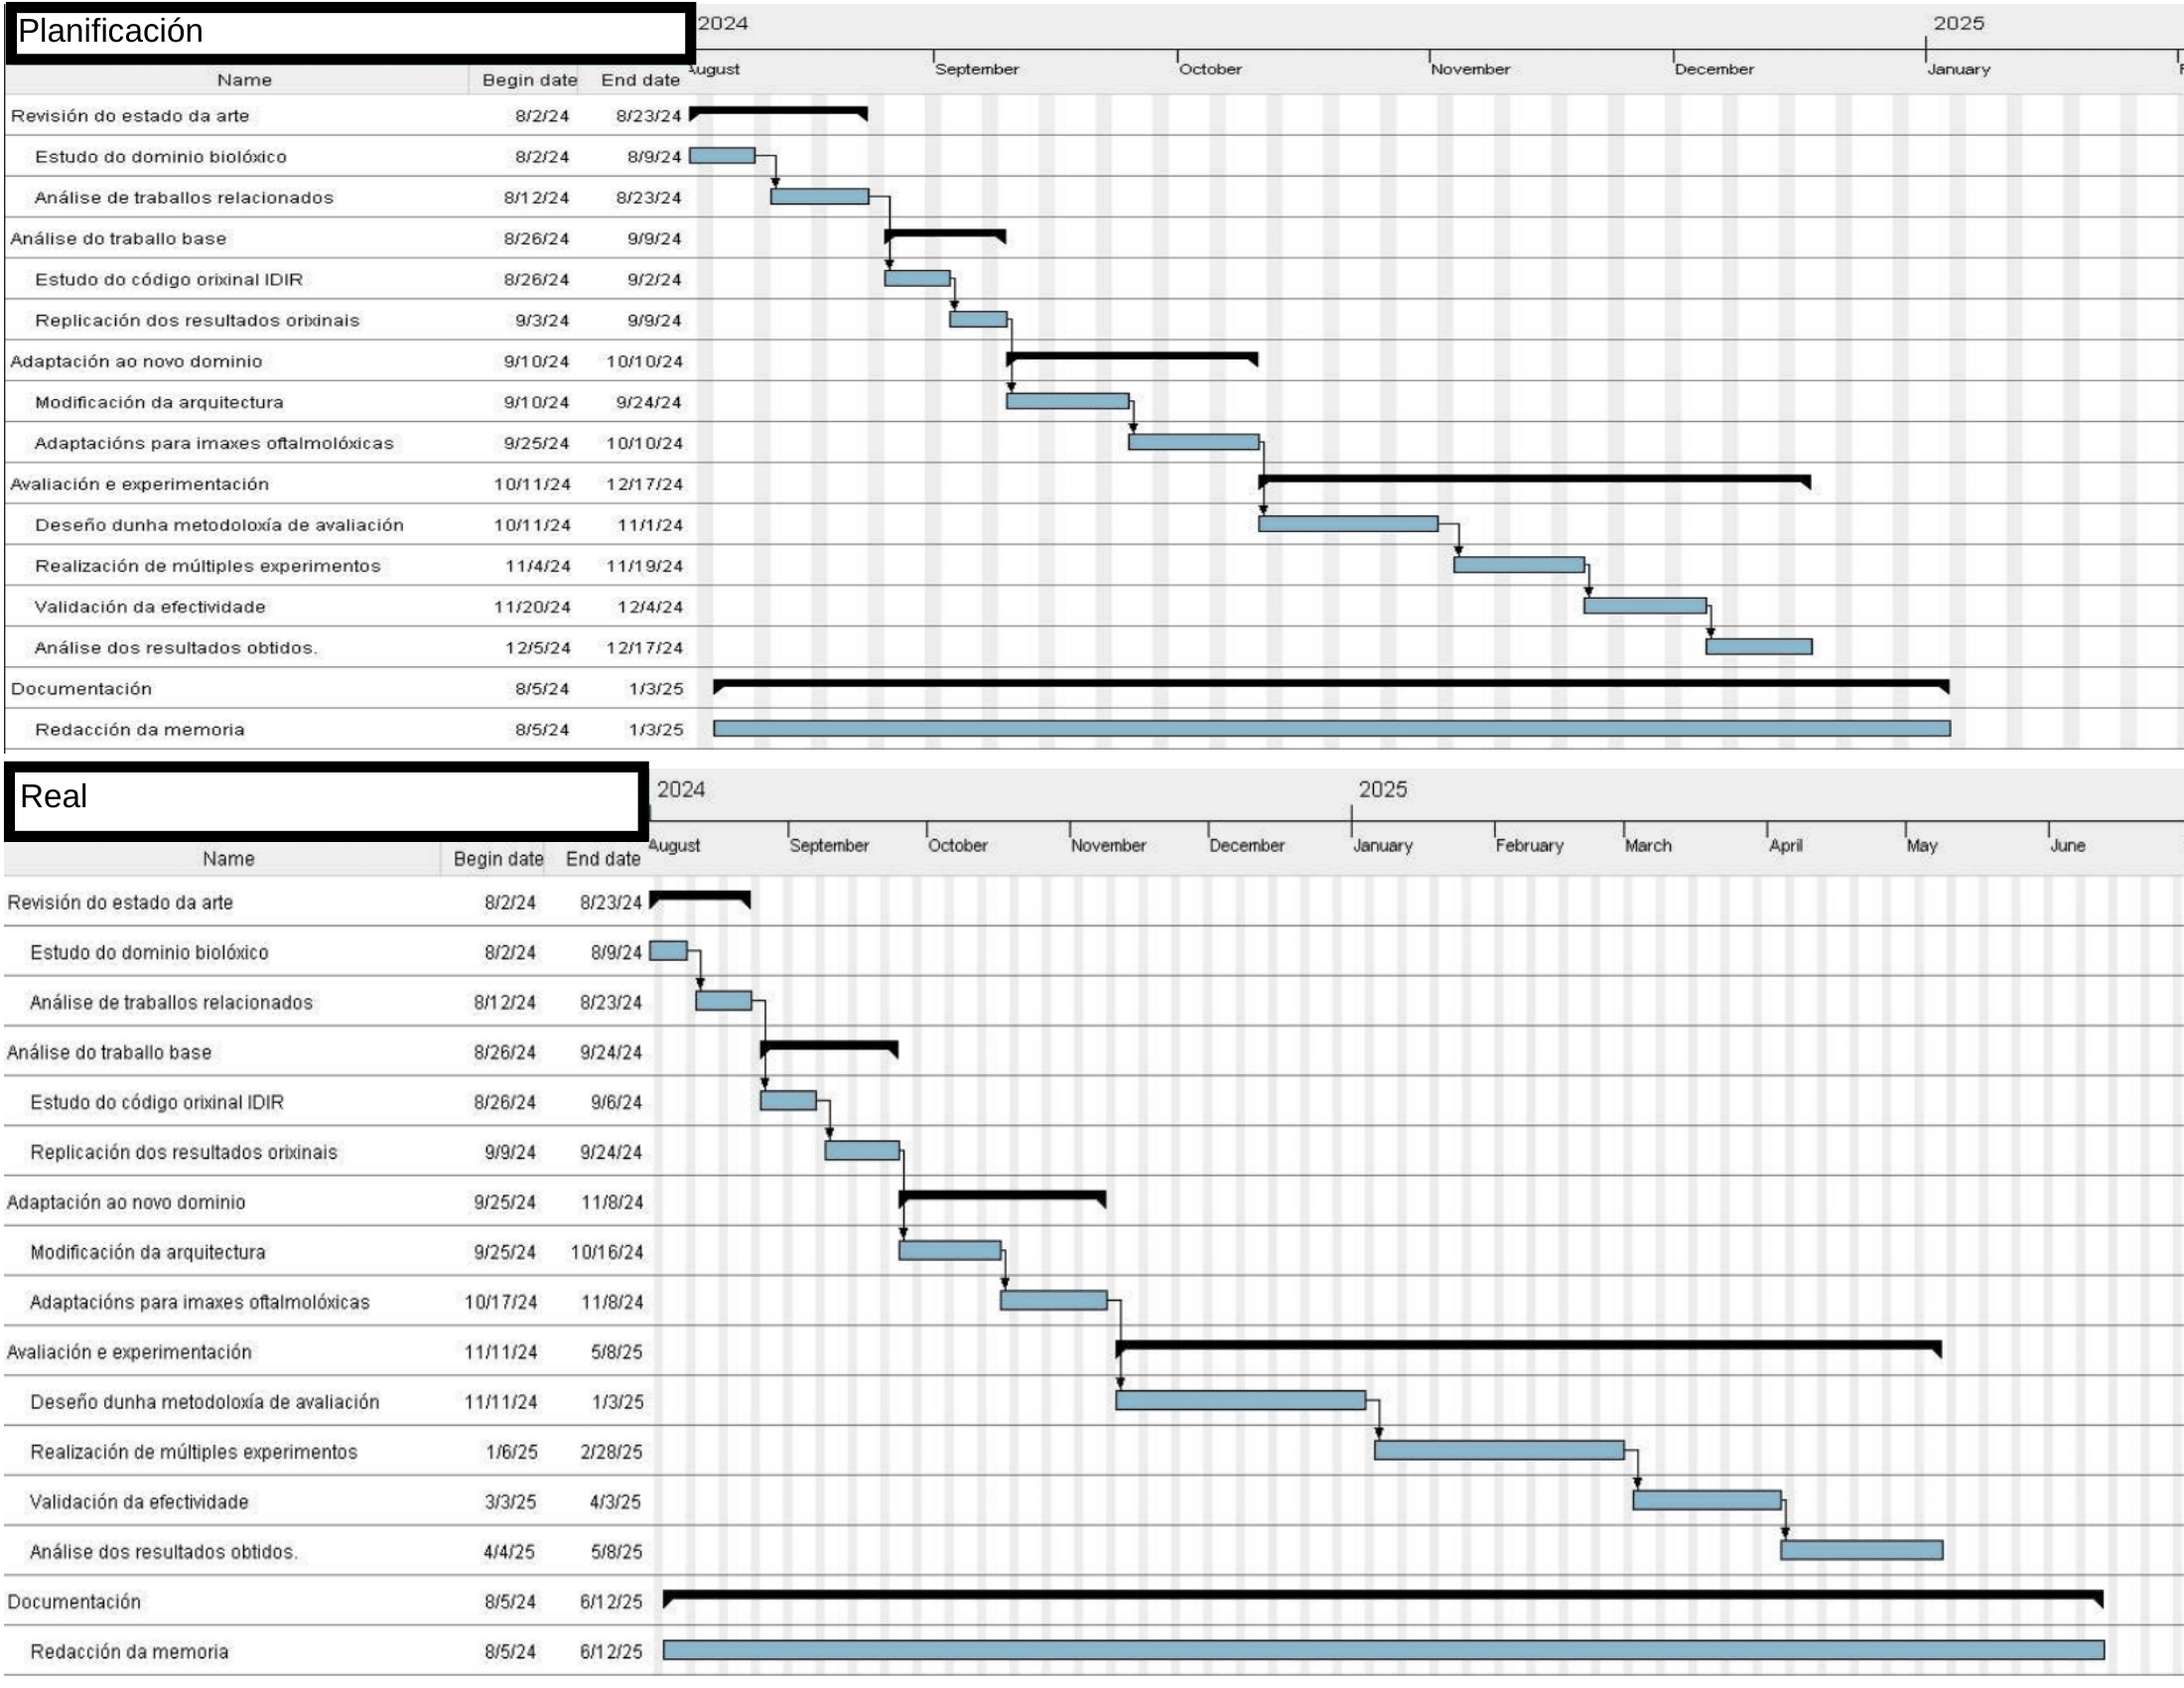
\includegraphics[height=1\textwidth, angle=90]{imaxes/gants-1.png}
    \caption{Diagramas de Gantt da planificación do proxecto e duración real de cada fase}
    \label{fig:planificacion_proxecto}
\end{figure}

\section{Recursos utilizados}
\label{sec:Recursos utilizados}

\subsection{Software}
\label{subsec:Software}

Xa que parte do traballo consiste en adaptar un traballo previo, 
decidíuse empregar moito do mesmo software ca o traballo orixinal para facilitar a implementación e reproducibilidade.
O mais relevante é PyTorch, unha librería de código aberto para Python que facilita o desenrolo de redes neuronais. Utilizáronse as versións de Python 3.12.3 e CUDA 12.2. Tamén se empregan librerías de apoio como NumPy (para traballar con matrices), Matplotlib (visualización), OpenCV ou scikit-learn (manexo de imaxes).

Outro software empregado inclúe VSCode (IDE), Git (control de versións) e LaTeX (redacción de memoria).

\subsection{Hardware}
\label{subsec:Hardware}

O proxecto foi desenrrolado nun ordenador portátil conectado por ssh a un servidor con GPU. 
Utilizáronse dous servidores diferentes, un montado por min\footnote{\url{https://blog.m19182.dev/writings/Building-my-Homelab}} e outro facilitado polo grupo de investigación VARPA (Visión Artificial y Reconocimiento de Patrones).

A gran parte dos experimentos foron realizado no primeiro, mais para poder executar o proxecto cas imaxes na súa resolución orixinal foi necesario empregar o segundo 
debido ás limitacións de memoria da GPU. Na táboa \ref{tab:comparativa_servidores} móstrase unha comparativa entre os servidores utilizados, indicando as principais características de hardware de cada un.

\begin{table}[tbp]
\centering
\begin{tabular}{|c|c|c|}
\hline
\textbf{Característica} & \textbf{Homelab} & \textbf{Servidor VARPA} \\ \hline
Procesador & AMD Ryzen 9 5950X&  AMD Ryzen Threadripper 3960X \\ \hline
GPU & NVIDIA RTX 3090 & NVIDIA RTX A6000  \\ \hline
\end{tabular}
\caption{Comparativa entre os servidores utilizados}
\label{tab:comparativa_servidores}
\end{table}


\subsection{Conxuntos de datos}
\label{subsec:Conxuntos de datos}
Para o desenrolo do proxecto empregáronse dous conxuntos de datos diferentes:

\begin{itemize}
    \item \textbf{RFMID:} 3200 imaxes de fondo de ollo en cor con resolución 1712x1712.
    \item \textbf{FIRE:} 134 pares de imaxes de retinas en cor, cun tamaño de 2912×2912 pixels
\end{itemize}

Estos son descritos en maior detalle na sección \ref{sec:Conxuntos de datos}.

\subsection{Estimación de custos}
\label{subsec:Estimación de custos}

Os custos do hardware son ignorados xa que xa estaba dispoñible antes da realización do proxecto.

Os custos dos recursos humanos calcúlanse para un estudante e dous titores, resultando nun custo estimado de 20.680€, IVE incluído. A táboa \ref{tab:estimacion_custos} mostra a estimación de custos dos recursos humanos desglosados, considerando un estudante a 20€/hora e titores a 35€/hora.

\begin{table}[h]
\centering
\begin{tabular}{|c|c|c|c|}
\hline
\textbf{Recurso} & \textbf{Custo por hora} & \textbf{Horas estimadas} & \textbf{Custo total} \\ \hline
Estudante & 20€ & 880h & 17.600€ \\ \hline
Titor 1 & 35€ & 44h & 1.540€ \\ \hline
Titor 2 & 35€ & 44h & 1.540€ \\ \hline
\end{tabular}
\caption{Estimación de custos dos recursos humanos (IVE incluído)}
\label{tab:estimacion_custos}
\end{table}

\section{Seguimento da planificación}
\label{sec:Seguimento da planificación}

A planificación do proxecto foi revisada periodicamente segundo as fases do proxecto, e para identificar desviacións respecto ao plan inicial.

Pese a que nas fases iniciais do proxecto se respectou a planificación, a fase de adaptación ao novo dominio e a fase de avaliación e experimentación sufriron retrasos significativos.

A fase de adaptación ao novo dominio requiriu máis tempo do esperado debido á complexidade das modificacións necesarias para adaptar o modelo a imaxes 2D, así como á necesidade de realizar múltiples probas para garantir o correcto funcionamento do modelo adaptado. A fase de avaliación tamén se viu afectada, xa que requiriu máis tempo do esperado para deseñar unha metodoloxía de avaliación adecuada. Finalmente, a fase de experimentación requiriu máis tempo do previsto, en parte debido aos malos resultados obtidos inicialmente, que obrigaron a revisar en profundidade o código e implementar novas probas para asegurar a correcta implementación.
En total, isto conlevou un retraso de aproximadamente 18 semanas respecto á planificación inicial.

A fase final de análise de resultados e redacción da memoria tamén se viu afectada, aínda que en menor medida, o que conlevou un retraso adicional de 2 semanas, resultando nunha duración total do proxecto de 40 semanas, fronte ás 20 semanas inicialmente previstas.

Na figura \ref{fig:planificacion_proxecto} móstrase o diagrama de Gantt actualizado, que reflicte a duración real de cada fase do proxecto.

\subsection{Estimación de custo real}
\label{subsec:Estimación de custo real}

A estimación de custo do proxecto foi de 20.680€, como se indicou na sección \ref{subsec:Estimación de custos}. Non obstante, debido aos retrasos no desenvolvemento do proxecto, o custo real aumentou de forma proporcional ao tempo extra empregado.

Dado que o proxecto se estendeu durante 20 semanas máis do previsto (o dobre da planificación inicial), o custo real estimado ascende a 41.360€ (IVE incluído).
 \chapter{Traballo Realizado}
\label{chap:Traballo Realizado}

\lettrine{N}{este} capítulo preséntase o traballo realizado para adaptar o framework IDIR ao rexistro de imaxes de retina en 2D. Comézase cunha vista xeral do proceso e unha descripción detallada do método IDIR orixinal, seguido da explicación das modificacións realizadas para adaptar o sistema ás características específicas das imaxes de fondo de ollo. Posteriormente, descríbense os conxuntos de datos empregados, o deseño experimental desenvolvido e os métodos de avaliación utilizados para validar os resultados.

\section{Vista Xeral}
\label{sec:VistaXeral}

O traballo realizado centrouse na adaptación do framework IDIR, orixinalmente deseñado para 4D-CT torácicas, ao problema específico do rexistro de imaxes de fondo de ollo en 2D. Esta tarefa requiriu modificar a arquitectura da rede neuronal para operar en dúas dimensións, reformular os termos de regularización e adaptar os procesos de adestramento e avaliación para o novo dominio.
Para optimizar o modelo, deseñouse un proceso de experimentación sistemático e desenvolvéronse metodoloxías de adestramento específicas. Entre elas destacan a creación de estratexias de mostraxe que priorizan rexións de interese anatómico e técnicas como o axuste dinámico de hiperparámetros para refinar a converxencia do modelo.

Finalmente, para validar os resultados, construíuse un marco de avaliación que foi aplicado sobre o datasets FIRE (que contén parellas de imaxes reais con diferentes graos de superposición e variacións anatómicas) e RFMiD (transformacións lineais xeneradas), o que permite xulgar distintas características da rede. A avaliación combinou métricas cuantitativas obxectivas e a análise cualitativa visual para garantir a calidade e o realismo das deformacións obtidas.

\section{IDIR}
\label{sec:IDIR}

IDIR (Implicit Deformable Image Registration) é un método de aliñamento de imaxes baseado en redes neuronais. 
A súa principal diferenza frente a unha rede convolucional tradicional é que, 

O que se propón é optimizar directamente o DFV facendo uso dunha representación implícita, de forma que a deformación está representada nos propios pesos dun MLP \cite{wolterink2021implicit}.

Outros traballos como NIR \cite{sun2024medicalimageregistrationneural} ou NODEO \cite{nodeo} propoñen métodos de rexistro similares que tamén fan uso de representacións implícitas das deformacións, aplicados a resonancias magnéticas do cerebro.
%  baseados en Neural ODE (ODE-Nets)\cite{neuralode}, unha familia de modelos de aprendizaxe profundo que trata a rede como un sistema continuo en lugar de unha secuencia de capas discretas.

\subsection{Arquitectura}
\label{subsubsec:Arquitectura}

Faise uso dun MLP de 3 capas, e determinaron experimentalmente que obtiñan mellor resultado con 256 unidades por capa que 128.
Por cada epoch de entrenamento (2500 en total), 10000 puntos son muestreados aleatoriamente do espazo de coordenadas dentro da máscara.
O término de perda é a 'normalized cross-correlation' entre os valores dos píxeles muestreados na imaxe fixa e os correspondentes da imaxe móbil.
Utilizan Adam de optimizador, cun learning rate de 0.0001.

\subsubsection{Función de activación}
\label{subsubsec:Función de activación}

Unha elección estándar para a función de activación é \textbf{ReLU}:

\[
f(x) = \max(0, x) = \begin{cases} 
x & \text{si } x > 0 \\ 
0 & \text{si } x \leq 0 
\end{cases}
\]

Non obstante, para redes de representación implícita como ca que estamos traballando, esta ten unha serie de desventaxas.

As ReLUs teñen un sesgo cara a sinais de baixa frecuencia \cite{rahaman2019spectralbiasneuralnetworks}, 
 o que significa que o modelo pode ter dificultades para representar pequenas deformacións locais no rexistro de imaxes.
 
\cite{ziyin2020neuralnetworksfaillearn} demostraron que a gran parte das funcións de activación utilizadas en redes neuronais (ReLU, tanh, sigmoide e todas as súas variantes)
son incapaces de extrapolar función periódicas sinxelas debido á súa tendencia a converxer cara a comportamentos lineais cando se extrapolan fóra do rango de adestramento. 

Existen varias formas de superar este sesgo, como preprocesar as coordenadas de entrada con funcións de activación periódicas \cite{mildenhall2020nerfrepresentingscenesneural} 
ou substituír a función de activación ReLU por unha función de activación periódica \cite{sitzmann2020implicitneuralrepresentationsperiodic}.

Neste traballo escollemos a segunda opción, utilizando unha función de activación periódica de tipo \textbf{SIREN}:

\[
f(x) = \sin(ax + b), \quad \text{con} \quad a, b \in \mathbb{R}
\]

Unha vantaxe engadida das funcións de activación periódicas nas redes SIREN é que poden ser diferenciadas varias veces, 
o que expande substancialmente o conxunto de termos de regularización que se poden empregar na rede, como veremos na seguinte sección.

larger frequencies appear in the networks for weights with larger magnitudes.

Outros traballos como \cite{mildenhall2020nerfrepresentingscenesneural} non utiliza unha función de activación periódica, mais para a representación adecuada de zonas de alta frecuencia 
utilizaron codificación posicional, que xa as incorpora de forma implícita na rede con bós resultados. 

Outra das vantaxes que ten SIREN é que é unha función suave ou infinitamente diferenciable, é dicir, que admite derivadas de calquer orde.
Outros exemplos de funcións de activación infinitamente diferenciables son:

Sigmoide:  
\[
f(x) = \frac{1}{1 + e^{-x}}
\]
Tangente Hiperbólica:  
\[
f(x) = \tanh(x) = \frac{e^x - e^{-x}}{e^x + e^{-x}}
\]

Softplus:  
\[
f(x) = \ln(1 + e^x)
\]


\paragraph{Inicialización de pesos}

En \cite{sitzmann2020implicitneuralrepresentationsperiodic} propuxeron unha inicialización específica para as redes SIREN, 
a cal consiste en inicializar a primeira capa de xeito que a función seno recorra múltiples períodos sobre o intervalo [−1,1][−1,1].
Isto conséguese multiplicando os pesos da primeira capa por un factor de escala ω0, sobre o cal recomendan ω0=30.
A fórmula para a inicialización dos pesos da primeira capa é a seguinte:

\begin{figure}[tbp]
    \centering
    \[
    w_i \sim U\left[ -\frac{1}{n}, \frac{1}{n} \right]
    \]

\caption{Inicialización primera capa}
\end{figure}

onde n é o número de neuronas de entrada (o tamaño da capa anterior).

As seguintes capas inicialízanse da seguinte forma:
\begin{figure}[tbp]
    \centering
    \[
    w_i \sim U\left[ -\frac{\sqrt{\frac{6}{n}}}{w}, \frac{\sqrt{\frac{6}{n}}}{w} \right]
    \]
    \caption{Inicialización seguintes capas}
\end{figure}

Desta forma asegurase que a entrada a cada activación sinusoidal está distribuída normalmente cunha desviación estándar de 1,
 o que debería mellorar a estabilidade e converxencia durante o adestramento da rede.
Unha consecuencia desto é que, xa que os propios pesos da rede representan a deformación, inicialmente a rede comeza cunha deformacion moi similar en todos os casos, que o entrenamento deberá corrixir.

En \cite{sireninit} implementan unha versión simplificada de SIREN para facilitar o estudo destas, 
e propoñen melloras proceso de inicialización. Unha delas e utilizar a distribución Kaiming (He) en lugar da uniforme.
Tamén propoñen un método para escoller un valor de w apropiado según o problema a resolver.

\subsubsection{Termos de loss}
\label{subsubsec:Termos de loss}

O termo de perda é a función que se optimiza durante o adestramento, e é o que guía a rede cara a unha solución óptima.
Esta cuantifica a discrepancia entre a saída da rede e o resultado desexado.

Para a tarefa de rexistro de imaxes, utilízanse dúas categorías principais de métricas para avaliar o aliñamento entre imaxes: 
as métricas baseadas no erro e as métricas baseadas na similitude. As métricas baseadas no erro (MSE, L1...) miden as diferenzas píxel a píxel entre as imaxes, 
sendo máis sensibles a diferenzas locais e proporcionando unha medida absoluta. 
As métricas baseadas na similitude (NCC, SSIM...) teñen en conta patróns estructurais e relacións estatísticas entre as imaxes, sendo máis robustas fronte a variacións na iluminación e pequenos desprazamentos.
\cite{simmetric}

Os principais termos de perda valorados para este traballo son:

\begin{itemize}
    % Error-based metrics
    \item \textbf{MSE (Mean Squared Error)}:
    Erro cadrático promedio entre á imaxe fixa e a móbil. É sensible a valores atípicos e ruido.
    \[
    \text{MSE} = \mathbb{E}[(Y - \hat{Y})^2] = \frac{1}{N} \sum_{i=1}^{N} (y_i - \hat{y}_i)^2
    \]
    onde \( y_i \) é o valor do pixel da imaxe fixa, \( \hat{y}_i \) é o valor do pixel da imaxe móbil, e \( N \) é o número total de píxeles. \cite{Palubinskas02012017}

    Regulizador Hiperelástico en 2D   \item \textbf{L1 (Mean Absolute Error)}:
    Mide o error absoluto promedio. Menos sensible a valores atípicos que MSE.
    \[
    \text{L1} = \mathbb{E}[|Y - \hat{Y}|] = \frac{1}{N} \sum_{i=1}^{N} |y_i - \hat{y}_i|
    \]

    % Robust error metrics
    \item \textbf{Huber Loss}:
    Combina MSE e L1, sendo cadrática para errores pequenos e lineal para errores grandes.
    \[
    \text{Huber}(y, \hat{y}) = \begin{cases}
    \frac{1}{2}(y - \hat{y})^2 & \text{se } |y - \hat{y}| \leq \delta \\
    \delta(|y - \hat{y}| - \frac{1}{2}\delta) & \text{noutro caso}
    \end{cases}
    \]
    onde \( \delta \) é un hiperparámetro que define o punto de transición entre os comportamentos cadrático e lineal.

    \item \textbf{Smooth L1 Loss}:
    Similar a Huber Loss, pero cunha transición suave entre as rexións cadrática e lineal.
    \[
    \text{SmoothL1}(y, \hat{y}) = \begin{cases}
    \frac{1}{2}(y - \hat{y})^2 & \text{se } |y - \hat{y}| \leq 1 \\
    |y - \hat{y}| - \frac{1}{2} & \text{noutro caso}
    \end{cases}
    \]

    % Similarity-based metrics
    \item \textbf{NCC (Normalized Cross-Correlation)}:
    Evalúa a similitude entre as dúas imaxes normalizando as súas intensidades. É invariante a cambios na iluminación.
    \[
    \text{NCC} = \frac{\sum_{i=1}^{N} (y_i - \mu_y)(\hat{y}_i - \mu_{\hat{y}})}{\sqrt{\sum_{i=1}^{N} (y_i - \mu_y)^2 \sum_{i=1}^{N} (\hat{y}_i - \mu_{\hat{y}})^2}}
    \]
    onde \( \mu_y \) e \( \mu_{\hat{y}} \) son as medias das imaxes fixa e móbil, respectivamente.

    \item \textbf{SSIM (Structural Similarity Index)}:
    Evalúa a similitude estructural entre as dúas imaxes, considerando luminancia, contraste e estructura.
    \[
    \text{SSIM}(y, \hat{y}) = \frac{(2\mu_y\mu_{\hat{y}} + C_1)(2\sigma_{y\hat{y}} + C_2)}{(\mu_y^2 + \mu_{\hat{y}}^2 + C_1)(\sigma_y^2 + \sigma_{\hat{y}}^2 + C_2)}
    \]
    onde \( \mu_y \), \( \mu_{\hat{y}} \) son as medias, \( \sigma_y \), \( \sigma_{\hat{y}} \) son as desviacións estándar, \( \sigma_{y\hat{y}} \) é a covarianza, e \( C_1 \), \( C_2 \) son constantes para evitar divisións entre cero. \cite{Palubinskas02012017}
\end{itemize}

Debido á natureza das imaxes de retina, onde poden existir diferencias de iluminación e contraste entre as imaxes fixa e móbil, 
parece mais apropiado empregar métricas baseadas na similitude como NCC ou SSIM.

NCC utilizouse a implementación de  https://github.com/BDdeVos/TorchIR/blob/main/torchir/metrics.py.

\subsubsection{Termos de regularización}
\label{subsubsec:Termos de regularización}

Debido a que o rexistro de imáxenes deformables é un problema mal planteado (ill-posed problem**), 
é común utilizar algún tipo de regularización sobre o DVF para evitar deformacións pouco realistas.
 Os métodos de rexistro baseados en redes neuronaies convolucionais (CNN) representan os DVFs
 como mostras en una cuadrícula de vóxeles, e polo tanto, solo se poden aproximar gradientes espaciais
 mediante esquemas de diferencias finitas (aproximar derivadas mediante cálculo numérico de diferencias entre valores adyacentes en la cuadrícula).
 Este é un proceso computacionalmente moi costoso e ineficiente, ademais implica errores de discretización e perdas de precisión.


Facendo uso de representacións implícitas, todas as operación son diferenciables, e os gradientes poden
 ser computados facilemente de forma analítica en lugar de ter que aproximalos, facendo uso da librearía de autodiferenciación de PyTorch.

Utilizando ReLU como función de activación, a rede é diferenciable unha vez, mentres que utilizando
 unha función de activación periódica (como SIREN), a rede é diferenciable todas as veces que se precise.
Desta forma, podemos calcular calquera número de termos de regularización e incluilos na optimización da rede.

Algúns exemplos de termos de regularización que se poden empregar son:
\begin{itemize}
    \item Jacobian regularizer: 
    O determinante Jacobiano da transformación (det ∇Φ) nunha localización x é un indicador de estiramento ou compresión local.
    Un determinante Jacobiano negativo ou moi cercano a 0 indica que están a ocurrir dobreces e a transformación non será invertible.
    A matriz jacobiana é a matriz que contén todas as derivadas parciais da función de transformación (calculado mediante gradientes).
    O termo de regularización do Jacobiano penaliza os valores do determinante Jacobiano que se desvían de 1, 
    tentando preservar áreas locais e evitar estiramentos ou dobreces extremas.


    \begin{figure}[tbp]
        \centering
        \[
        S^{jac}[\Phi] = \int_{\Omega} \left| 1 - \det \left( \nabla \Phi \right) \right| \, dx
        \]
        \caption{Regulizador Jacobiano}
    \end{figure}

    Ω representa o dominio ou rexión do espazo sobre o cal está definida a transformación Φ.
    
    \item Hyperelastic regularizer
    Tamén se póden engadir restricións ao DVF con este termo proposto por \cite{HyperelasticRegularization}.
    Consiste en tres termos, un termo de lonxitude, un termo de área e un termo de volumen co obxetivo de controlar variacións nestes aspectos.
    O termo de lonxitude penaliza a variación da lonxitude dos vectores do DVF, sendo u a medida desplazamiento dun punto no espacio.
    A matriz de cofactores da matriz do Jacobiano da transformación controla o área, 
    A función de máximo asegura que só as expansións que sobrepasen certo límite sexan penalizadas
    O determinante da matriz do Jacobiana controla o volume, 
    e ambas penalizan o crecemento e a contracción por igual.
    αl, αa e αν son hiperparámetros que controlan a importancia de cada término.

    \begin{figure}[tbp]
        \centering
        \[
        S^{hyper}[\Phi] = \int_{\Omega} \left[ \frac{1}{2} \alpha_1 |\nabla u|^2 + \alpha_a \varphi_c (\text{cof} \nabla \Phi) + \alpha_\nu \psi(\det \nabla \Phi) \right] dx,
        \]
        \[
        \text{Funcións convexas:} \quad \varphi_c(C) = \sum_{i=1}^3 \max \left\{ \sum_{j=1}^3 C_{ji}^2 - 1, 0 \right\}^2 \quad \text{and} \quad \psi(v) = \frac{(v-1)^4}{v^2}.
        \]
        \caption{Regulizador Hiperelástico.}
    \end{figure}


    \item Bending energy penalty
    Pódese impoñer a suavidade da deformación empregando esta penalización proposta en \cite{bendingenergy}, que 
    require que as segundas derivadas do DVF sexan pequenas en todo o dominio, o que evita deformacións bruscas e discontinuas.
    Este termo non pode ser utilizado nunha rede que utilice ReLU como función de activación, xa que a segunda derivada de unha ReLU é sempre igual a 0.

    \begin{figure}[tbp]
        \centering
        \[
        S^{bending}[\Phi] = \frac{1}{8} \int_{-1}^{1} \int_{-1}^{1} \int_{-1}^{1} \left[ \left( \frac{\partial^2 \Phi}{\partial x^2} \right)^2 + \left( \frac{\partial^2 \Phi}{\partial y^2} \right)^2 + \left( \frac{\partial^2 \Phi}{\partial z^2} \right)^2 \right.
        \]
        \[
        \left. + 2 \left( \frac{\partial^2 \Phi}{\partial x \partial y} \right)^2 + 2 \left( \frac{\partial^2 \Phi}{\partial x \partial z} \right)^2 + 2 \left( \frac{\partial^2 \Phi}{\partial y \partial z} \right)^2 \right] dx\,dy\,dz
        \]
        \caption{Regulizador Bending Energy}
    \end{figure}
    
\end{itemize}

Para a implementación neste traballo modificaronse todos estos termos para que funcionaran con transfomacións de dúas dimensións en lugar de tres,
 sustituíndo o gradiente de 3 dimensión no Jacobiano por un de dúas, eliminando as derivadas parciais en z en bending energy e o termo de volume no termo hiperelástico.

\begin{itemize}
    \item Jacobian regularizer:\\
    \[
    S^{jac}[\Phi] = \int_{\Omega} \left| 1 - \det \left( \nabla \Phi \right) \right| \, dx \, dy
    \]
    \item Hyperelastic regularizer:\\
    \[
    S^{hyper}[\Phi] = \int_{\Omega} \left[ \frac{1}{2} \alpha_1 |\nabla u|^2 + \alpha_a \varphi_c (\text{cof} \nabla \Phi) \right] dx \, dy,
    \]
    \[
    \varphi_c(C) = \sum_{i=1}^2 \max \left\{ \sum_{j=1}^2 C_{ji}^2 - 1, 0 \right\}^2
    \]
    \item Bending energy penalty:\\
    \[
    S^{bending}[\Phi] = \frac{1}{8} \int_{-1}^{1} \int_{-1}^{1} \left[ \left( \frac{\partial^2 \Phi}{\partial x^2} \right)^2 + \left( \frac{\partial^2 \Phi}{\partial y^2} \right)^2 + 2 \left( \frac{\partial^2 \Phi}{\partial x \partial y} \right)^2 \right] dx \, dy
    \]
\end{itemize}

A regularización tamén ten un impacto significativo no tempo de computación, xa que require múltiples pasadas de retropropagación por época para calcular os distintos termos de penalización.
Sen regularización só se fai 1 pasada para calcular o gradiente do termo de similitude da imaxe.
Ca regularización do Jacobiano, ademais do termo de similitude, calcúlanse dúas derivadas (unha por dimensión) para obter o Jacobiano, resultando en 3 pasadas por época.
Engadindo a regularización hiperelástica (sen termo de volume), é necesario calcular unha derivada adicional para o cofactor da matriz Jacobiana, facendo un total de 4 pasadas por época.
Finalmente, ca penalización de enerxía de flexión, necesitanse derivadas segundas, o que implica 7 pasadas por época en total.
No traballo orixinal de IDIR, chegaban a usar 13 pasadas debido a que traballan en 3D.

Se os termos de regularización teñen demasiada influencia sobre o termo de loss, a rede fará transformacións moi pequenas para evitar ser penalizada, o que resultará nunha transformación insuficiente.
Por outro lado, se os termos son demasiado pequenos, a rede fará transformacións moi grandes, o que resulta nunha transformación irrealista e sobreaxustada. Isto é especialmente evidente no caso da función de activación SIREN, que tende a sobreaxustarse facilmente debido ao seu sesgo cara sinais de alta frecuencia.
A cantidade óptima de regularización depende da parexa concreta de imaxes a alinear, polo que intentaremos determinar cal é a mellor para unha mostra de imaxes.

Ademais, pese a que os diferentes termos de regularización valoran diferentes aspectos, cabe ter en conta que tamén superposición nalgunhas das propiedades que valoran.
Por exemplo, o regularizador hiperelástico pode considerarse un termo mais xeral que inclúe indirectamente penalizaciones do Jacobiano (ambos penalizan as "dobreces") e de suavidade das transfomacións (como fai o bending pero en menor grado).

\subsubsection{Learning rate e batch size}
\label{subsubsec:Learning rate e batch size}

O learning rate é un parámetro do optimizador (Adam neste caso) que regula o tamaño dos axustes efectuados aos parámetros do modelo durante cada iteración de actualización. 
Determina a magnitude do cambio aplicado para minimizar a función de perda, afectando tanto a velocidade de converxencia como a estabilidade do proceso de aprendizaxe.
Un learning rate demasiado alto pode provocar que a rede diverxa, mentres que un learning rate demasiado baixo pode resultar en converxencia lenta ou quedar atrapado en mínimos locais.

Debido á natureza da rede, o batch size utilzado ten unha relación directa co learning rate, polo que tentaremos determinar a relación óptima entre ambos.

Unha das heurísiticas mais comúns para relacionar o learning rate e o batch size é a regla de escalado linear \cite{goyal2018accuratelargeminibatchsgd}. 
A regla indica que o learning rate óptimo debe escalarse linearmente co tamaño do batch size. 

Unha forma de explicar isto é, xa que con batches mais grandes temos unha mellor aproximación do gradiente real, é posible utilizar un learning rate maior sen que a rede diverxa. \cite{kexuefm}

O batch size nesta rede representa o número de coordenadas amostradas aleatoriamente do espazo de coordenadas dentro da máscara.

\subsection{Método}
\label{subsubsec:Método}

Sendo o obxetivo encontrar unha transformación espacial óptima entre a imaxe móbil e a imaxe fixa,
é necesario obter a función de deformación  Φ(x) = u(x) + x que mapea cada coordenada x na imaxe móbil a unha coordenada na imaxe fixa, 
de forma que a coordenada x na imaxe fixa corresponda anatomicamente á coordenada Φ(x) na imaxe móbil.
Este problema pode ser formulado como un problema de optimización onde $L_{data}$ é unha métrica de similitude entre as imaxes fixa ($F$) e móbil ($M$), $L_{reg}$ é un termo de regularización na transformación Φ, e α é un termo de ponderación.
\begin{equation}
    \hat{\Phi} = \operatorname*{Arg\,min}_{\Phi} L_{data}(M \circ \Phi, F) + \alpha L_{reg}(\Phi)
\end{equation}


A principal innovación que introduce IDIR\cite{wolterink2021implicit} é que a transformación Φ está implícitamente representada na rede neuronal.

Comparado cunha CNN tradicional, esta rede non recibe valores de intensidade de píxel como entrada,
senón que recibe coordenadas espaciais (continuas) e devolve unha nova coordenada.
Xa que os pesos da rede definen a transformación, estos poden ser optimizados directamente 
facendo uso dunha métrica de similitude como función de perda.

Parametrizar a función de deformación como unha \glossary{INR} dentro dun \glossary{MLP} ten varias vantaxes para o rexistro de imaxes.
En primeiro lugar, a representación da transformación é continua e polo tanto independente da resolución da imaxe, 
grazas a iso o mesmo modelo poder ser empregado para imaxes de calquer tamaño, ao contrario dunha CNN tradicional 
que ten que ser adaptada para cada resolución.

Segundo, facelo desta forma permite aproveitar as capacidades de librerías como PyTorch para calcular os gradientes da transformación respecto das coordenadas.
Isto permite obter gradientes máis precisos que as aproximacións por diferencias finitas 
e permite aproveitar unha gran cantidade de literatura sobre regularización eficientes en imaxes médicas.

Terceiro, pódese modificar a función de activación empregada na rede para axustala ás necesidades particulares da tarefa de rexistro de imaxes.

O \gls{NTK} describe cómo un modelo de red neuronal responde a cambios en sus parámetros durante el entrenamiento,
e dependendo da función de activación empregada, o NTK varía e a rede pode ser máis ou menos sensible a certas deformacións.

Finalmente, entrenaráse unha nova rede por cada parella de imaxes, sendo esta unha rede bastante pequena en comparación e prescindindo da necesidade de grandes conxuntos de datos para o seu adestramento.

\subsection{Replicación de resultados}
\label{subsec:Replicación de resultados}

Replicáronse os resultados obtidos por Wolterink et al. \cite{wolterink2021implicit} que se mostran na táboa \ref{tab:comparison}.

\begin{table}[ht]
    \centering
    \caption{Replicación dos resultados de IDIR}
    \begin{tabular}{c|c}
        Scan & {IDIR / Replicación} \\
        1  & 0.76 (0.94) / 0.79 (0.92) \\
        2  & 0.76 (0.94) / 0.71 (0.89) \\
        3  & 0.94 (1.02) / 0.95 (1.01) \\
        4  & 1.32 (1.27) / 1.32 (1.22) \\
        5  & 1.23 (1.47) / 1.23 (1.46) \\
        6  & 1.09 (1.03) / 1.15 (1.04) \\
        7  & 1.12 (1.00) / 1.11 (0.99) \\
        8  & 1.21 (1.29) / 1.20 (1.28) \\
        9  & 1.22 (0.95) / 1.16 (0.99) \\
        10 & 1.01 (1.05) / 1.09 (1.05) \\
        Promedio & 1.07 / 1.07 (1.08) \\
    \end{tabular}
    \label{tab:comparison}
\end{table}

\section{Adaptación a 2D}
\label{sec:Adaptación a 2D}

Para adaptar o modelo IDIR a 2D, é necesario modificar a arquitectura da rede para que funcione con imaxes bidimensionais.
A arquitectura orixinal de IDIR ten unha entrada de 3 dimensións (x, y, z) e unha saída de 3 dimensións (dx, dy, dz),
mentres que a nosa rede ten unha entrada de 2 dimensións (x, y) e unha saída de 2 dimensións (dx, dy).

Modificáronse as capas de entrada e saída da rede para que acepten coordenadas bidimensionais (orixinalmente [3, 256, 256, 256, 3], agora [2, 256, 256, 256, 2]).

Foi necesario modificar as funcións de interpolación, que antes interpolaban valores tridimensionais e agora interpolan valores bidimensionais.

Tamén adaptáronse os termos de regularización para que funcionen con coordenadas bidimensionais, como se detalla na sección \ref{subsubsec:Termos de regularización}.

Finalmente, o proceso de avaliación tivo que implementarse dende 0 para adaptarse ao novo formato de imaxes e ground truth.

\subsection{Proceso de Rexistro}
\label{subsec:Proceso de Rexistro}

O rexistro de cada par de imaxes (fixa e móbil) trátase como un problema de optimización independente. Para cada par, adéstrase unha nova rede neuronal dende cero cuxo único obxectivo é aprender a deformación específica que aliña esas dúas imaxes.

Primeiramente, crease unha instancia do MLP coa arquitectura 2D e defínense os hiperparámetros como a función de activación, a métrica de perda e termos de regularización que se aplicarán. A inicialización dos pesos da rede é un paso de especial relevancia. 

Unha vez inicializada a rede, xérase un tensor de coordenadas que contén a localización (x, y) de todos os píxeles que se atopan dentro da máscara da imaxe fixa. Este tensor representa o espazo de coordenadas completo sobre o que a rede aprenderá a deformación.

A continuación, comeza o bucle de adestramento, que se repite durante un número predefinido de épocas (epochs). En cada iteración dentro dunha época, realízase o seguinte proceso:
\begin{itemize}
    \item \textbf{Mostraxe de Coordenadas:} En lugar de procesar a imaxe enteira en cada paso, selecciónase un subconxunto de puntos do tensor de coordenadas igual ao tamaño de batch. A estratexia de mostraxe é un compoñente crítico que foi obxecto de experimentación neste traballo.

    \item \textbf{Predición e Aplicación da Transformación:} As coordenadas (x, y) mostreadas introdúcense na rede. O MLP actúa como unha función de deformación implícita, devolvendo para cada coordenada de entrada un vector de desprazamento (dx, dy). 

    \item \textbf{Cálculo da Perda (Loss):} Para cuantificar o ben que a deformación aliña as imaxes, compáranse os valores de intensidade nos nos puntos seleccionados. Para cada coordenada orixinal $(x,y)$ na imaxe fixa, obtense o valor de intensidade correspondente na imaxe móbil na coordenada transformada $(x + dx, y + dy)$. Como esta última adoita ser unha posición non enteira, utilízase interpolación para estimar o seu valor de intensidade. A métrica de perda (NCC, SSIM, etc.) calcula a discrepancia entre o conxunto de intensidades da imaxe fixa e o das intensidades obtidas da imaxe móbil transformada.

    \item \textbf{Retropropagación e Actualización:} Ao valor da perda de similitude súmanselle os termos de penalización calculados a partir dos regularizadores. O valor de perda total resultante utilízase para calcular os gradientes respecto aos pesos da rede mediante retropropagación. Finalmente, o optimizador (Adam) utiliza estes gradientes para actualizar os pesos do MLP, axustándoos lixeiramente na dirección que minimiza a perda.
\end{itemize}

Este ciclo repítese ata completar todas as épocas. Ao final do adestramento, os pesos optimizados da rede encapsulan a función de deformación continua e específica para ese par de imaxes.

É crucial subliñar que a tarefa de rexistro de retinografías difire substancialmente da de pulmóns. Por este motivo, non é posible asumir que os hiperparámetros óptimos do traballo orixinal sexan válidos para este novo dominio, o que xustifica a extensa experimentación realizada.

\section{Conxuntos de datos}
\label{sec:Conxuntos de datos}

\subsection{FIRE}
\label{subsec:FIRE}

 Está composto por 134 pares de imaxes de retinas, con un tamaño de 2912 × 2912 pixels e un \gls{FOV} de 45◦× 45◦.
 Están clasificadas en 3 categorías según o grado de superposición e a presenza de diferencias anatómicas: \textit{S}, \textit{P} e \textit{A}. \cite{FIRE}

 \begin{figure}[tbp]
    \centering
    \setlength{\tabcolsep}{8pt} % Adjust column spacing
    \begin{tabular}{|c|c|c|c|}
        \hline
        \textbf{Categoría} & \textbf{Nº de pares de imaxes} & \textbf{Superposición (\%)} & \textbf{Diferenzas Visuais} \\
        \hline
        \textbf{\textit{\textsf{S}}} & 71 & > 75 & Non \\
        \hline
        \textbf{\textit{\textsf{P}}} & 49 & < 75 & Non \\
        \hline
        \textbf{\textit{\textsf{A}}} & 14 & > 75 & Si \\
        \hline
    \end{tabular}
    \caption{Clasificación dos pares de imaxes en categorías.}
    \label{tab:categorias}
\end{figure}
\FloatBarrier

Inclúe 10 puntos de referencia para cada imaxe, que se utilizan para a avaliación do rexistro, así como unha máscara por cada imaxe que indica a localización dos píxeles con información de cor.

\begin{figure}[tbp]
    \centering
    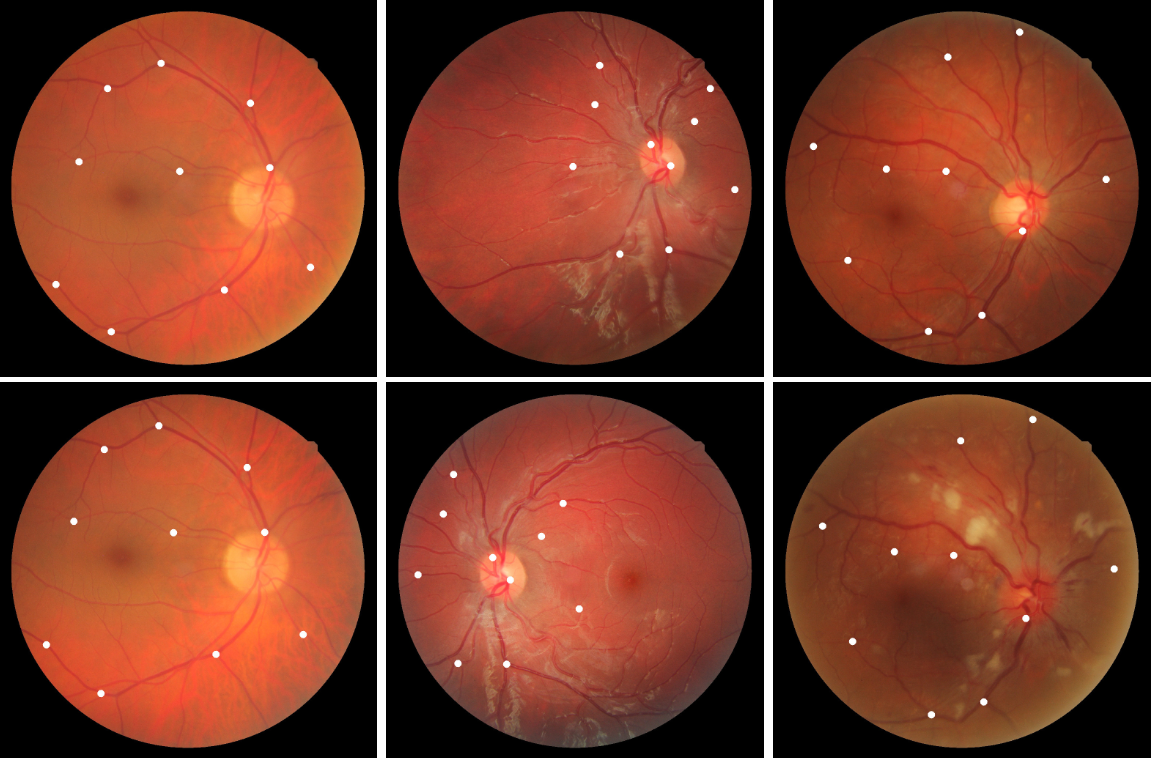
\includegraphics[width=0.8\textwidth]{imaxes/fire-ej.png}
    \caption{Exemplo de imaxes do conxunto de datos FIRE \cite{FIRE} cos puntos de control indicados. De esquerda a dereita, categorías \textit{\textsf{S}}, \textit{\textsf{P}}, \textit{\textsf{A}} .}
    \label{fig:fire_ej}
\end{figure}

\subsection{RFMID}
\label{subsec:RFMID}

O conxunto de datos RFMiD \cite{RFMiD} proporciona 3200 imaxes de fondo de ollo en cor con resolución 1712x1712, etiquetadas según se teñen algunha anomalía ou non. 
Tamén proporciona etiquetas para 45 diferentes anomalías anotadas por expertos.

Para utilizalo neste traballo, seleccionamos unha submostra e xeramos transformacións aleatorias. Gardamos as imaxes orixinais e as transformadas así como as matrices de transformación asociadas para a posterior avaliación.
Tamén se divide entre transfomacións de cor e de xeometría.

% \dots preguntar David

\subsection{Diferencias entre os datasets}
\label{subsec:Diferencias entre os datasets}

Unha vantaxe de utilizar dous conxutos de datos diferentes é que cada un deles ten características únicas que permiten avaliar o modelo en diferentes contextos.
A principal diferencia é que RMiFD é un conxunto de datos sintético, no cal non introducimos diferenzas de cor e sempre teñen unha superposición do 100\%, polo que o único que se avalia é a capacidade do modelo para realizar os rexistros xeométricos.
Polo contrario, FIRE é un conxunto de datos real, no cal existen cambios na iluminación, contraste, superposición e demais diferencias visuais, polo que se avalía a capacidade do modelo para realizar rexistros en condicións moito máis adversas.

\section{Diseño de Experimentos}
\label{sec:Diseño de Experimentos}

O deseño de experimentos é un proceso sistemático que busca determinar a influencia de diferentes factores sobre un resultado específico. Neste caso, o obxetivo é avaliar como diferentes parámetros afectan á calidade do rexistro de imaxes.

O custo computacional é un factor moi importante a ter en conta, xa que cada combinación de parámetros require un adestramento completo da rede por cada parella de imaxes, o que implica un alto custo enerxético e de tempo.
Por exemplo, para probar unha combinación de parámetros sobre FIRE haberá que entrenar unha rede por cada parella de imaxes das 134 do conxunto de datos. 
A un tempo de adestramento de 3 minutos por parella, o adestramento completo levaría mais de 6 horas por cada combinación de parámetros, cunha pegada de memoria de arredor de 5 GB de VRAM.
O custo temporal e de memoria dependen de varios factores, sendo os mais relevantes a regularización empregada, a resolución da imaxe, o tamaño do batch size e a función de activación.
En concreto, SIREN ten un custo computacional moito maior que ReLU, requerindo arredor do doble de tempo e memoria para adestrar a rede.

Debido ao gran número de factores a ter en conta, adoptouse un enfoque de experimentación en fases.

Inicialmente realizáronse experimentos iniciais para identificar os rangos de parámetros máis prometedores utilizando unha submostras representativa de 14 parellas de imaxes de cada categoría do dataset FIRE, co obxectivo: Reducir o espazo de parámetros para as fases posteriores.
Nesta fase avaliouse a métrica de loss, a resolución da imaxe, a regularización empregada e o tamaño do batch size.

Baseándose nos resultados da primeira fase, realizouse unha experimentación máis exhaustiva para tentar mellorar o rendemento do rexistro, centrándose na estratexia de mostraxe, a inicialización dos pesos da rede e un axuste dinámico do batch size.

\subsection{Metodoloxías Desenvoltas}
\label{subsec:Metodoloxías Desenvoltas}

Para este traballo tivéronse que desenvolver varias metodoloxías específicas co obxetivo de mellorar o rendemento do rexistro de imaxes de retina. Estas metodoloxías inclúen:

\subsubsection{Estratexias de Mostraxe}
\label{subsubsec:estratexias_mostraxe}

\paragraph{Mostraxe Intelixente}
Na estratexia de mostraxe intelixente, calcúlase unha máscara de probabilidade para cada imaxe, que se utiliza para seleccionar os puntos que se pasan á rede. Para calcular esta máscara, extráense mediante operadores de Sobel os vasos sanguíneos e mediante umbralización o disco óptico. Estas son as zonas onde se espera que haxa máis información, e, polo tanto, dáselles maiores probabilidades de ser seleccionadas.

\paragraph{Mostraxe Ponderada}
Implementouse tamén unha estratexia de mostraxe ponderada, onde se seleccionan puntos aleatorios, pero con maior probabilidade de que caian nas zonas de interese (vasos sanguíneos e disco óptico), funcionando como un punto intermedio entre a mostraxe aleatoria e a mostraxe intelixente. 

\paragraph{Mostraxe Uniforme}
Introduciuse unha estratexia de mostraxe uniforme, onde se selecciona un número fixo de puntos en cada imaxe, asegurando que están distribuídos uniformemente por toda a imaxe. É unha estratexia similar á mostraxe aleatoria, pero garantindo que se cobre a maior parte posible da imaxe. Isto é relevante en experimentos con tamaños de lote pequenos, onde unha mostraxe aleatoria non ten por que cubrir todas as zonas da imaxe. Para implementalo, empregouse unha distribución baseada na grella de Fibonacci (Fibonacci lattice), que permite repartir os puntos de maneira uniforme sobre a superficie circular da retina. A posición de cada punto calcúlase en coordenadas polares, asignando a cada punto un raio proporcional á raíz cadrada do seu índice dividido polo número total de puntos, e un ángulo proporcional ao índice multiplicado por $2\pi$ e dividido polo cadrado do número áureo ($\varphi^2$):

\[
r_i = \sqrt{\frac{i}{N}}, \quad \theta_i = 2\pi \frac{i}{\varphi^2}
\]
onde $i$ é o índice do punto ($i = 1, \dots, N$), $N$ é o número total de puntos e $\varphi$ é o número áureo. Deste xeito, conséguese unha cobertura uniforme e eficiente da rexión de interese, evitando agrupamentos ou zonas baleiras.

Na figura \ref{fig:sampling_heatmaps} pódense observar os diferentes tipos de mostraxe utilizados.

\begin{figure}[tbp]
    \centering
    \begin{subfigure}[b]{0.3\textwidth}
        \centering
        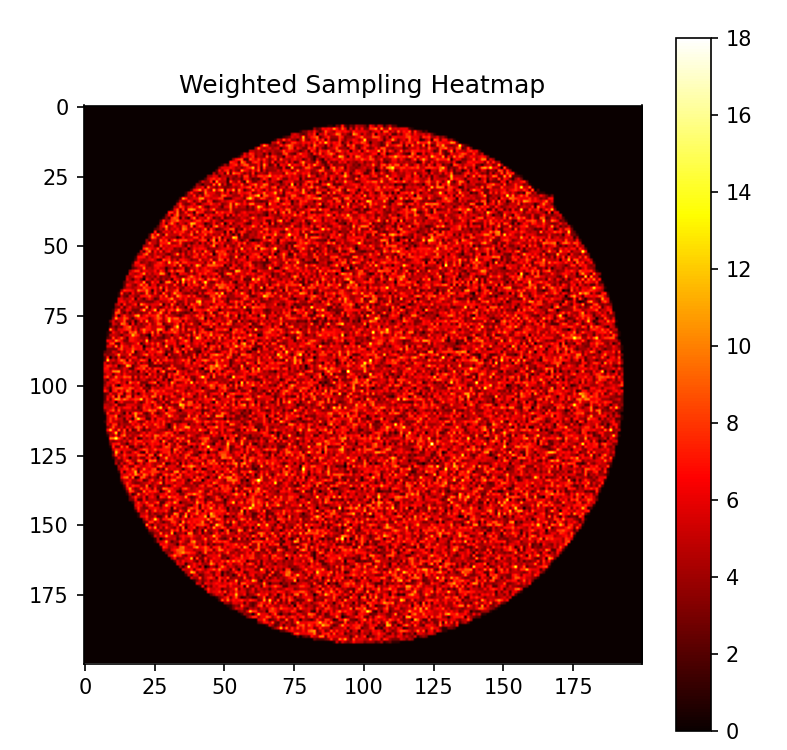
\includegraphics[width=\textwidth]{imaxes/muestraje/random_sampling_heatmap.png}
        \caption{Mapa de calor de mostraxe aleatoria}
        \label{fig:random_sampling_heatmap}
    \end{subfigure}
    \hfill
    \begin{subfigure}[b]{0.3\textwidth}
        \centering
        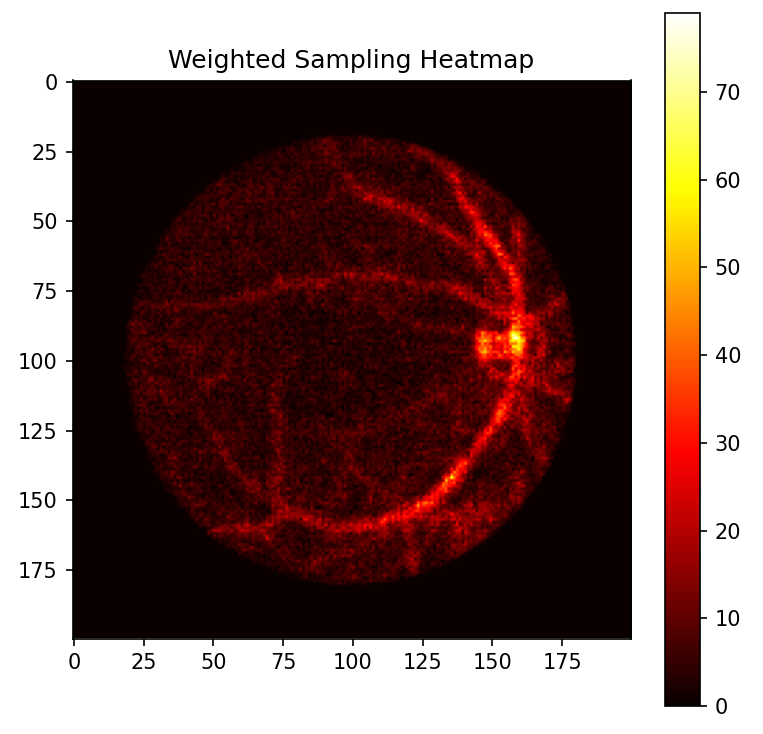
\includegraphics[width=\textwidth]{imaxes/muestraje/weighted_sampling_heatmap.png}
        \caption{Mapa de calor de mostraxe ponderada}
        \label{fig:weighted_sampling_heatmap}
    \end{subfigure}
    \hfill
    \begin{subfigure}[b]{0.3\textwidth}
        \centering
        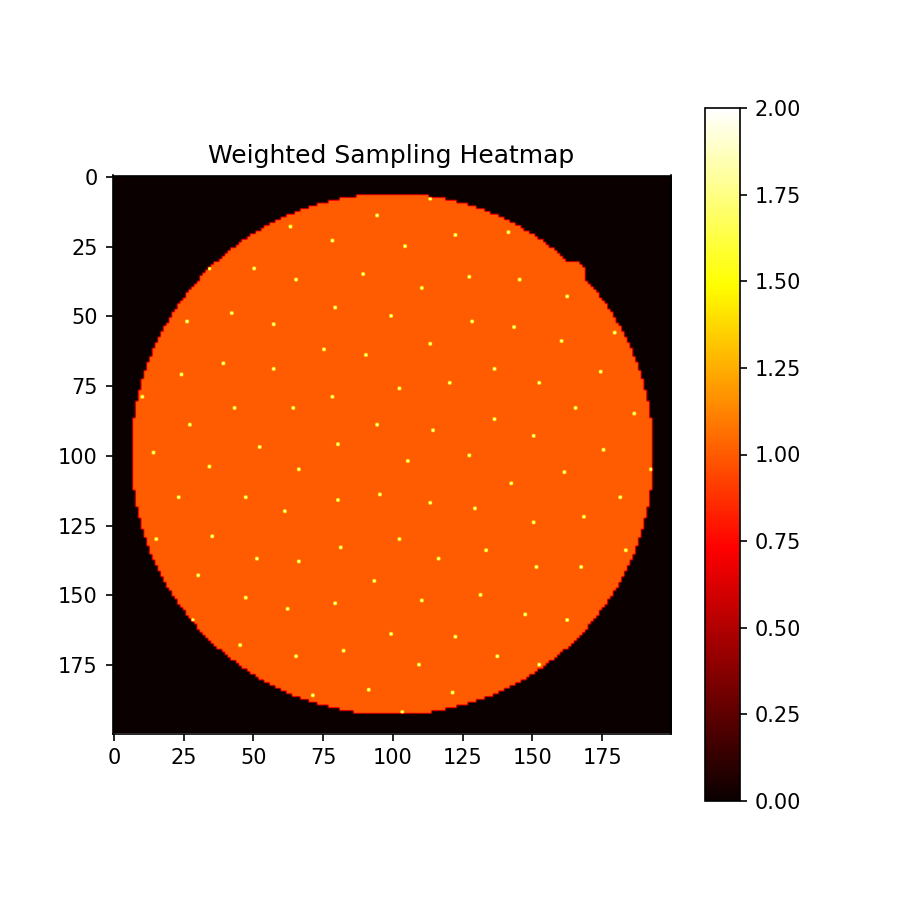
\includegraphics[width=\textwidth]{imaxes/muestraje/uniform_sampling_heatmap.png}
        \caption{Mapa de calor de mostraxe uniforme (100 puntos)}
        \label{fig:uniform_sampling_heatmap}
    \end{subfigure}
    \caption{Mapas de calor que ilustran as diferentes estratexias de mostraxe implementadas.}
    \label{fig:sampling_heatmaps}
\end{figure}

\subsubsection{Lotería de Inicialización}
\label{subsubsec:loteria_inicializacion}
Outra metodoloxía deseñada foi a implementación da lotería de inicialización. Esta técnica consiste en probar diferentes inicializacións aleatorias dos pesos da rede para determinar cal delas resulta máis beneficiosa para a converxencia e o rendemento final do modelo, e selecionar a mellor inicialización para completar o adestramento

\subsubsection{Axuste Dinámico do Tamaño do Lote}
\label{subsubsec:axuste_dinamico_batch_size}
Implementouse o axuste dinámico do tamaño do lote, que consiste en aumentar o `batch size` ao longo do adestramento. Para levar a cabo esta estratexia, divídense as épocas (epochs) en diferentes fases, onde cada fase fai uso dun tamaño de lote diferente, comezando normalmente con tamaños máis pequenos e aumentándoos progresivamente.



\section{Métodos de Avaliación}
\label{sec:Métodos de Avaliación}

A avaliación do rendemento do sistema de rexistro constitúe un aspecto fundamental para determinar a eficacia das modificacións implementadas. 
O proceso de avaliación divídese en dous enfoques complementarios: a avaliación cuantitativa, que emprega métricas numéricas obxectivas, e a avaliación cualitativa, que analiza os resultados de forma visual para detectar artefactos ou deformacións non desexadas que poidan escapar ás métricas numéricas.

 Ambas avaliacións son necesarias para obter unha visión completa da calidade do rexistro, xa que a avaliación cuantitativa pode non ser suficiente para detectar problemas visuais que non se reflictan nas métricas.

 \subsection{Avaliación Cuantitativa}
 \label{subsec:Avaliación Cuantitativa}
 
 Utilizamos como método de evaluación cuantitativa o proposto por FIRE \cite{FIRE}
 xerando un gráfico onde o eixo x representa o valor do límite de erro e o eixo y mostra a porcentaxe de pares de imaxes que foron rexistrados con éxito para cada límite de erro.
 
O erro de rexistro calcúlase mediante a distancia euclidiana media entre os puntos correspondentes nas imaxes fixa e móbil:

\begin{figure}[tbp]
    \centering
    \[
    E = \frac{1}{N} \sum_{i=1}^{N} \left\| p_i^{\text{fixo}} - T(p_i^{\text{móbil}}) \right\|
    \]
    \caption{Cálculo do erro de rexistro mediante a distancia euclidiana.}
    \label{fig:erro_registro}
\end{figure}

onde N é o número de puntos de referencia, p son as coordenadas dos puntos e T é a transformación aplicada.

Cando o erro de rexistro entre un par de imaxes está por debaixo do limiar, considérase que o rexistro foi exitoso e viceversa. Isto dá lugar a unha curva monótona e continua que reflicte a relación entre a taxa de éxito e a precisión obxectivo, evitando así a necesidade de establecer un limiar arbitrario. 
Estes gráficos utilízanse para ilustrar a precisión do rexistro tanto para casos individuais (onde se utilizan o porcentaxe de parellas de puntos rexistrados con éxito)
como para o conxunto completo de datos.
Esta métrica facilita a comparación entre distintos métodos competidores e permite seleccionar o máis axeitado segundo a precisión desexada.
 
Ademais, en FIRE a avaliación segmentarase nas 3 categorías de imaxes (S, P e A) para analizar o rendemento do rexistro en cada unha delas, xa que cada categoría presenta diferentes desafíos e características.

 Mentres que FIRE xa provee os puntos de referencia para a avaliación, RFMID non o fai.
 Polo tanto, para RFMID, utilizamos o mesmo método de avaliación, pero xerándo os puntos manualmente de forma que cubran o interior da máscara da imaxe fixa (separados por 50 píxeles entre si).
 
 \begin{figure}[tbp]
    \centering
    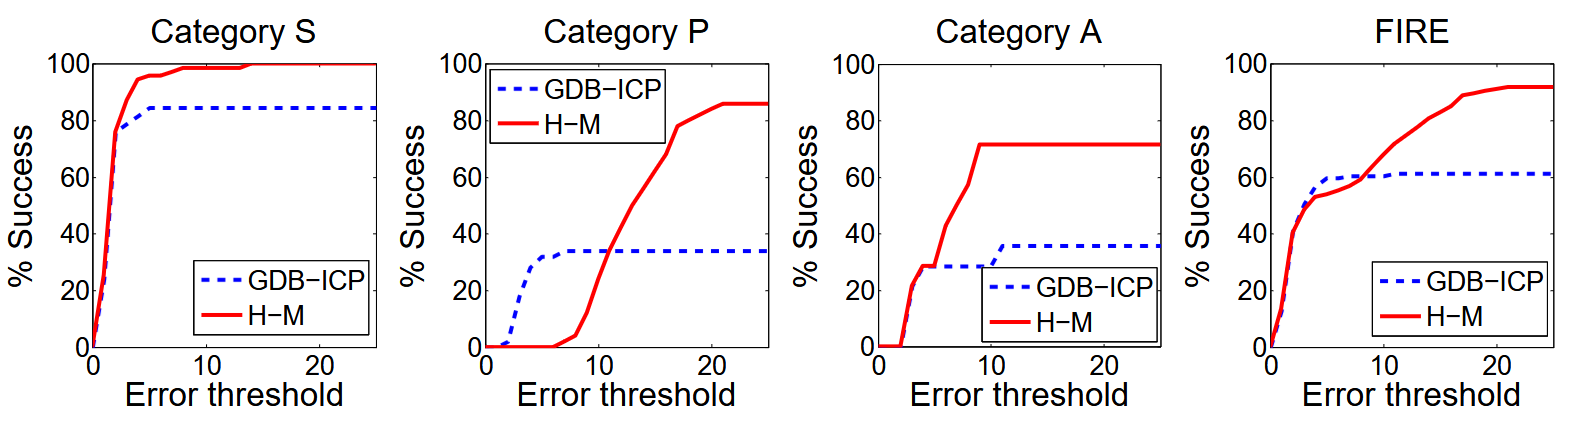
\includegraphics[width=0.8\textwidth]{imaxes/fire_aval.png}
    \caption{Gráfico de avaliación FIRE \cite{FIRE}}
    \label{fig:fire_aval}
\end{figure}

No caso de RFMiD, dividiremos o conxunto de datos en varias categorías dependendo da dificultade do rexistro, que se calcula mediante a norma de Frobenius dunha matriz $A \in \mathbb{R}^{m \times n}$.
Esta é unha xeralización da distancia euclidiana aplicada a matrices, onde as imaxes con transformacións mais grandes considéranse mais difíciles.

\begin{figure}[tbp]
    \centering
    \[
    \|A\|_F = \sqrt{\sum_{i=1}^{m} \sum_{j=1}^{n} |a_{ij}|^2}
    \]
    \caption{Norma de Frobenius dunha matriz $A \in \mathbb{R}^{m \times n}$, onde $a_{ij}$ son os elementos da matriz $A$.}
    \label{fig:frobenius_norm}
\end{figure}

Nalgúns casos temén utilizaremos a distancia media entre os puntos correspondentes como métrica complementaria para avaliar a calidade do rexistro, xa que a taxa de éxito pode non ser suficiente para detectar os cambios.

\subsection{Avaliación Cualitativa}
\label{subsec:Avaliación Cualitativa}

No caso deste traballo, a avaliación cualitativa cobra gran importancia, xa que na cuantitativa so se está a comparar sobre un número reducido de puntos en cada parexa de imaxes.
A avaliación visual permite detectar problemas que non se reflictan nas métricas cuantitativas, como artefactos visuais ou deformacións non desexadas, 
especialmente en rexistros que teñen deformacións locais que poden non coincidir con ningún punto.

No caso do dataset FIRE \cite{FIRE}, a avaliación visual é especialmente relevante, xa que tan só se proporcionan 10 puntos de referencia por imaxe, que poden non ser suficientes para avaliar a calidade do rexistro en moitas zonas da imaxe.
Xa que en RFMID \cite{RFMiD} utilízanse puntos de referencia xerados manualmente que cubren toda a imaxe, a avaliación visual é algo menos relevante, xa que é máis probable que unha deformación local incorrecta sexa detectada por algún punto e se vexa reflexado nas métricas.

Co obxetivo de identificar facilmente os distintos artefactos visuais ou transformación non realista, utilízanse diferentes ferramentas como a composición de imaxes, a visualización dos vectores de desprazamento e a comparación de imaxes antes e despois do rexistro.
Na figura \ref{fig:visex} pódense observar algúns exemplos de estas.

\begin{figure}[tbp]
    \centering
    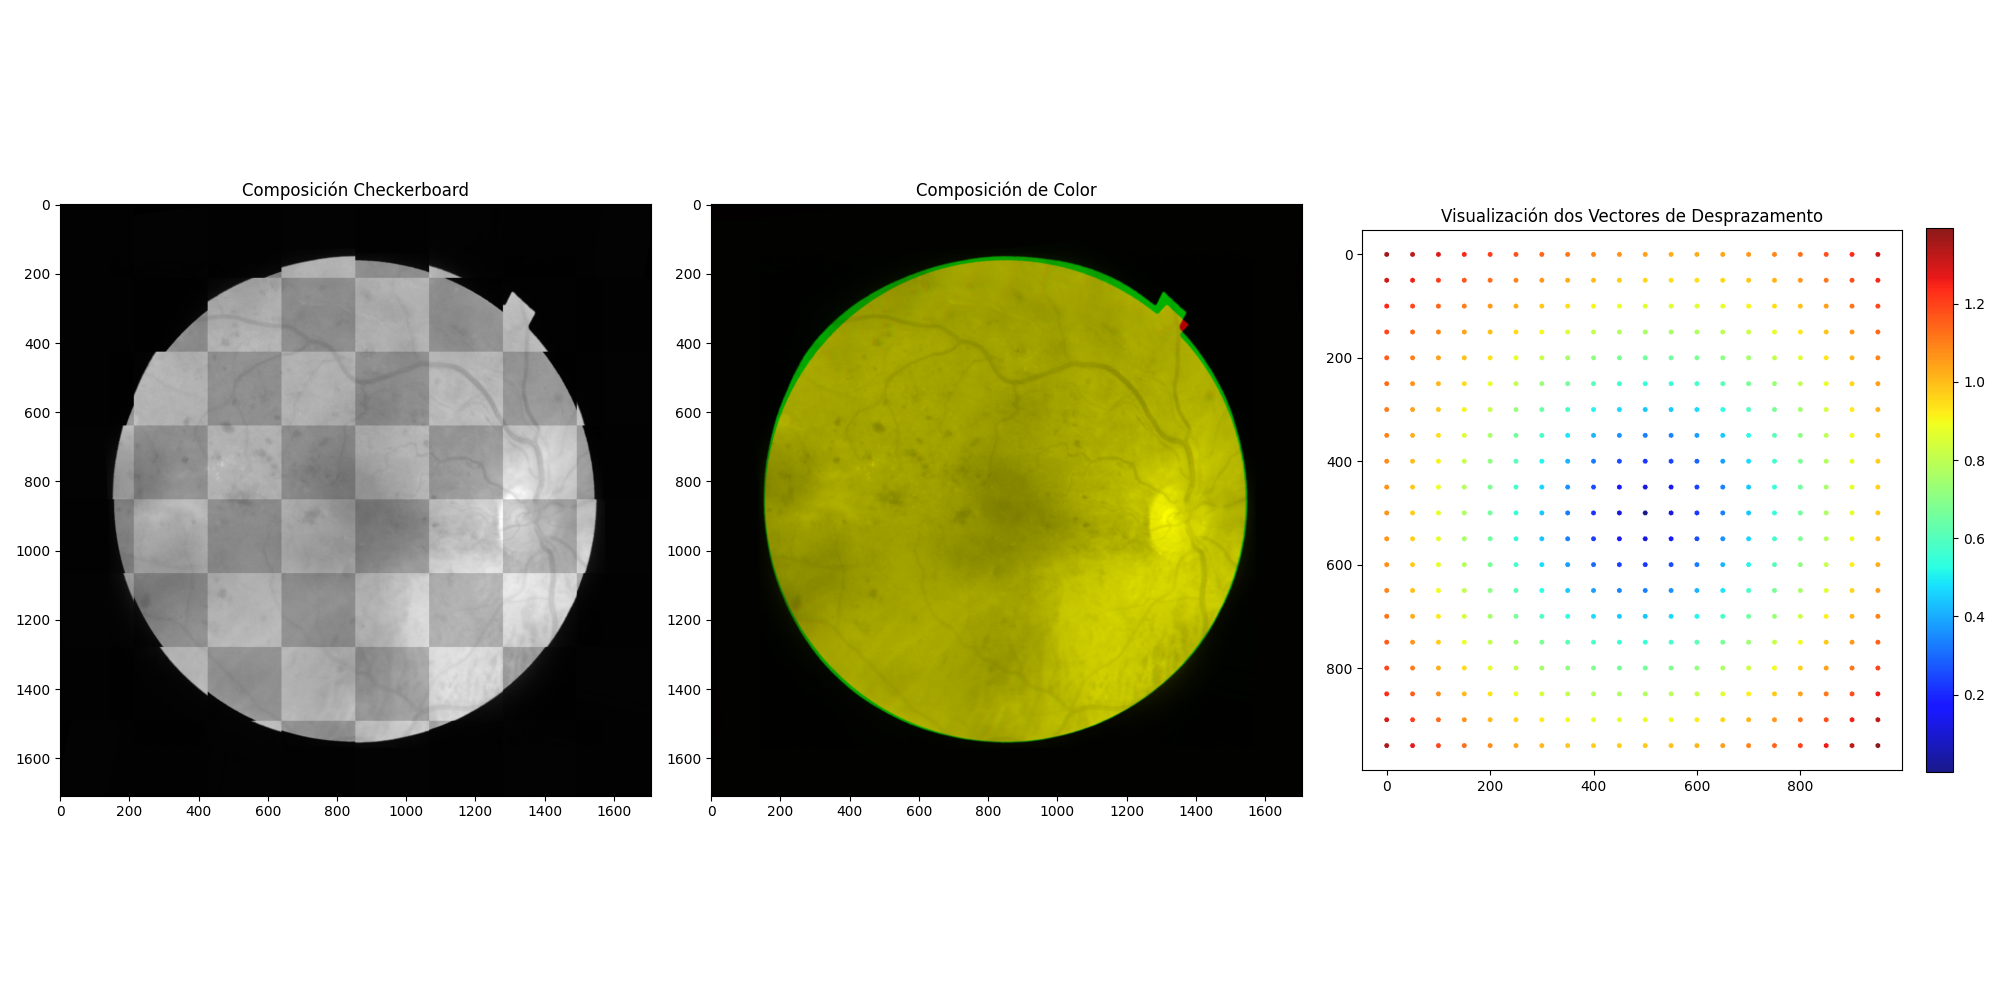
\includegraphics[width=0.9\textwidth]{imaxes/visex.png}
    \caption{Exemplos de avaliación visual: (a) Composición de imaxes en checkerboard, (b) Composición de imaxes por cor, (c) Visualización dos vectores de desprazamento.}
    \label{fig:visex}
\end{figure}
 \chapter{Experimentos e resultados}
\label{chap:Experimentos e resultados}
\lettrine{N}{este} capítulo presentaranse os experimentos realizados e os resultados obtidos.
Para iso, comezarase presentando unha vista xeral do proceso de experimentación, 
seguido dos propios experimentos realizados, para 
Finalmente analizar os resultados obtidos en conxunto e as conclusións que se poden extraer deles.

\section{Vista Xeral}
\label{sec:Vista Xeral}

O obxetivo do traballo é determinar se as redes implícitas son aptas para a tarefa de rexistro de retinas.
Aínda que partimos do traballo de IDIR, a tarefa de rexistro de retinas presenta diferenzas importantes respecto ao rexistro de pulmóns. Por este motivo, non podemos asumir que os parámetros óptimos para pulmóns sexan tamén os mellores para retinas.

Ao longo dos experimentos, a comparación principal céntrase na función de activación empregada (SIREN ou ReLU).
Debido ao gran espazo de búsqueda que implica probar todas as configuracións posibles, 
os experimentos iniciais centraránse en fixar unha unha seria de parámetros con valores razoables para poder experimentar só con aqueles que teñan un impacto máis significativo.

Ademais, debido ás diferencias entre as funcións de activación, é posible que cada unha require unha configuración diferente para obter os mellores resultados.
Por exemplo, o sesgo que SIREN ten cara sinais de alta frecuencia fará que o proceso de regularización sexa mais relevante para evitar o sobreaxuste.

\section{Experimentos}
\label{sec:Experimentos}

\subsection{Experimentos iniciais}
\label{subsec:Experimentos iniciais}

Inicialmente tentaremos determinar uns valores aceptables para varios dos parámetros da rede.
Isto é relevante xa que moitos destes parámetros son dependentes uns de outros.

A menos que especificado de outro xeito, os parámetros utilizados para os experimentos son os seguintes:
\begin{itemize}
    \item Función de perda: NCC
    \item Regularización:
    \begin{itemize}
         \item Bending energy penalty: 10.0
         \item Jacobian regularizer: 0.05
         \item Hyperelastic regularizer: 0.25
    \end{itemize}
    \item Learning rate: 0.0001
    \item Batch size: 10000 puntos
    \item Epochs: 1500
    \item Optimizador: Adam
    \item Resolución: 1000x1000
\end{itemize}


\subsubsection{Función de loss}
\label{subsubsec:Función de loss}

\paragraph{Planteamento}
\label{par:Planteamento-loss}

A función de loss é un dos aspectos máis importantes á hora de entrenar unha rede neuronal.
As funcións de perda valoradas para este traballo xa forón explicadas en \ref{subsubsec:Termos de loss}.

Para determinar cal é a función de perda mais adecuada para a tarefa de rexistro de retinas, realizáronse experimentos comparando o rendemento de cada unha sobre unha mostra de imaxes dos datases de FIRE e RFMID.
Xa que a rede non é capaz de rexistrar con éxito a gran parte das imaxes, tomaráse a distancia media de todos os puntos como métrica de comparación.

\paragraph{Resultados}
\label{par:Resultados-loss}

Os resultados obtidos son os seguintes: \ref{tab:mean_distances}, \ref{fig:loss_functions_comparison}

% \begin{table}[h]
%     \centering
%     \begin{tabular}{|l|c|c|}
%     \hline
%     Loss Function & FIRE Mean Distance & RFMID Mean Distance \\ \hline
%     ncc & 250.59 & 36.04 \\ \hline
%     mse & 392.94 & 9.50 \\ \hline
%     l1 & 404.83 & 5.42 \\ \hline
%     smoothl1 & 414.79 & 7.01 \\ \hline
%     \end{tabular}
%     \caption{Distancias medias según a función de perda. Valores máis baixos son mellores.}
%     \label{tab:mean_distances}
% \end{table}


\begin{table}[ht]
    \centering
    \begin{tabular}{|l|cc|cc|}
    \hline
    \multirow{2}{*}{Loss Function} & \multicolumn{2}{c|}{FIRE Dataset} & \multicolumn{2}{c|}{RFMID Dataset} \\ \cline{2-5}
     & Relu & SIREN & Relu & SIREN \\ \hline
    huber & 399.86 & 397.45 & 7.13 & 57.31 \\ \hline
    l1 & 404.83 & 391.87 & 5.42 & 52.91 \\ \hline
    mse & 392.94 & 410.97 & 9.50 & 121.54 \\ \hline
    ncc & 250.59 & 281.03 & 36.04 & 79.84 \\ \hline
    smoothl1 & 414.79 & 387.71 & 7.01 & 60.74 \\ \hline
    ssim & 268.72 & 264.98 & 23.34 & 55.07 \\ \hline
    \end{tabular}
    \caption{Distancias medias segundo función de perda, tipo de rede e datasets (FIRE vs. RFMID)}
    \label{tab:mean_distances}
\end{table}

\begin{figure}[ht]
    \centering
    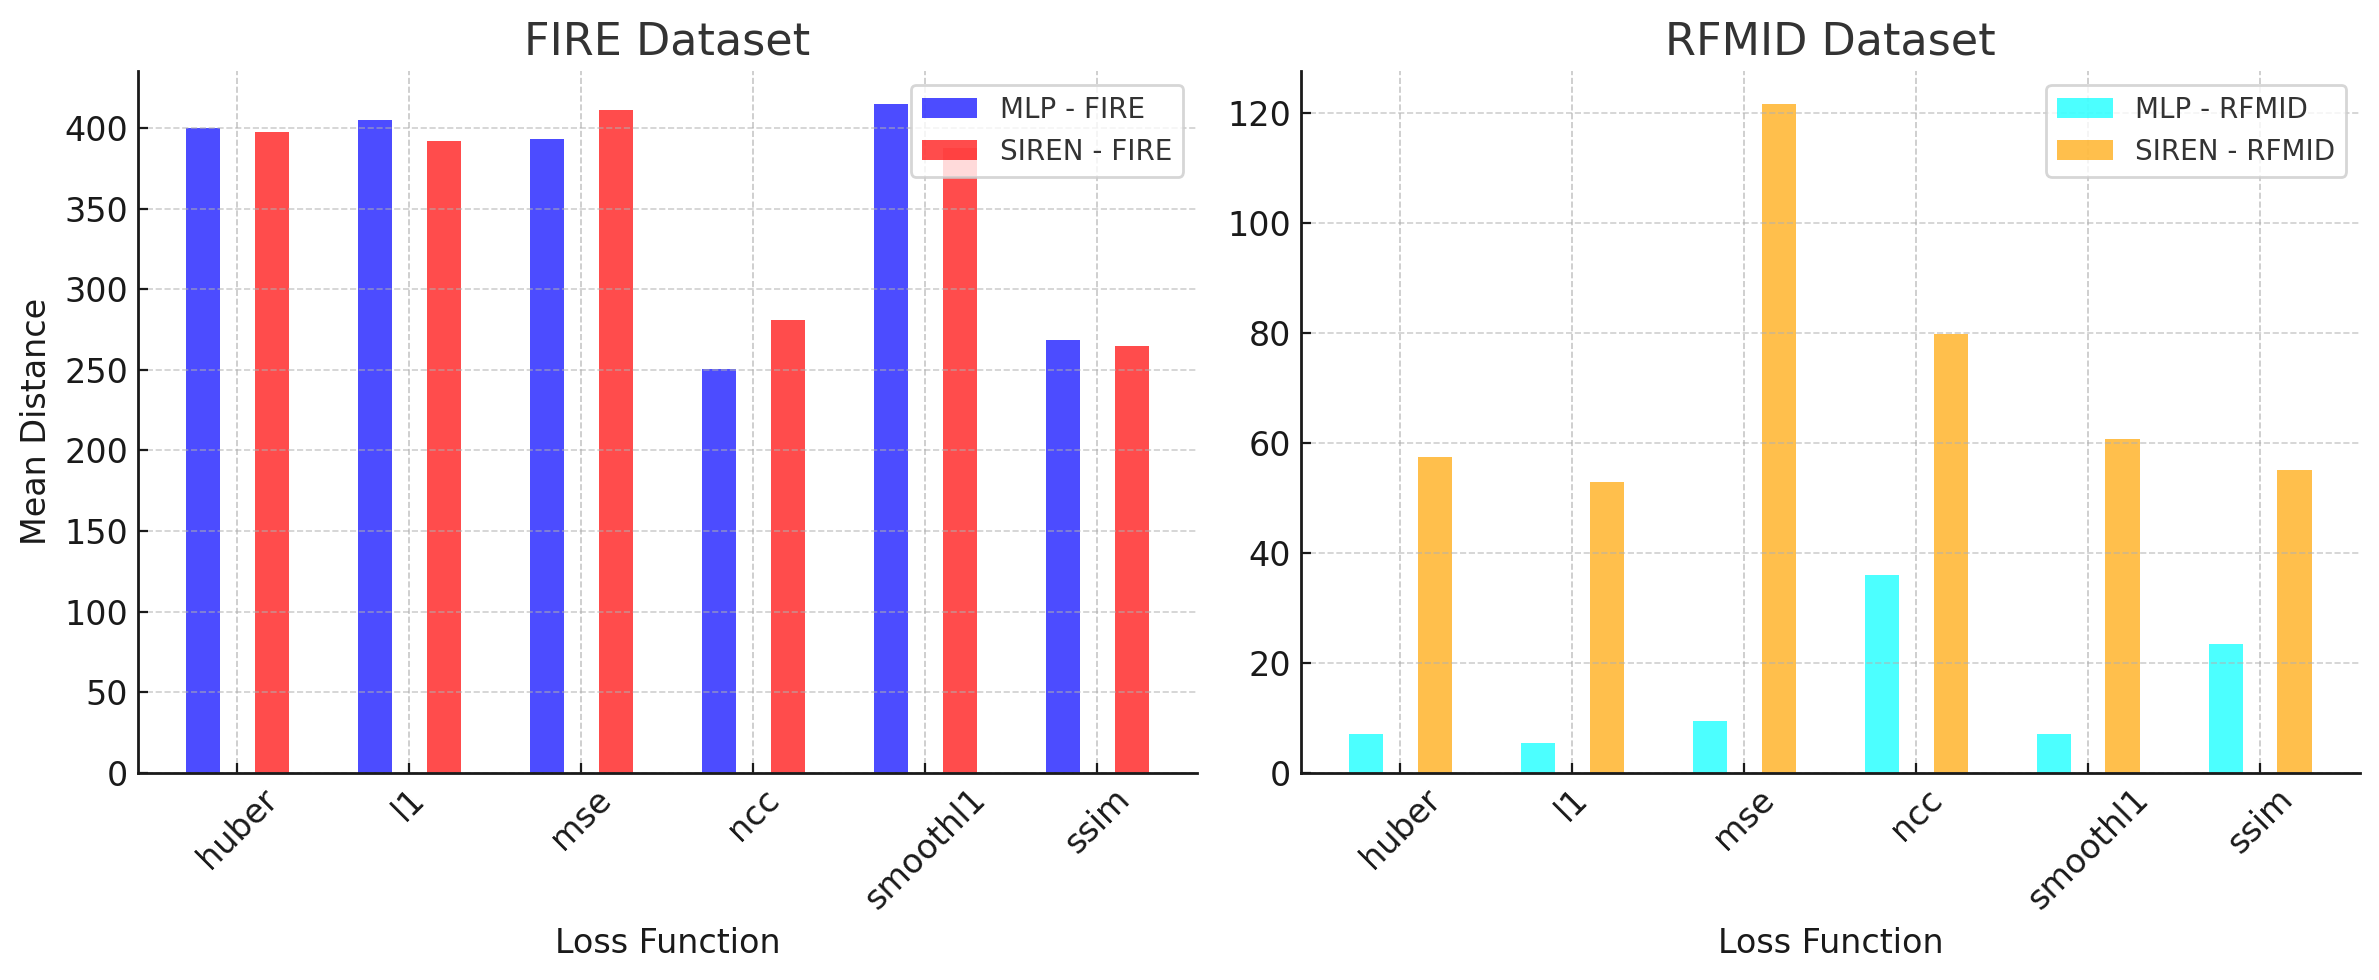
\includegraphics[width=0.75\textwidth]{imaxes/losstype.png}
    \caption{Comparación de diferentes funcións de perda sobre imaxes de FIRE e RFMID}
    \label{fig:loss_functions_comparison}
\end{figure}
    


\paragraph{Discusión}
\label{par:Discusion-loss}

Obsérvase como as métricas que teñen en conta a estructura da imaxe (NCC, SSIM) tenden a dar mellores resultados que aquelas que non o fan (MSE, Huber, Smooth L1) co dataset de FIRE, mentres que con RFMID ocurre ó contrario.
Isto pode deberse a que as imaxes reais de retina teñen unha maior variabilidade na iluminación e contraste, polo que as métricas que non teñen en conta a estructura da imaxe serán menos robustas a estas diferenzas.
No caso de RFMID, ao ser imaxes sintéticas, a variabilidade na iluminación e contraste é nula, o que explica os mellores resultados das métricas que non teñen en conta a estructura da imaxe.

NCC tende a ser mais robusta a combios uniformes na intensidade global, mentres que SSIM tende a ser mellor con cambios locais.
SSIM tamén é menos robusta ao ruído, sensible o tamaño das seccións utilizadas e computacionalmente mais costosa. Ademais, ten outro custo engadido xa que non é posible calcular SSIM tan só comparando os puntos mostrados xa que utiliza xanelas deslizantes para evaluar luminancia, contraste e estrutura. 
Para utilizala é necesario reconstruir a imaxen en cada iteracion o que ten un alto custo computacional.
No caso de non reconstruir a imaxe e utilizar os puntos mostrados directamente, esta métrica funciona igualmente mais con resultados lixeiramente peores, xa que perde toda a súa capacidade de capturar variacións locais de luminancia, contraste e estrutura, o que se tradúce nunha función de perda global sen consideraciós locais.

\paragraph{Conclusións}
\label{par:Conclusions-loss}

En base aos resultados obtidos, pódense extraer varias conclusións relevantes:

1. Para o dataset FIRE, que contén imaxes reais de retina con variabilidade en iluminación e contraste, as funcións de perda baseadas en características estruturais como NCC e SSIM proporcionan resultados significativamente mellores. En particular, NCC mostra o menor erro medio (250.59 para Relu e 281.03 para SIREN).
2. Para o dataset RFMID, que contén imaxes con tan só variación xeométrica, as funcións de perda baseadas en píxeles como L1 e Smooth L1 ofrecen mellores resultados. Concretamente, L1 presenta o menor erro medio para Relu (5.42) e resultados competitivos para SIREN (52.91).
3. Obsérvase unha diferenza sistemática entre os modelos Relu e SIREN, sendo os primeiros máis efectivos para o dataset RFMID, mentres que ambos mostran rendementos comparables para FIRE. Isto débese a que Relu tende a producir funcións predominantemente lineares, o que se adapta mellor ás transformacións realizadas no dataset RFMID.
4. SSIM, a pesar de ser teoricamente robusta a cambios locais, non mostra unha vantaxe significativa sobre NCC.

A elección de NCC como función de perda estándar baséase tanto na súa robustez empírica coma na súa consistencia co obxectivo de alinear imaxes reais de retina, onde a variabilidade en iluminación e contraste é un factor importante.

\subsubsection{Resolución da imaxe}
\label{subsubsec:Resolución da imaxe}

\paragraph{Planteamento}
\label{par:Planteamento-resolution}

A resolución da imaxe é un aspecto clave xa que inflúe de forma directa no resto de parámetros da rede.
Por exemplo, un batch size de 1000 puntos nunha imaxe de 256x256 é unha densidade de puntos moito maior que nunha imaxe de 512x512.

Ademais, a resolución da imaxe tamén inflúe na capacidade da rede para aprender as transformacións, xa que a información que recibe é mais detallada. 
Isto pode ser beneficioso se estos detalles conteñen información relevante para a tarefa de rexistro, pero tamén podería ser perxudicial se conteñen unha gran parte de ruido.

O tamaño das imaxes tamén é unha das principais diferencias entre as imaxes de retina e as de pulmóns utilizadas orixinalmente por IDIR, tendo estas últimas de 512x512 mentres que as imaxes dos ollos contan con resolucións de ata 2160x2160.

Para determinar cal é a resolución mais adecuada, realizáronse experimentos comparando o rendemento de cada unha sobre unha mostra de imaxes dos datases de FIRE e RFMID.
Debido a que a rede non é capaz de rexistrar con éxito a gran parte das imaxes, tomaráse a distancia media de todos os puntos como métrica de comparación.

\paragraph{Resultados}
\label{par:Resultados-resolution}

\ref{tab:mlp_mean_distances_fire}, \ref{tab:siren_mean_distances_fire}, \ref{tab:mlp_mean_distances_rfmid}, \ref{tab:siren_mean_distances_rfmid}

\begin{table}[h]
    \centering
    \begin{minipage}[t]{0.45\linewidth}
        \centering
        \begin{tabular}{|c|c|}
        \hline
        Resolution & Mean Distance \\ \hline
        100 & 254.22 \\ \hline
        250 & 251.29 \\ \hline
        750 & 250.62 \\ \hline
        1250 & 250.59 \\ \hline
        1708 & 249.72 \\ \hline
        \end{tabular}
        \caption{Distancias medias para o dataset FIRE ca función de activación Relu}
        \label{tab:mlp_mean_distances_fire}
    \end{minipage}
    \hfill
    \begin{minipage}[t]{0.45\linewidth}
        \centering
        \begin{tabular}{|c|c|}
        \hline
        Resolution & Mean Distance \\ \hline
        100 & 266.43 \\ \hline
        250 & 263.85 \\ \hline
        750 & 263.19 \\ \hline
        1250 & 258.56 \\ \hline
        1708 & 258.06 \\ \hline
        \end{tabular}
        \caption{Distancias medias para o dataset FIRE ca función de activación SIREN}
        \label{tab:siren_mean_distances_fire}
    \end{minipage}
\end{table}

\begin{table}[h]
    \centering
    \begin{minipage}[t]{0.45\linewidth}
        \centering
        \begin{tabular}{|c|c|}
        \hline
        Resolution & Mean Distance \\ \hline
        100 & 37.29 \\ \hline
        250 & 36.18 \\ \hline
        750 & 36.01 \\ \hline
        1250 & 35.03 \\ \hline
        1708 & 35.04 \\ \hline
        \end{tabular}
        \caption{Distancias medias para o dataset RFMID ca función de activación Relu}
        \label{tab:mlp_mean_distances_rfmid}
    \end{minipage}
    \hfill
    \begin{minipage}[t]{0.45\linewidth}
        \centering
        \begin{tabular}{|c|c|}
        \hline
        Resolution & Mean Distance \\ \hline
        100 & 68.12 \\ \hline
        250 & 73.42 \\ \hline
        750 & 77.55 \\ \hline
        1250 & 67.33 \\ \hline
        1708 & 67.31 \\ \hline
        \end{tabular}
        \caption{Distancias medias para o dataset RMIFD ca función de activación SIREN}
        \label{tab:siren_mean_distances_rfmid}
    \end{minipage}
\end{table}

\paragraph{Discusión}
\label{par:Discusion-resolution}

Pódese observar como unha maior resolución tende a dar lixeiramente mellores resultados, pero a un custo computacional maior.
Isto pode deberse mais á precisión ca que se fai a evaluación mais que a unha mellor capacidade da rede para aprender as transformacións, xa que as diferencias son moi pequenas e consistentes entre os diferentes parellas de imaxes.
Isto suxire que a resolución non ten un impacto significativo no rendemento da rede, e que a maioría da información relevante para a tarefa de rexistro xa está capturada en resolucións inferiores.


\paragraph{Conclusións}
\label{par:Conclusions-resolution}

Baseándonos nos resultados obtidos, podemos concluír que:

1. Resolucións inferiores a 100×100 non capturan suficientes detalles das estruturas vasculares retinianas para realizar un rexistro preciso, especialmente en imaxes reais do dataset FIRE.

2. Aumentar a resolución por encima de 1250x1250 non aporta beneficios significativos.

3. O comportamento respecto á resolución é consistente para ambos tipos de modelos (Relu e SIREN) e para ambos datasets (FIRE e RFMID), o que suxire que estas conclusións son xeneralizables.

Para os experimentos subseguintes, adoptarase unha resolución estándar de 1000x1000 píxeles, que demostrou proporcionar o mellor rendemento global para a tarefa de rexistro de retinas.

\subsubsection{Regularización}
\label{subsubsec:Regularización}

\paragraph{Planteamento}
\label{par:Planteamento-regularization}
O proceso de regularización axuda a rede a evitar o sobreaxuste, modificando o termo de loss para penalizar as transformacións pouco realistas.
As técnicas de regularización valoradas, que xa forón explicadas en detalle en \ref{subsubsec:Termos de regularización}, son as seguintes:

\begin{itemize}
    \item Regularizador do Jacobiano: penaliza as desviaciones do determinante da matriz Jacobiana respecto a 1, limitando expansións ou compresións locais excesivas.
    \item Regularizador hiperelástico: engade termos basados na enerxía de deformación, controlando a extensión e a expansión de superficie e garantindo transformacions suaves y difeomórficas.
    \item Penalización da enerxía de flexión: mide a magnitude das segundas derivadas do campo de deformación, promovendo que a superficie resultante sea o mais realista posible e reduciendo oscilacións de alta frecuencia.
\end{itemize}

Se os termos de regularización teñen demasiada influencia sobre o termo de loss, a rede fará transformacións moi pequenas para evitar ser penalizada, o que resultará nunha transformación insuficiente.
Por outro lado, se os termos son demasiado pequenos, a rede fará transformacións moi grandes, o que resulta nunha transformación irrealista e sobreaxustada. Isto é especialmente evidente no caso da función de activación SIREN, que tende a sobreaxustarse facilmente debido ao seu sesgo cara sinais de alta frecuencia.
A cantidade óptima de regularización depende da parexa concreta de imaxes a alinear, polo que intentaremos determinar cal é a mellor para unha mostra de imaxes.

A regularización tamén ten un impacto significativo no tempo de computación, xa que require múltiples pasadas de retropropagación por época para calcular os distintos termos de penalización.
Sen regularización só se fai 1 pasada para calcular o gradiente do termo de similitude da imaxe.
Ca regularización do Jacobiano, ademais do termo de similitude, calcúlanse dúas derivadas (unha por dimensión) para obter o Jacobiano, resultando en 3 pasadas por época.
Engadindo a regularización hiperelástica (sen termo de volume), é necesario calcular unha derivada adicional para o cofactor da matriz Jacobiana, facendo un total de 4 pasadas por época.
Finalmente, ca penalización de enerxía de flexión, necesitanse derivadas segundas, o que implica 7 pasadas por época en total.
Na traballo orixinal de IDIR, chegaban a usar 13 pasadas debido a que traballan en 3D.

Ademais, pese a que os diferentes termos de regularización valoran diferentes aspectos, cabe ter en conta que tamén coinciden nalgunhas das propiedades que valoran.
Por exemplo, o regularizador hiperelástico pode considerarse un caso mais xeral que inclúe indirectamente penalizaciones de volumen (Jacobian) e de suavidade (parte de la energía de flexión).

Para determinar cal é a regularización óptima, realizáronse experimentos comparando o rendemento de cada unha sobre unha mostra de imaxes dos datases de FIRE e RFMID cas diferentes funcións de activación.
Destes experimentos obterase un mapa de calor que mostra a distancia media entre os puntos correspondentes para cada combinación de parámetros.

\paragraph{Resultados}
\label{par:Resultados-regularization}

\ref{fig:gs_single_heatmaps}

\begin{figure}[ht]
    \centering
    \begin{subfigure}[b]{0.45\textwidth}
        \centering
        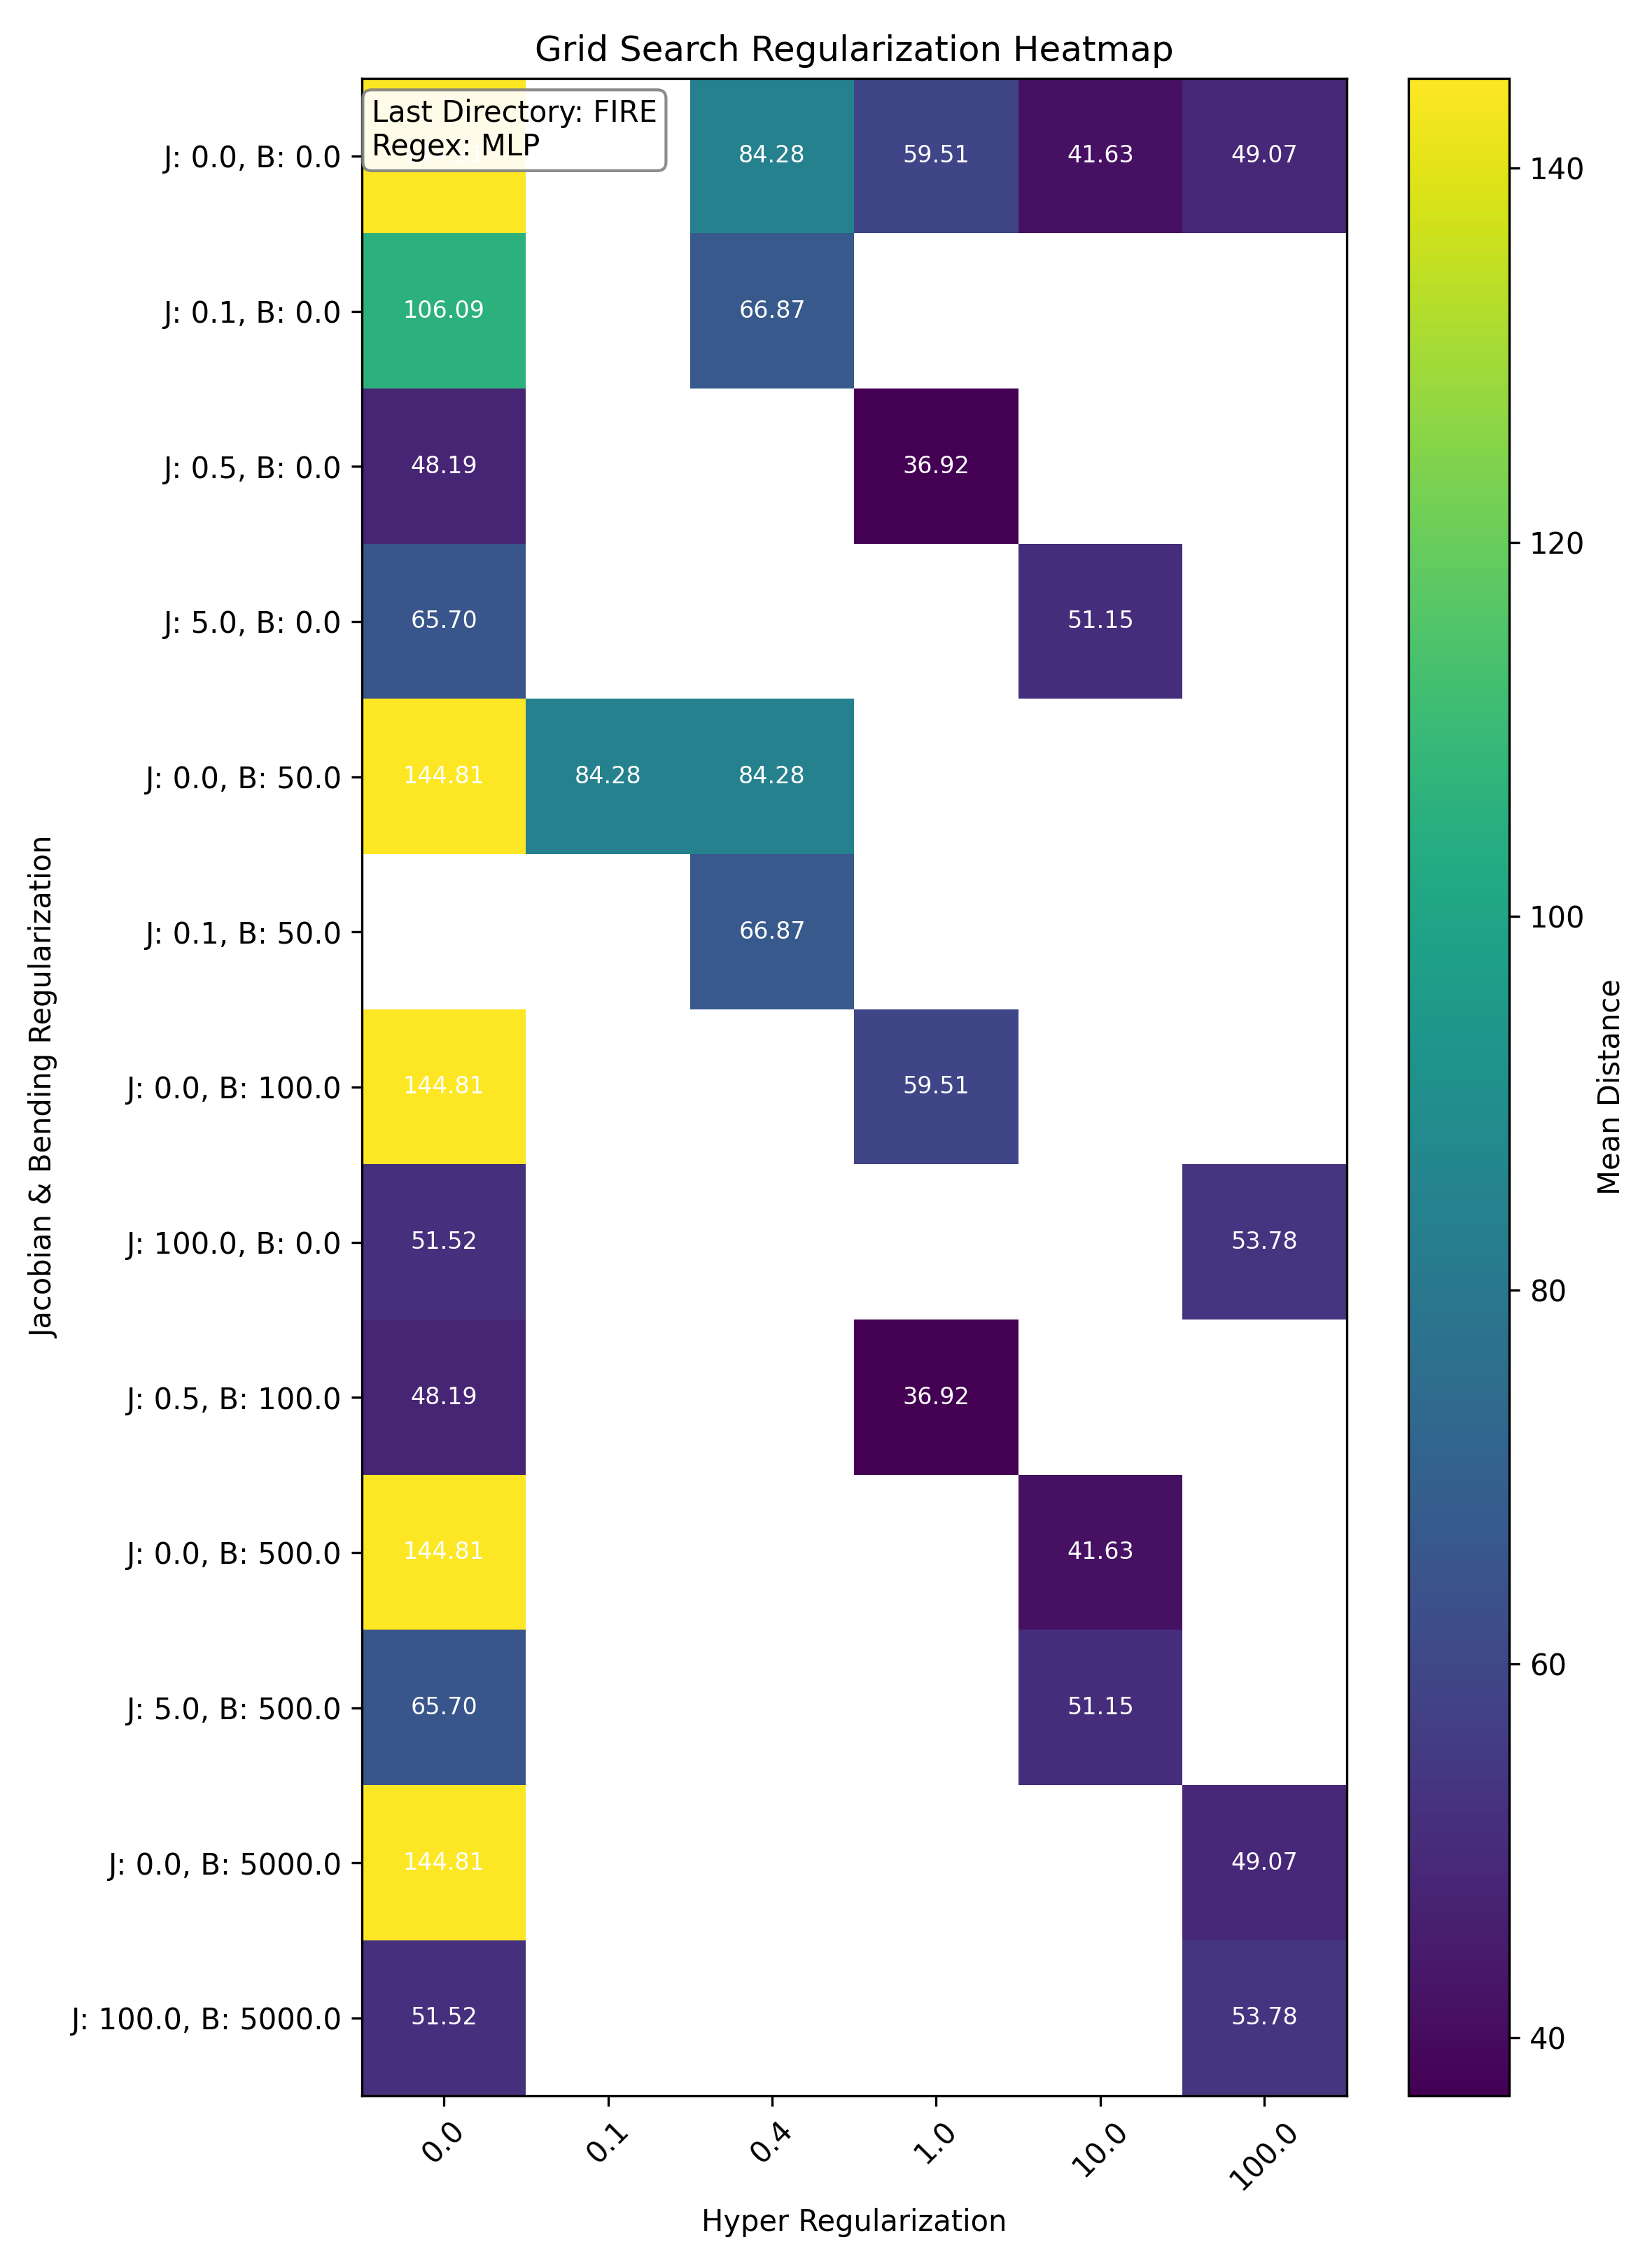
\includegraphics[width=\textwidth]{imaxes/grid_search_single_heatmap_FIRE_MLP.png}
        \caption{FIRE - Relu}
        \label{fig:gs_single_FIRE_MLP}
    \end{subfigure}\hfill
    \begin{subfigure}[b]{0.45\textwidth}
        \centering
        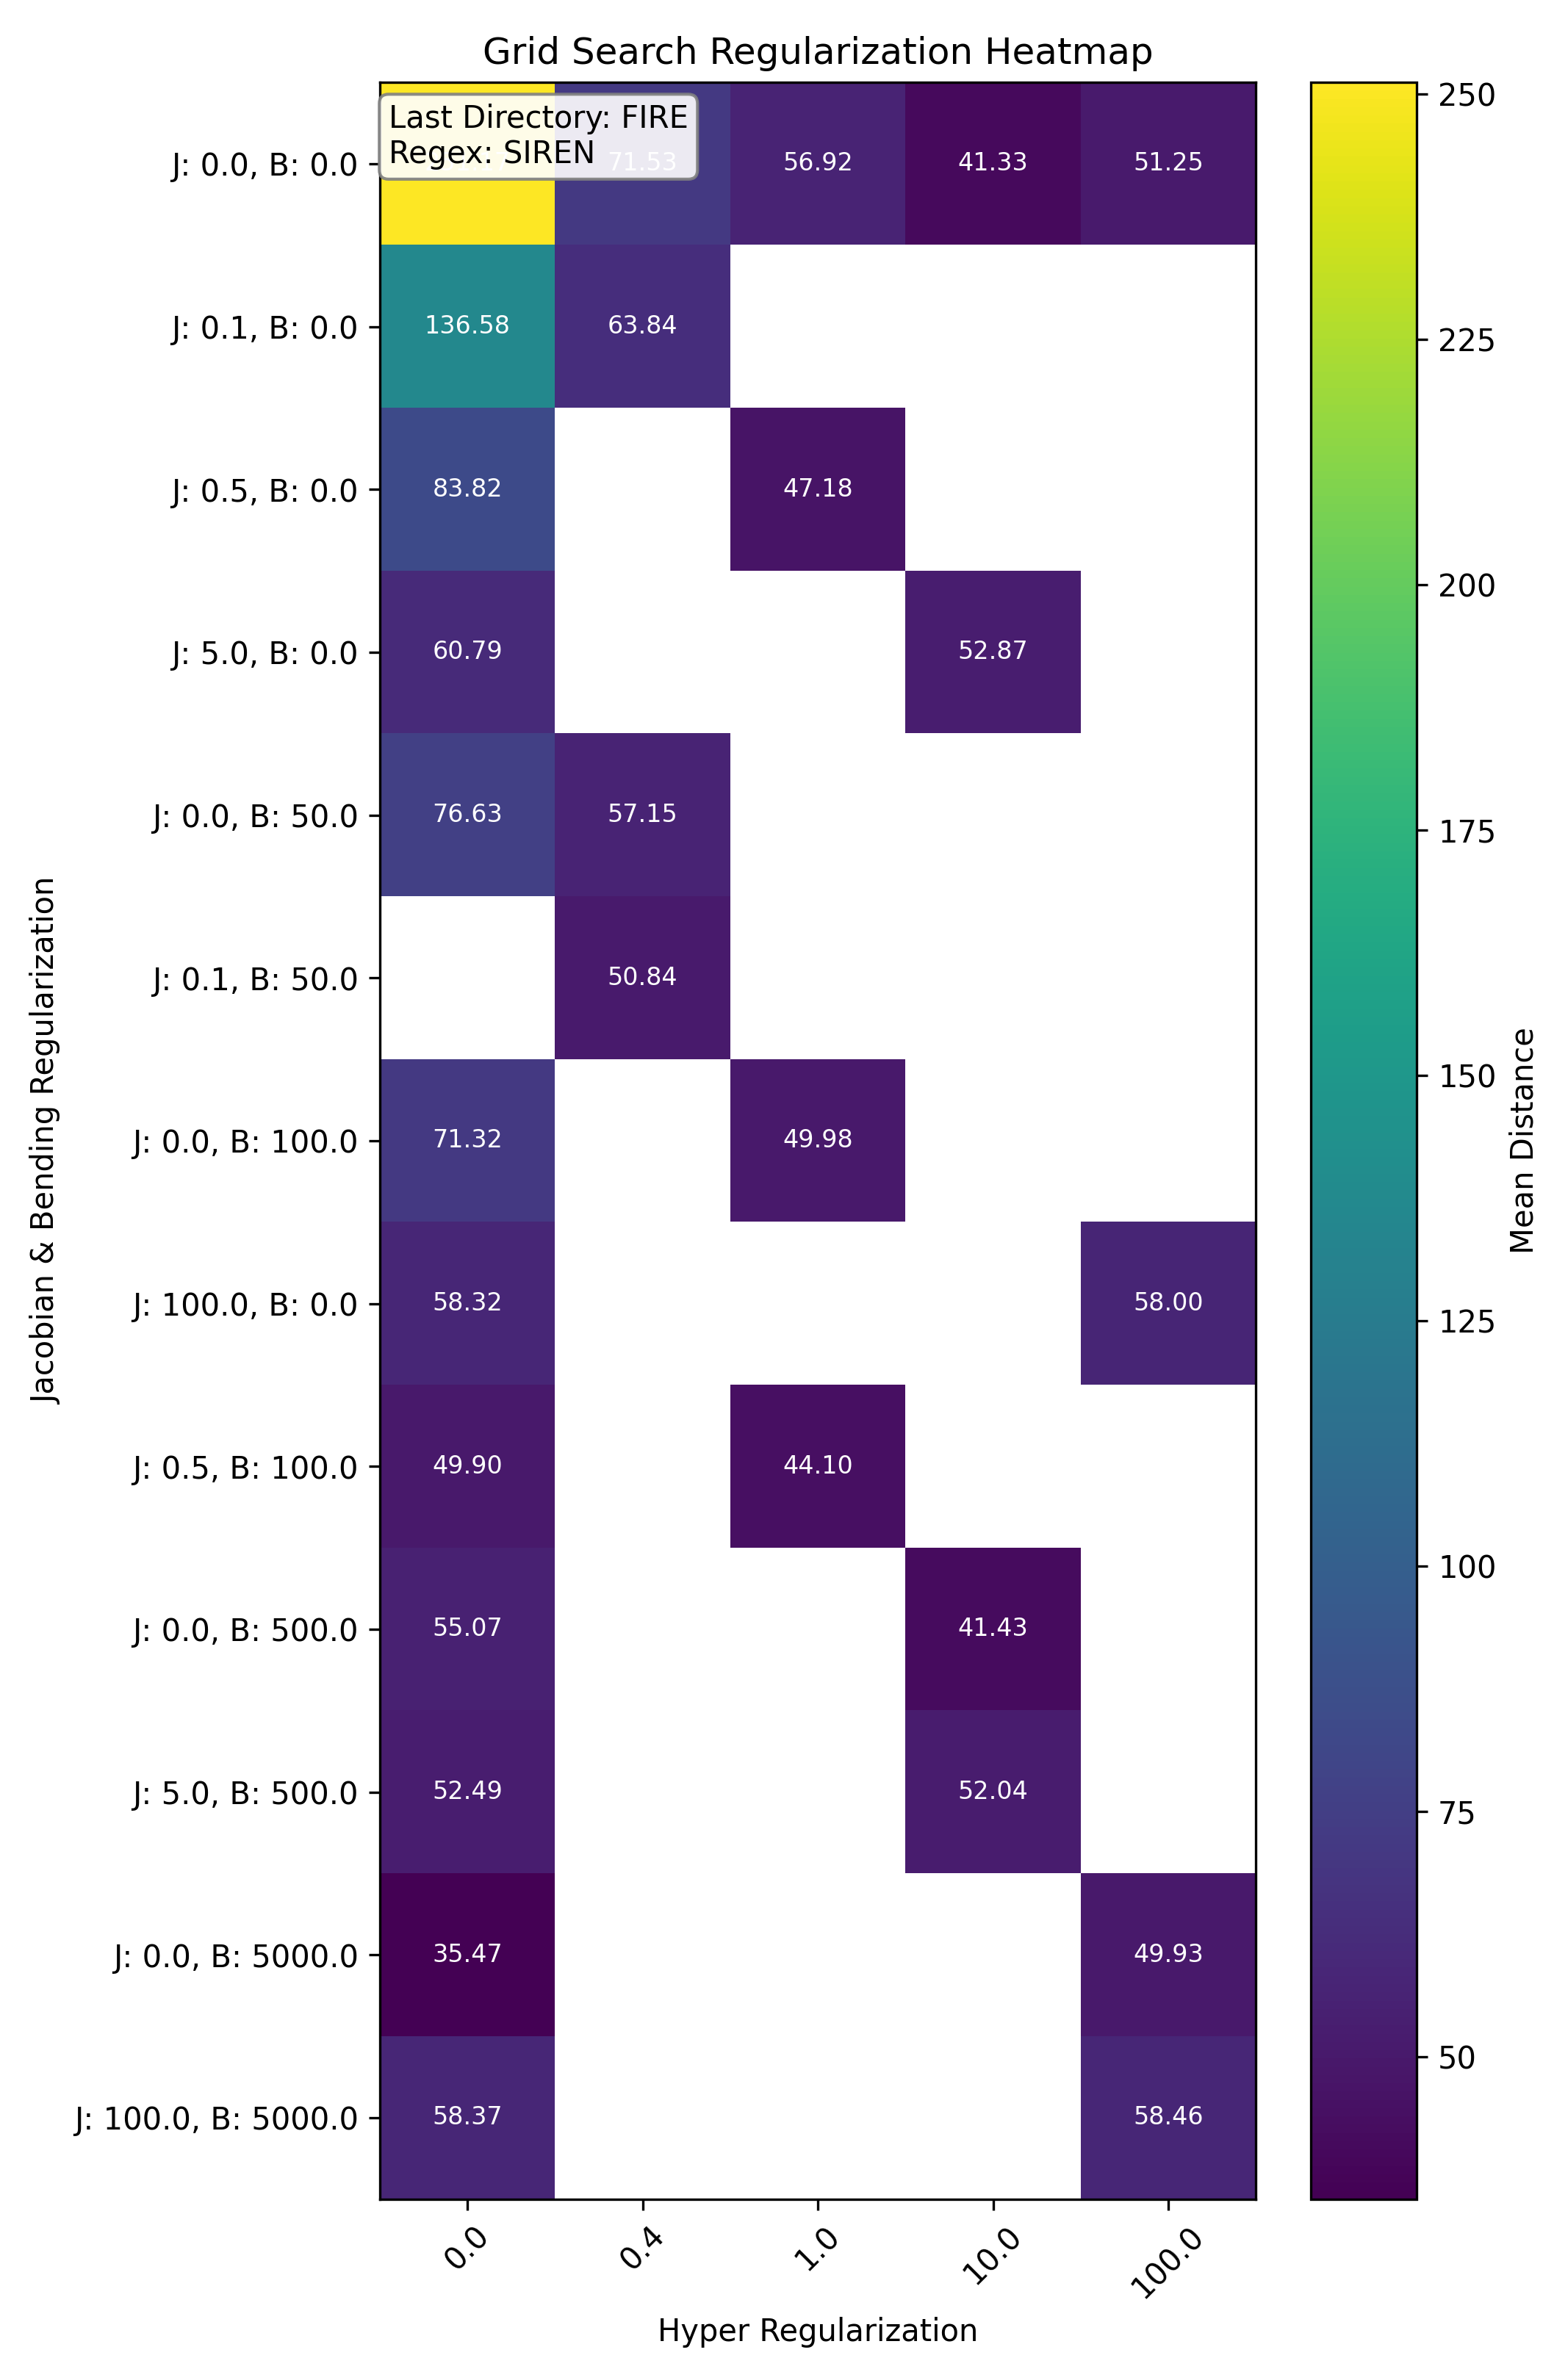
\includegraphics[width=\textwidth]{imaxes/grid_search_single_heatmap_FIRE_SIREN.png}
        \caption{FIRE - SIREN}
        \label{fig:gs_single_FIRE_SIREN}
    \end{subfigure}
    
    \vskip0\baselineskip
    
    \begin{subfigure}[b]{0.45\textwidth}
        \centering
        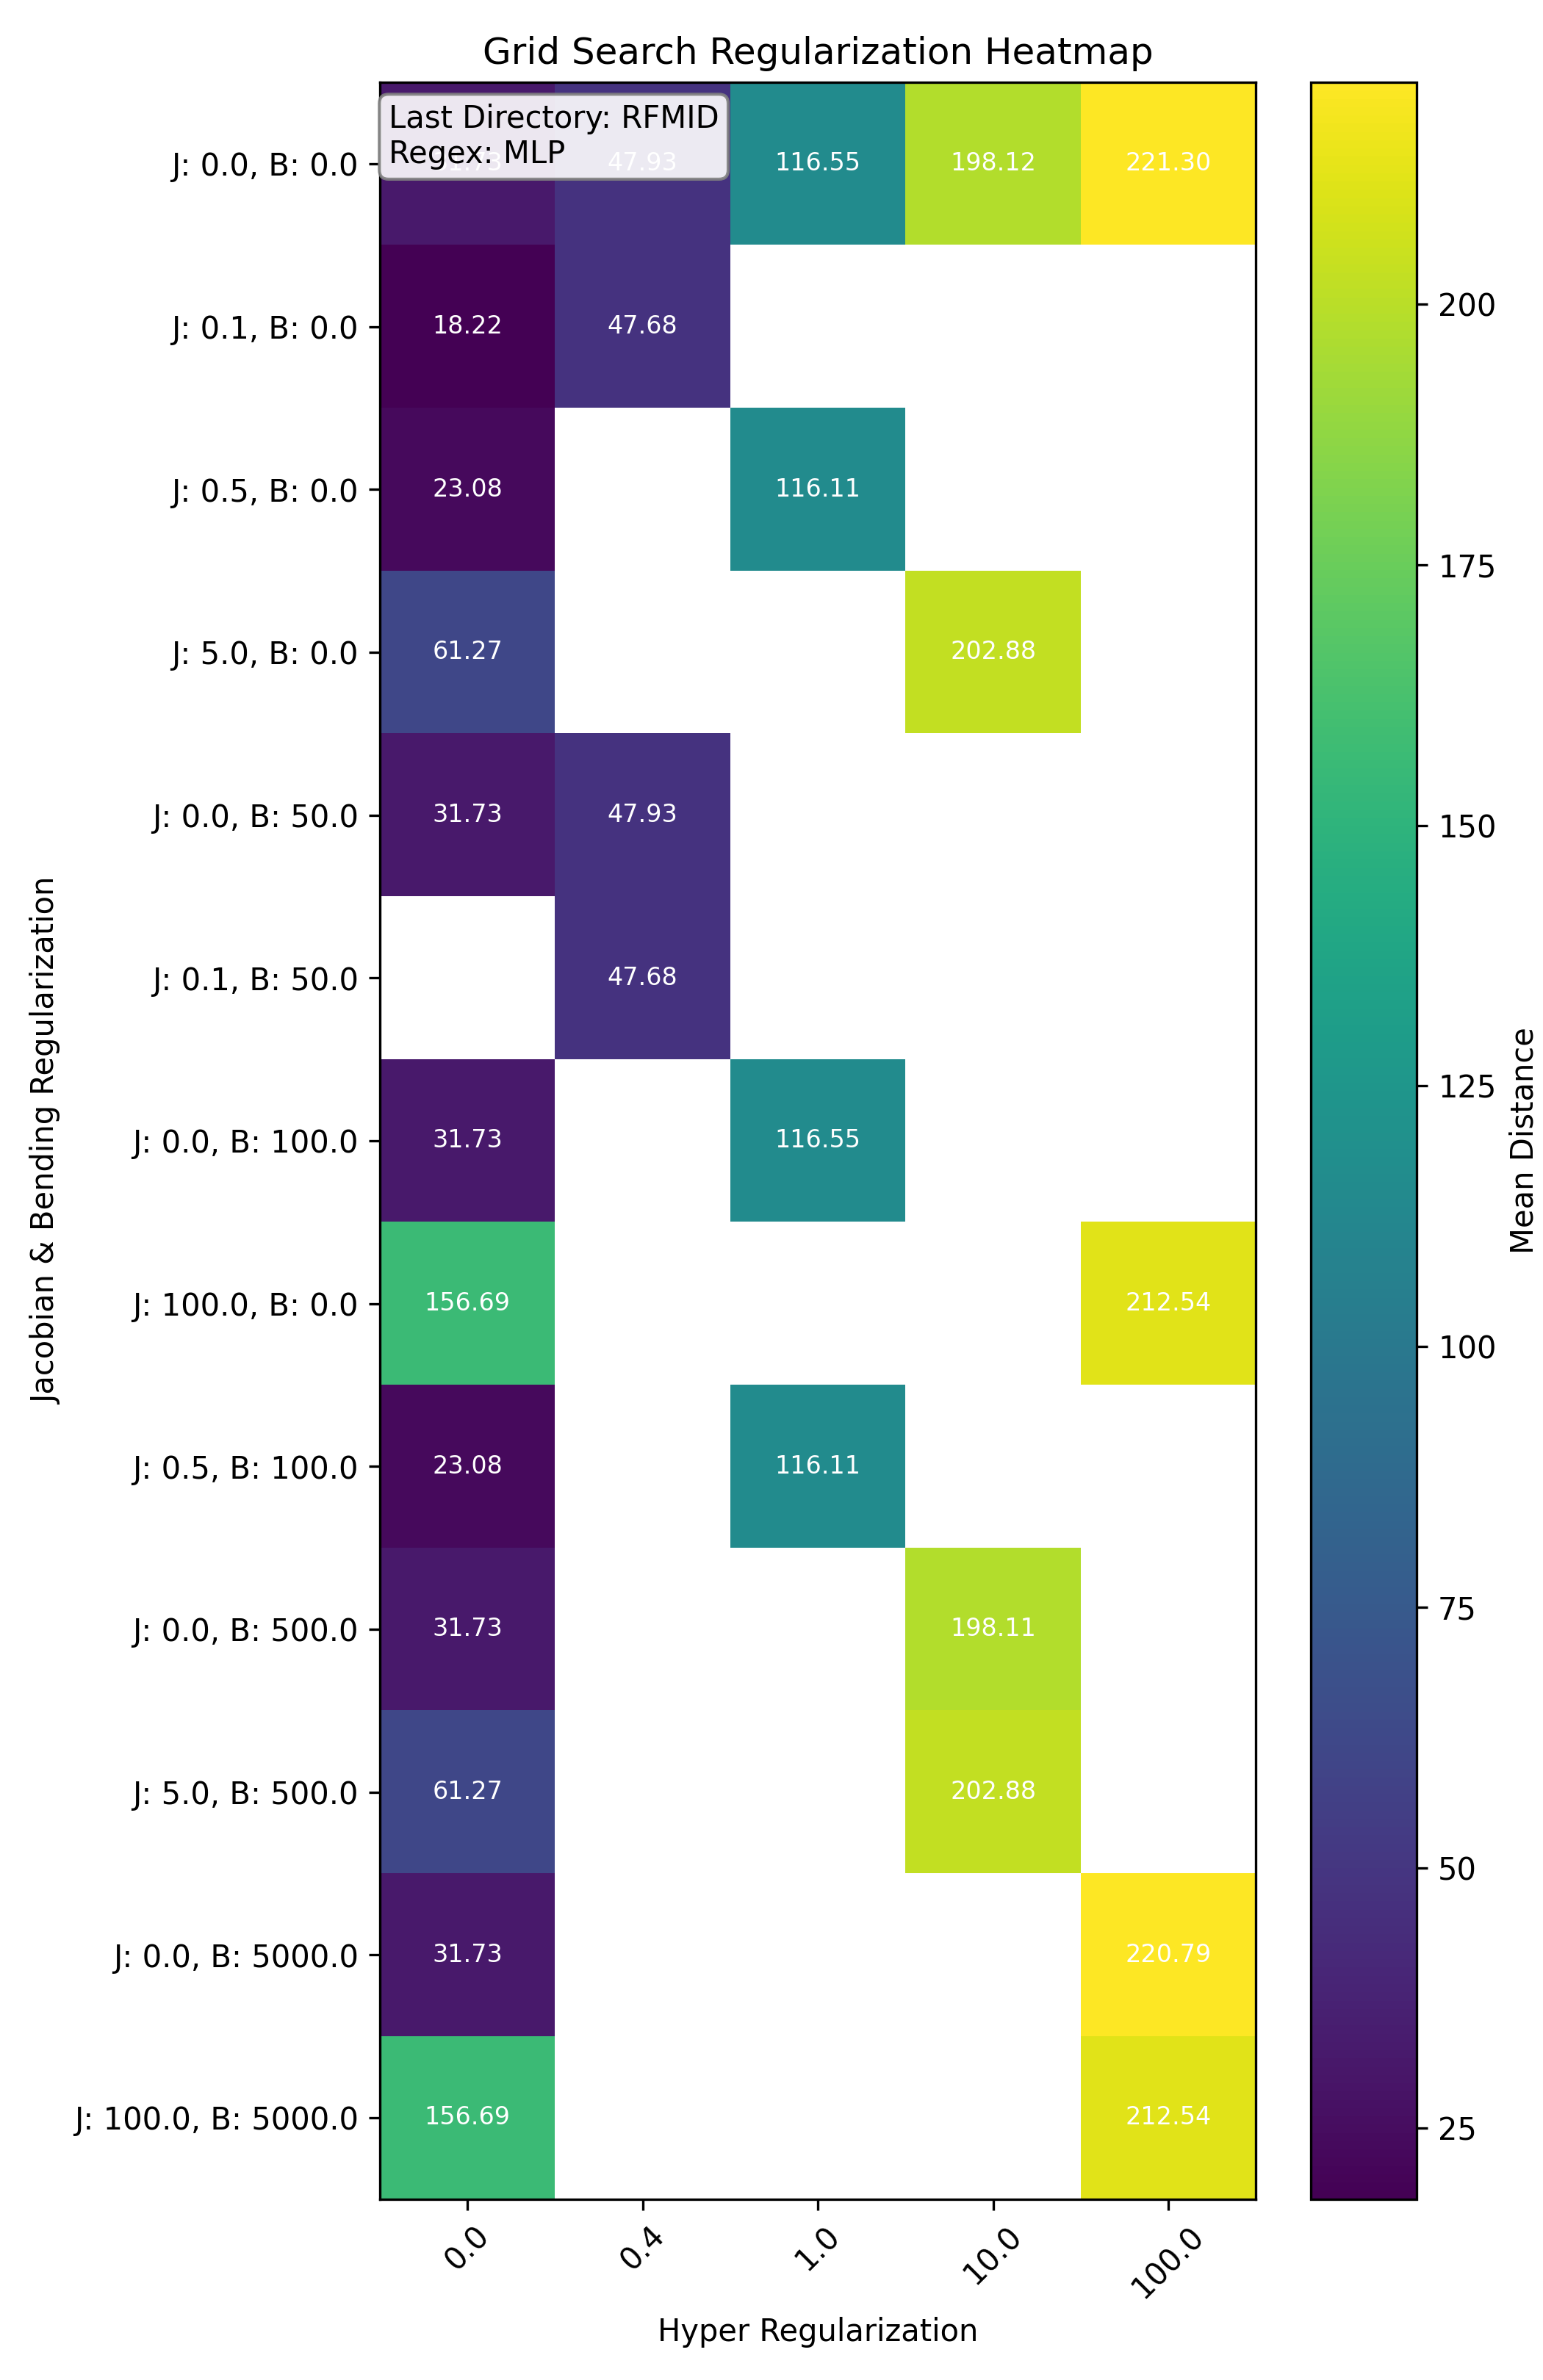
\includegraphics[width=\textwidth]{imaxes/grid_search_single_heatmap_RFMID_MLP.png}
        \caption{RFMID - Relu}
        \label{fig:gs_single_RFMID_MLP}
    \end{subfigure}\hfill
    \begin{subfigure}[b]{0.45\textwidth}
        \centering
        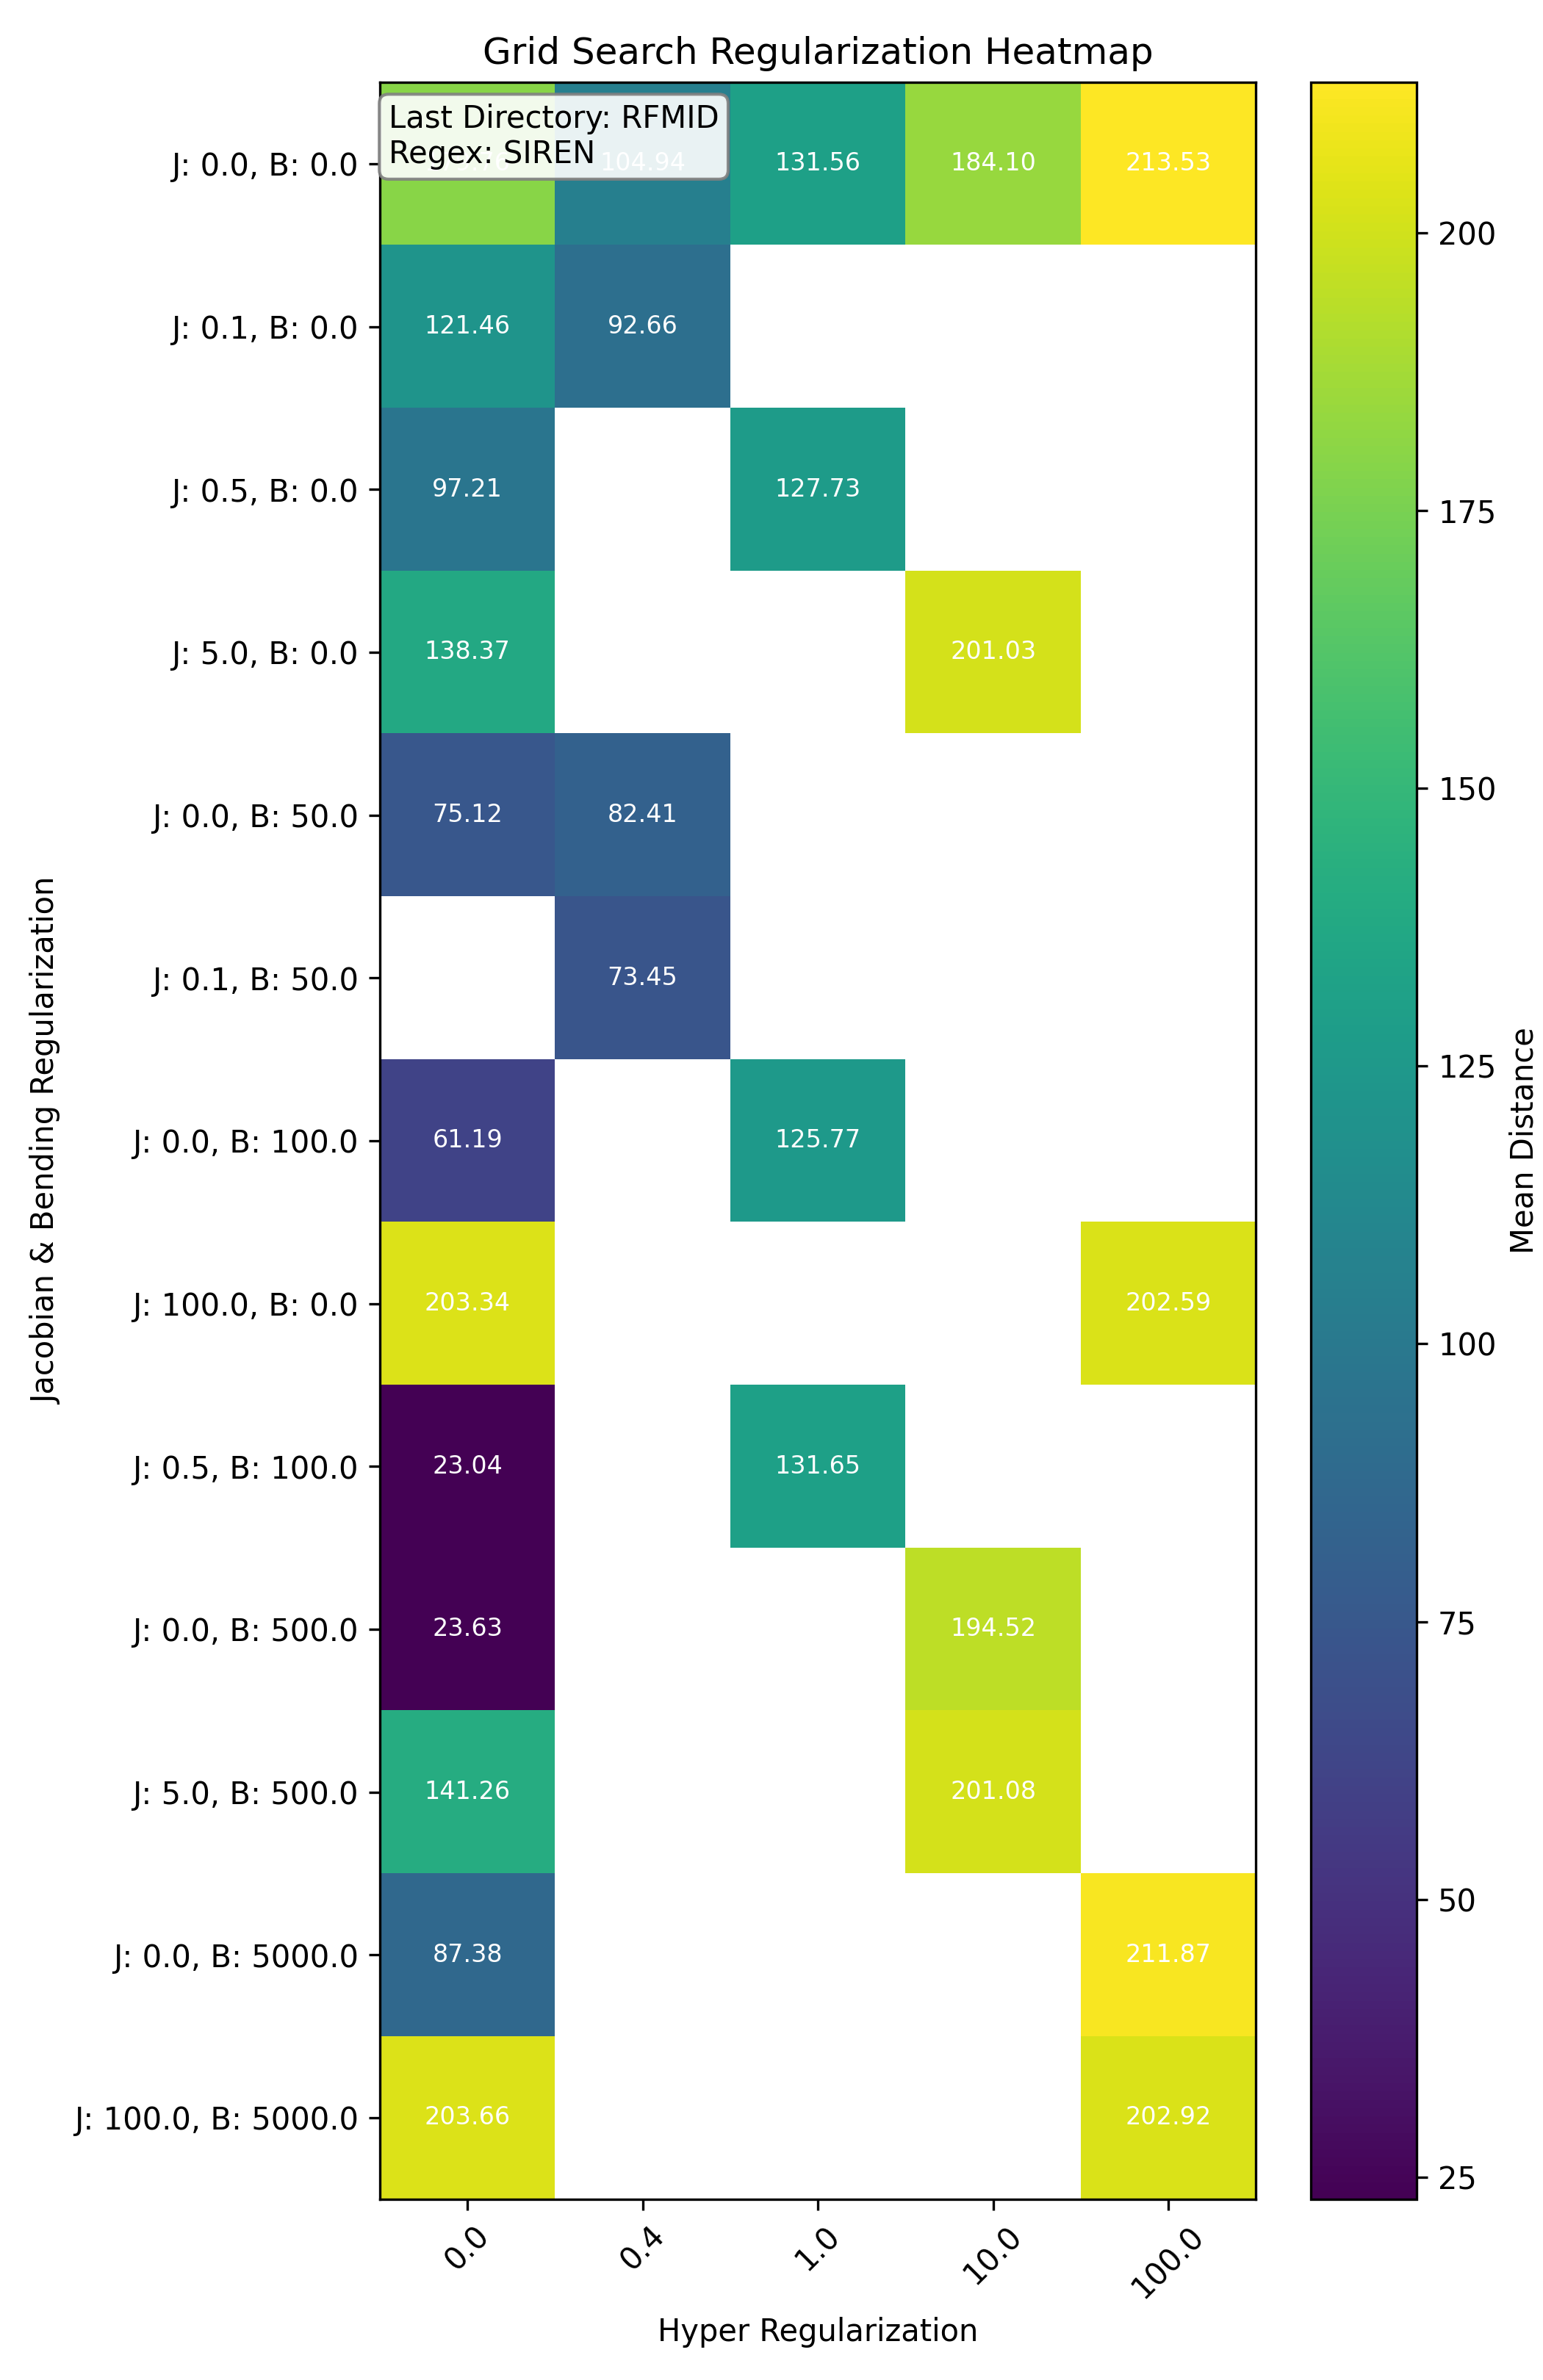
\includegraphics[width=\textwidth]{imaxes/grid_search_single_heatmap_RFMID_SIREN.png}
        \caption{RFMID - SIREN}
        \label{fig:gs_single_RFMID_SIREN}
    \end{subfigure}
    
    \caption{Mapa de calor cos resultados de diferentes combinacións de termos de regularización e funcións de activación sobre os datasets FIRE e RFMID}
    \label{fig:gs_single_heatmaps}
\end{figure}

\paragraph{Discusión}
\label{par:Discusion-regularization}

Os resultados amosan que a regularización ten un impacto significativo no rendemento da rede.

\paragraph{Conclusións}
\label{par:Conclusions-regularization}

\subsubsection{Learning rate}
\label{subsubsec:Learning rate}

\paragraph{Planteamento}
\label{par:Planteamento-learningrate}

O learning rate é un parámetro do optimizador (Adam neste caso) que regula o tamaño dos axustes efectuados aos parámetros do modelo durante cada iteración de actualización. Determina a magnitude do cambio aplicado para minimizar a función de perda, afectando tanto a velocidade de converxencia como a estabilidade do proceso de aprendizaxe.
Un learning rate demasiado alto pode provocar que a rede diverxa, mentres que un learning rate demasiado baixo pode resultar en converxencia lenta ou quedar atrapado en mínimos locais.

Debido á natureza da rede, o batch size utilzado ten unha relación directa co learning rate, polo que tentaremos determinar a relación óptima entre ambos.

Unha das heurísiticas mais comúns para relacionar o learning rate e o batch size é a regla de escalado linear \cite{goyal2018accuratelargeminibatchsgd}. 
A regla indica que o learning rate óptimo debe escalarse linearmente co tamaño do batch size. 

Unha forma de explicar isto é, xa que con batches mais grandes temos unha mellor aproximación do gradiente real, é posible utilizar un learning rate maior sen que a rede diverxa.

Para determinar cal é o learning rate óptimo, realizáronse experimentos comparando o rendemento de cada un sobre unha mostra de imaxes dos datases de FIRE e RFMID cas diferentes funcións de activación.

\paragraph{Resultados}
\label{par:Resultados-learningrate}

\ref{fig:grid_search_lr}, \ref{fig:e_heatmap_MLP_RFMID}

\begin{figure}[ht]
    \centering
    \begin{subfigure}[b]{0.45\textwidth}
        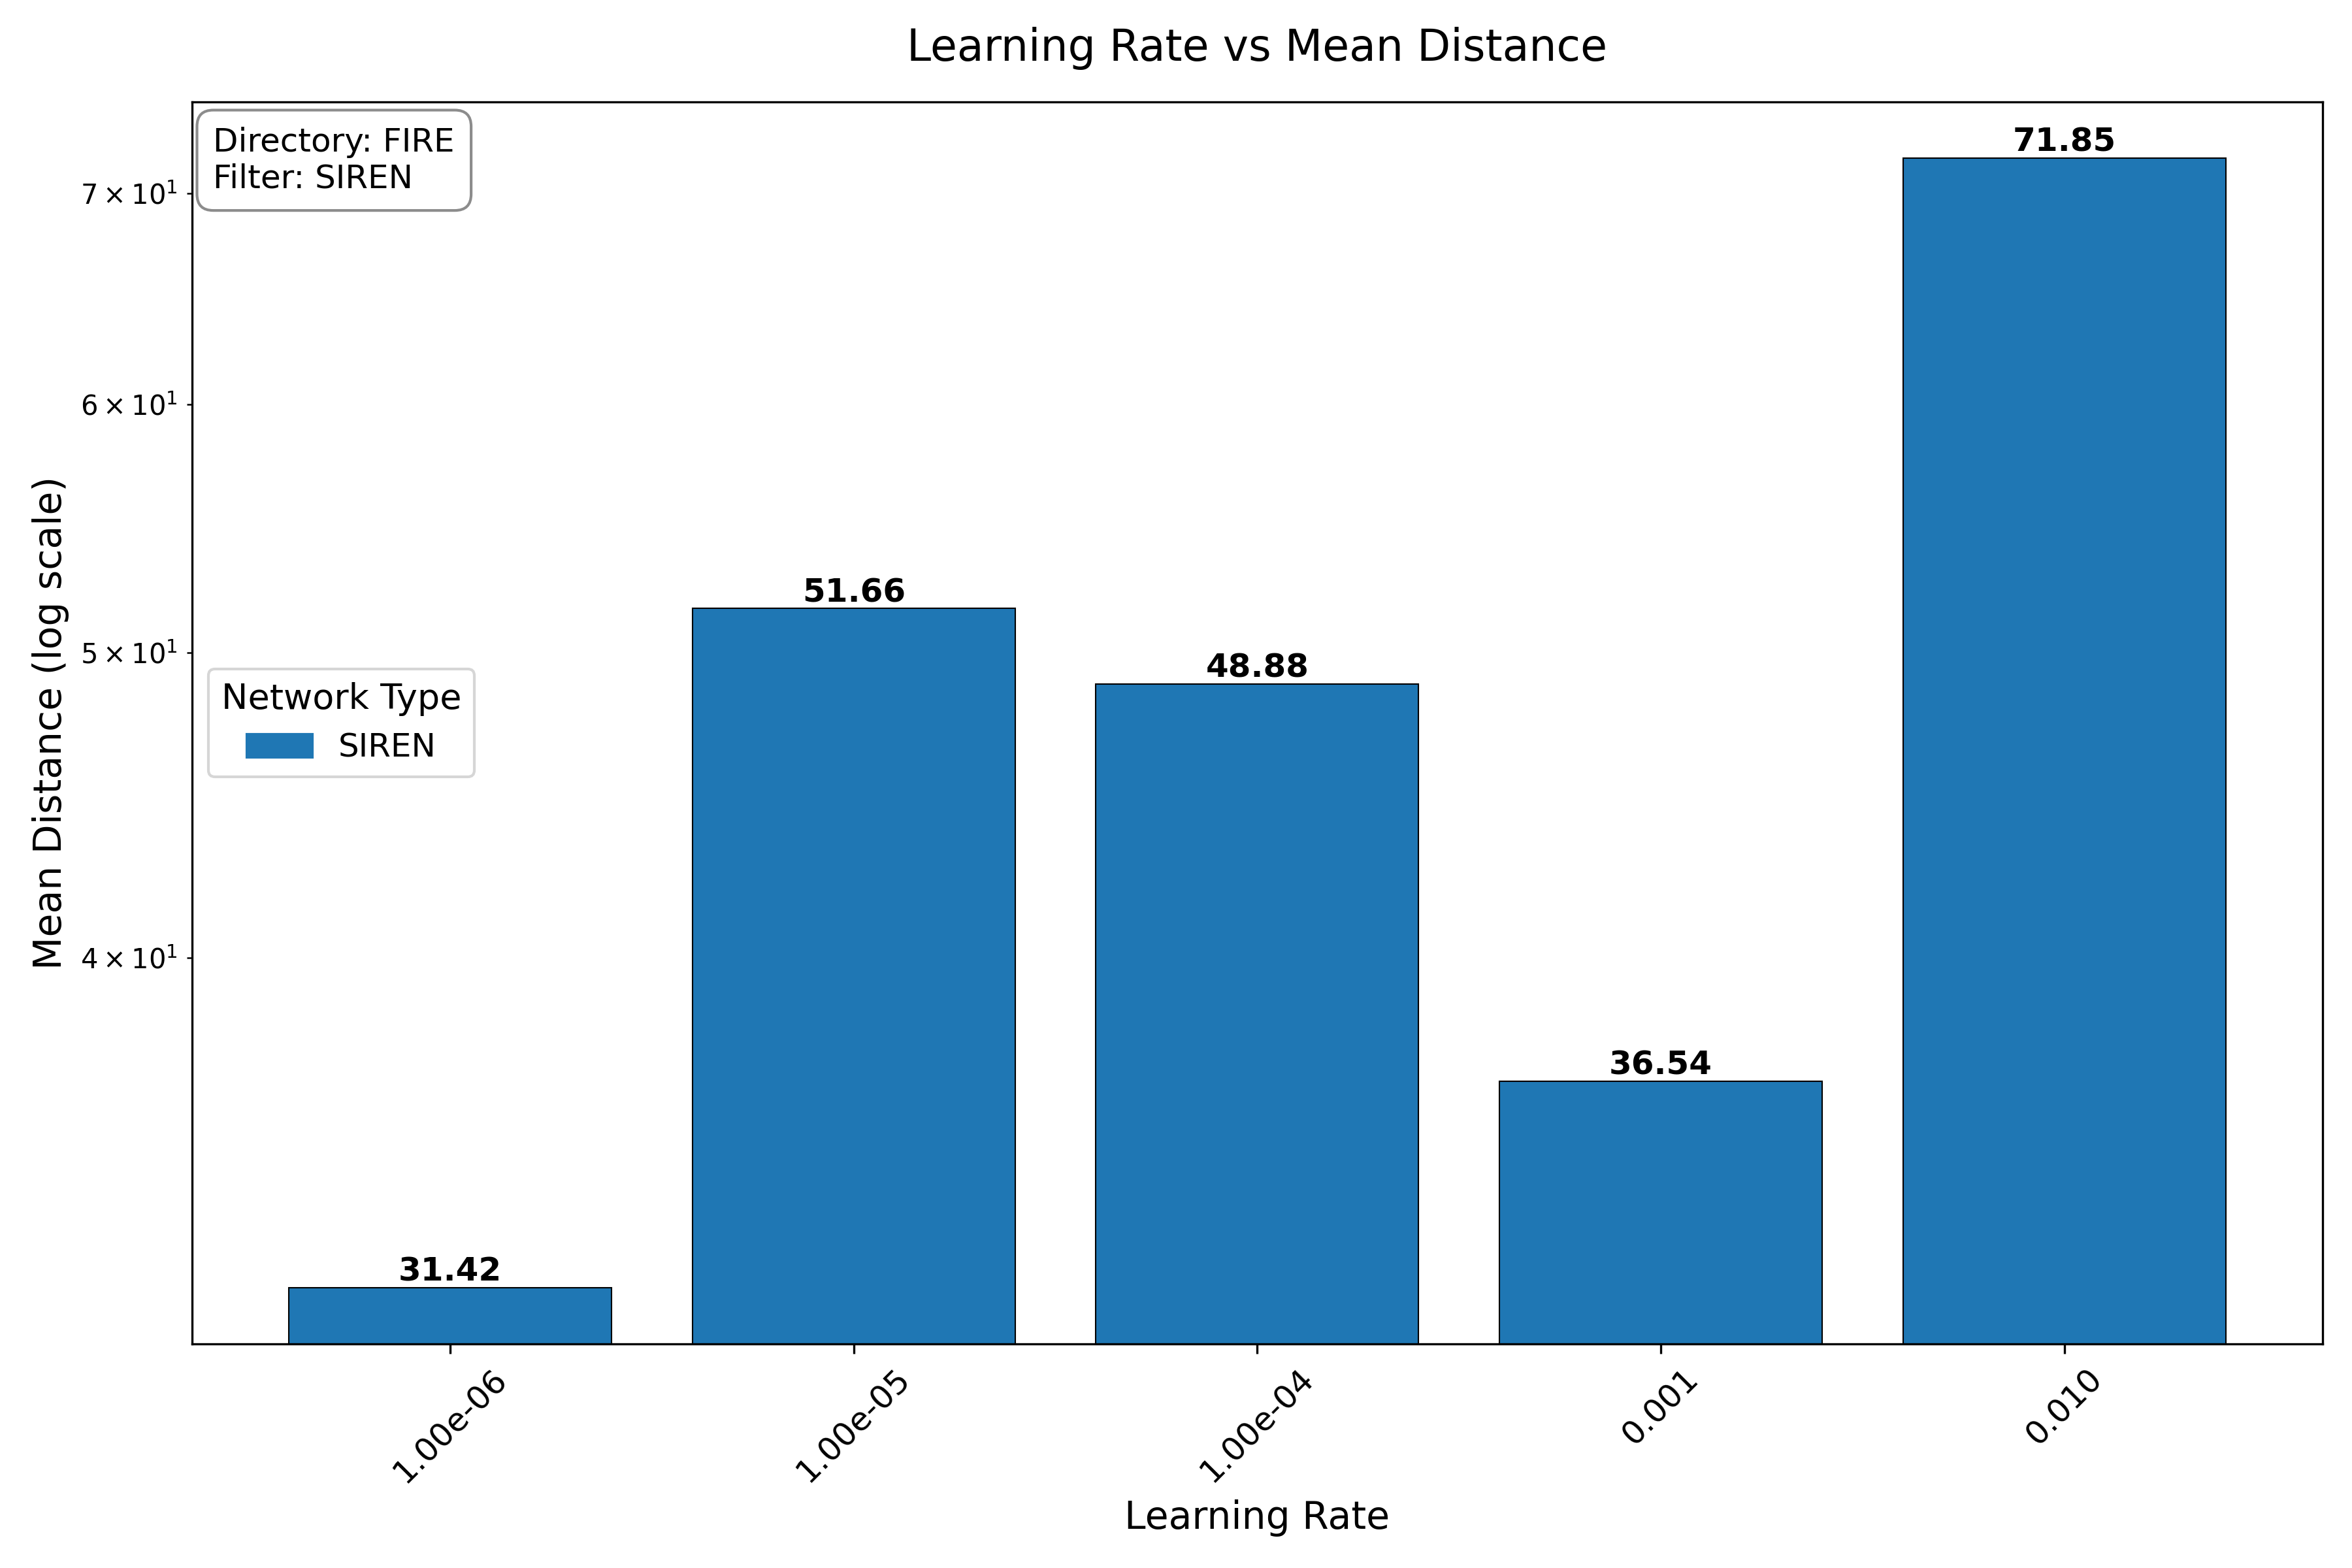
\includegraphics[width=\textwidth]{imaxes/grid_search_lr_FIRE_SIREN.png}
        \caption{FIRE - SIREN}
        \label{fig:grid_search_lr_FIRE_SIREN}
    \end{subfigure}\hfill
    \begin{subfigure}[b]{0.45\textwidth}
        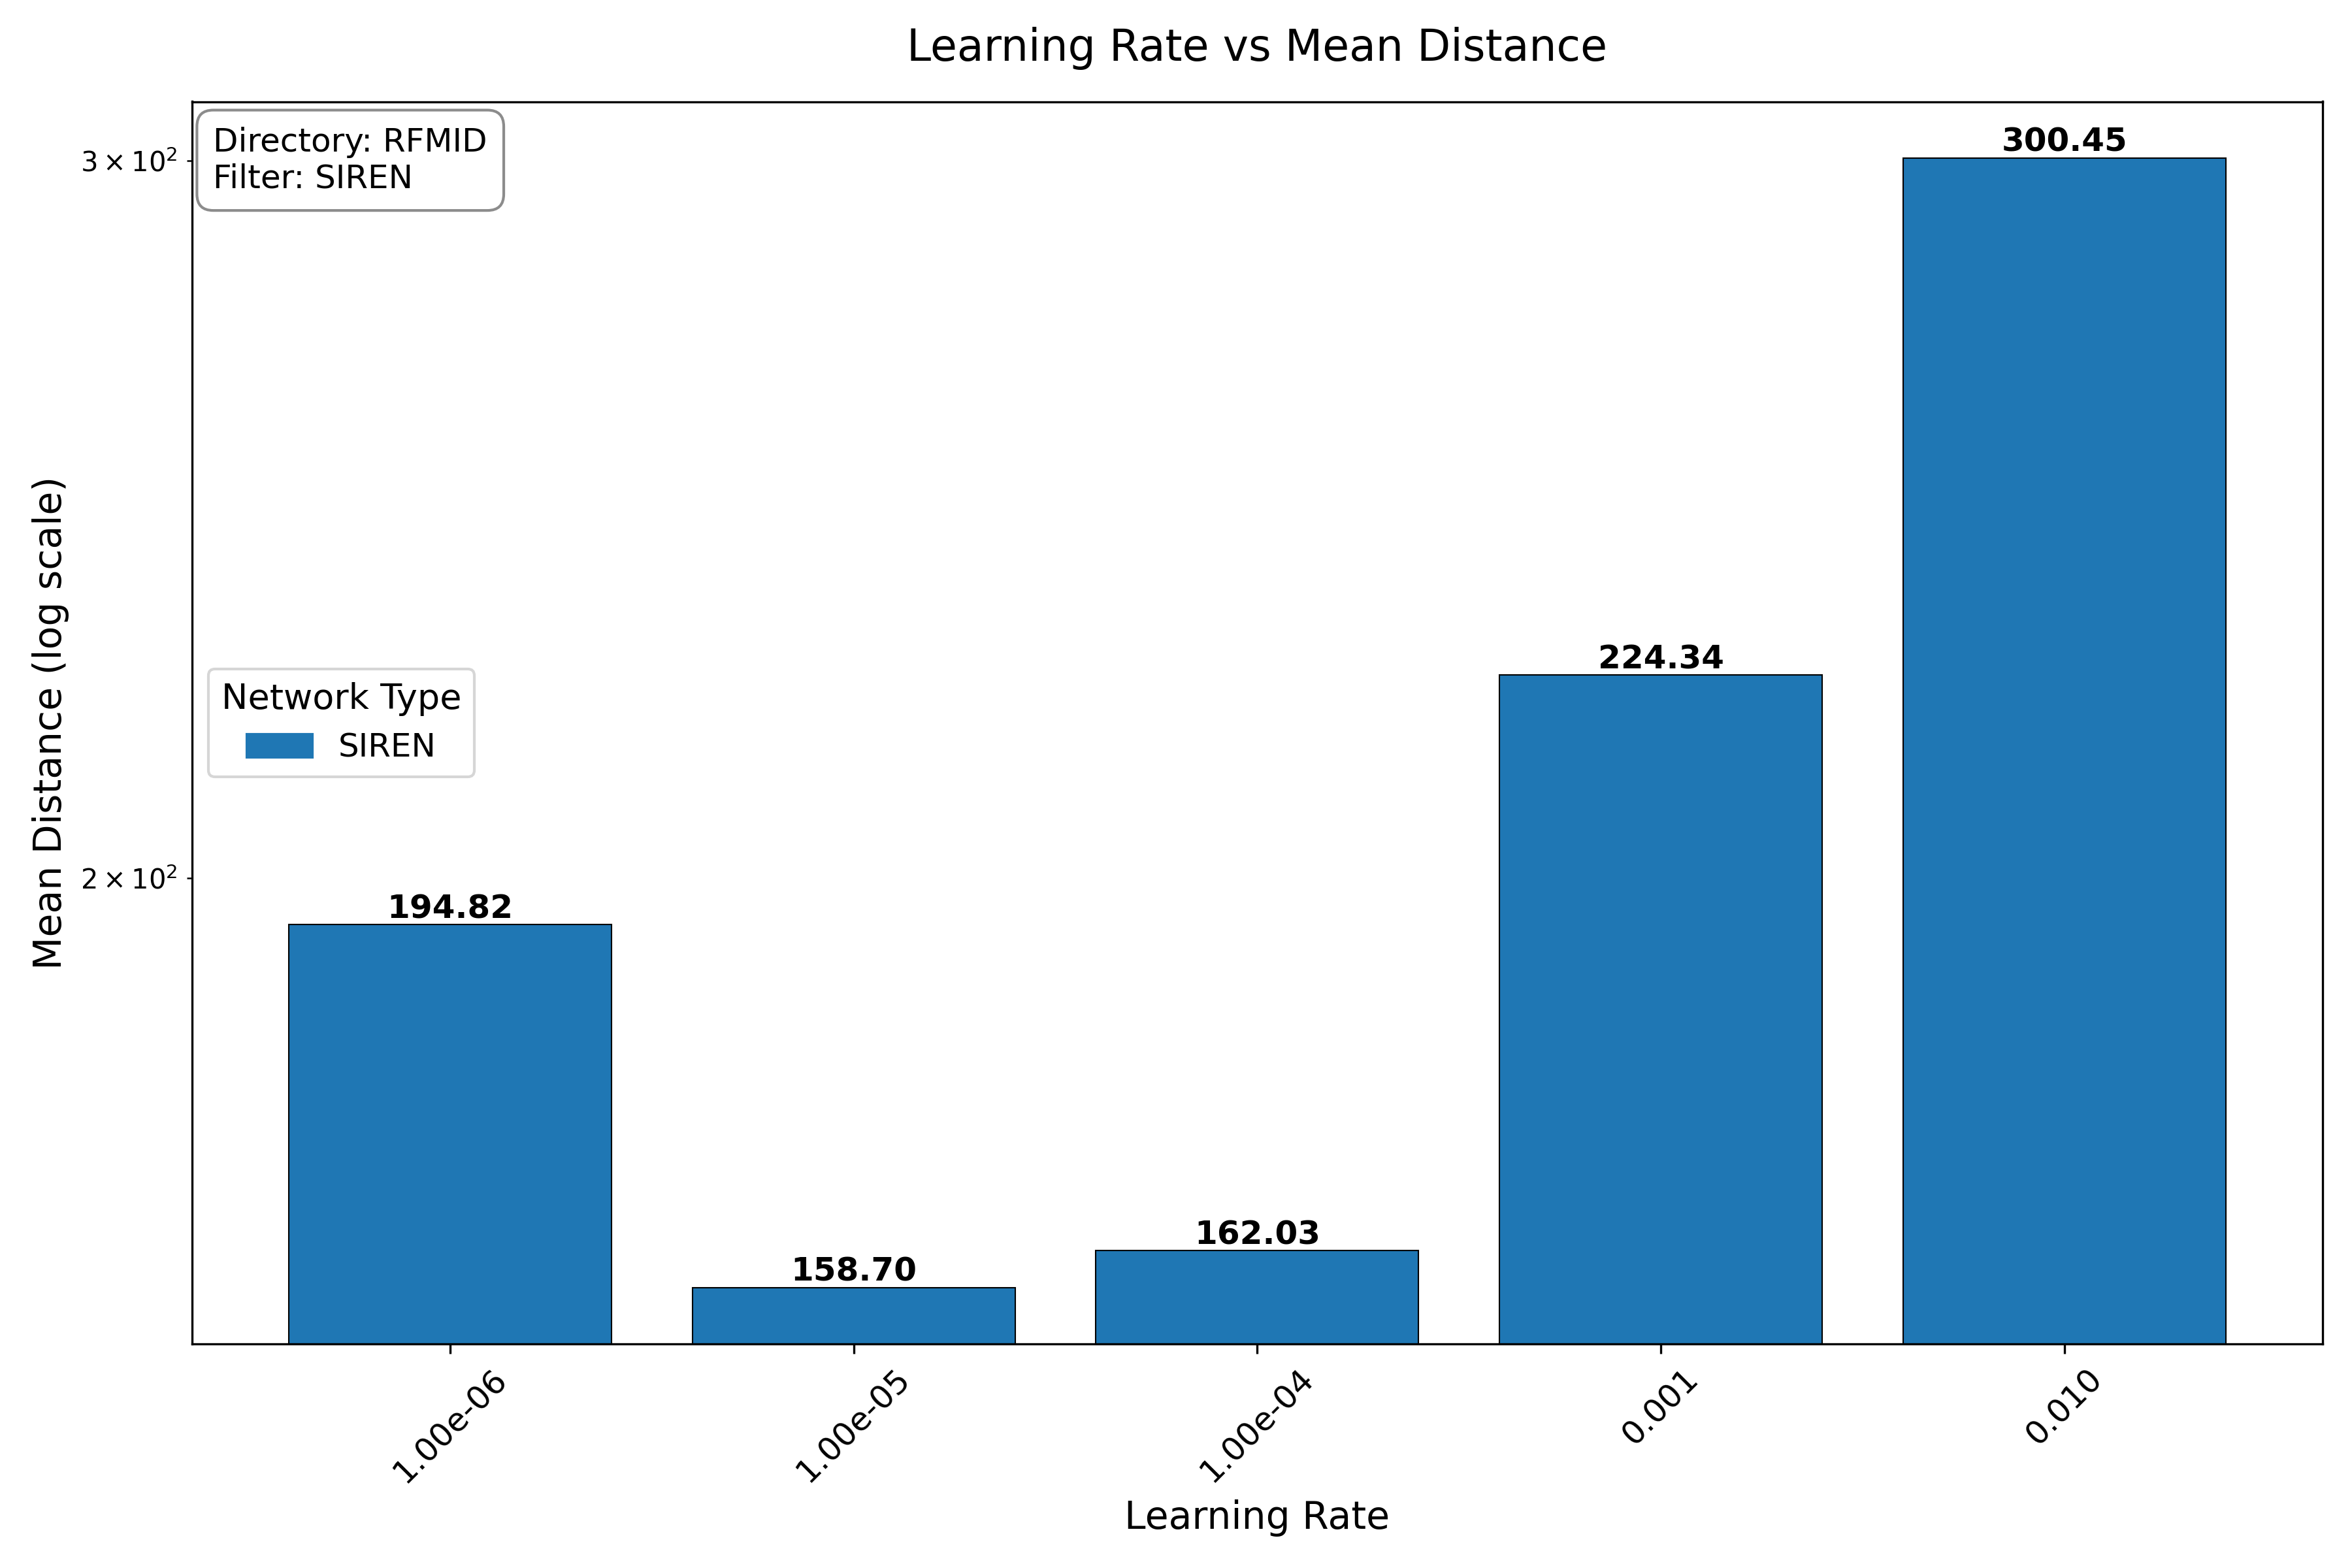
\includegraphics[width=\textwidth]{imaxes/grid_search_lr_RFMID_SIREN.png}
        \caption{RFMID - SIREN}
        \label{fig:grid_search_lr_RFMID_SIREN}
    \end{subfigure}
    \vskip\baselineskip
    \begin{subfigure}[b]{0.45\textwidth}
        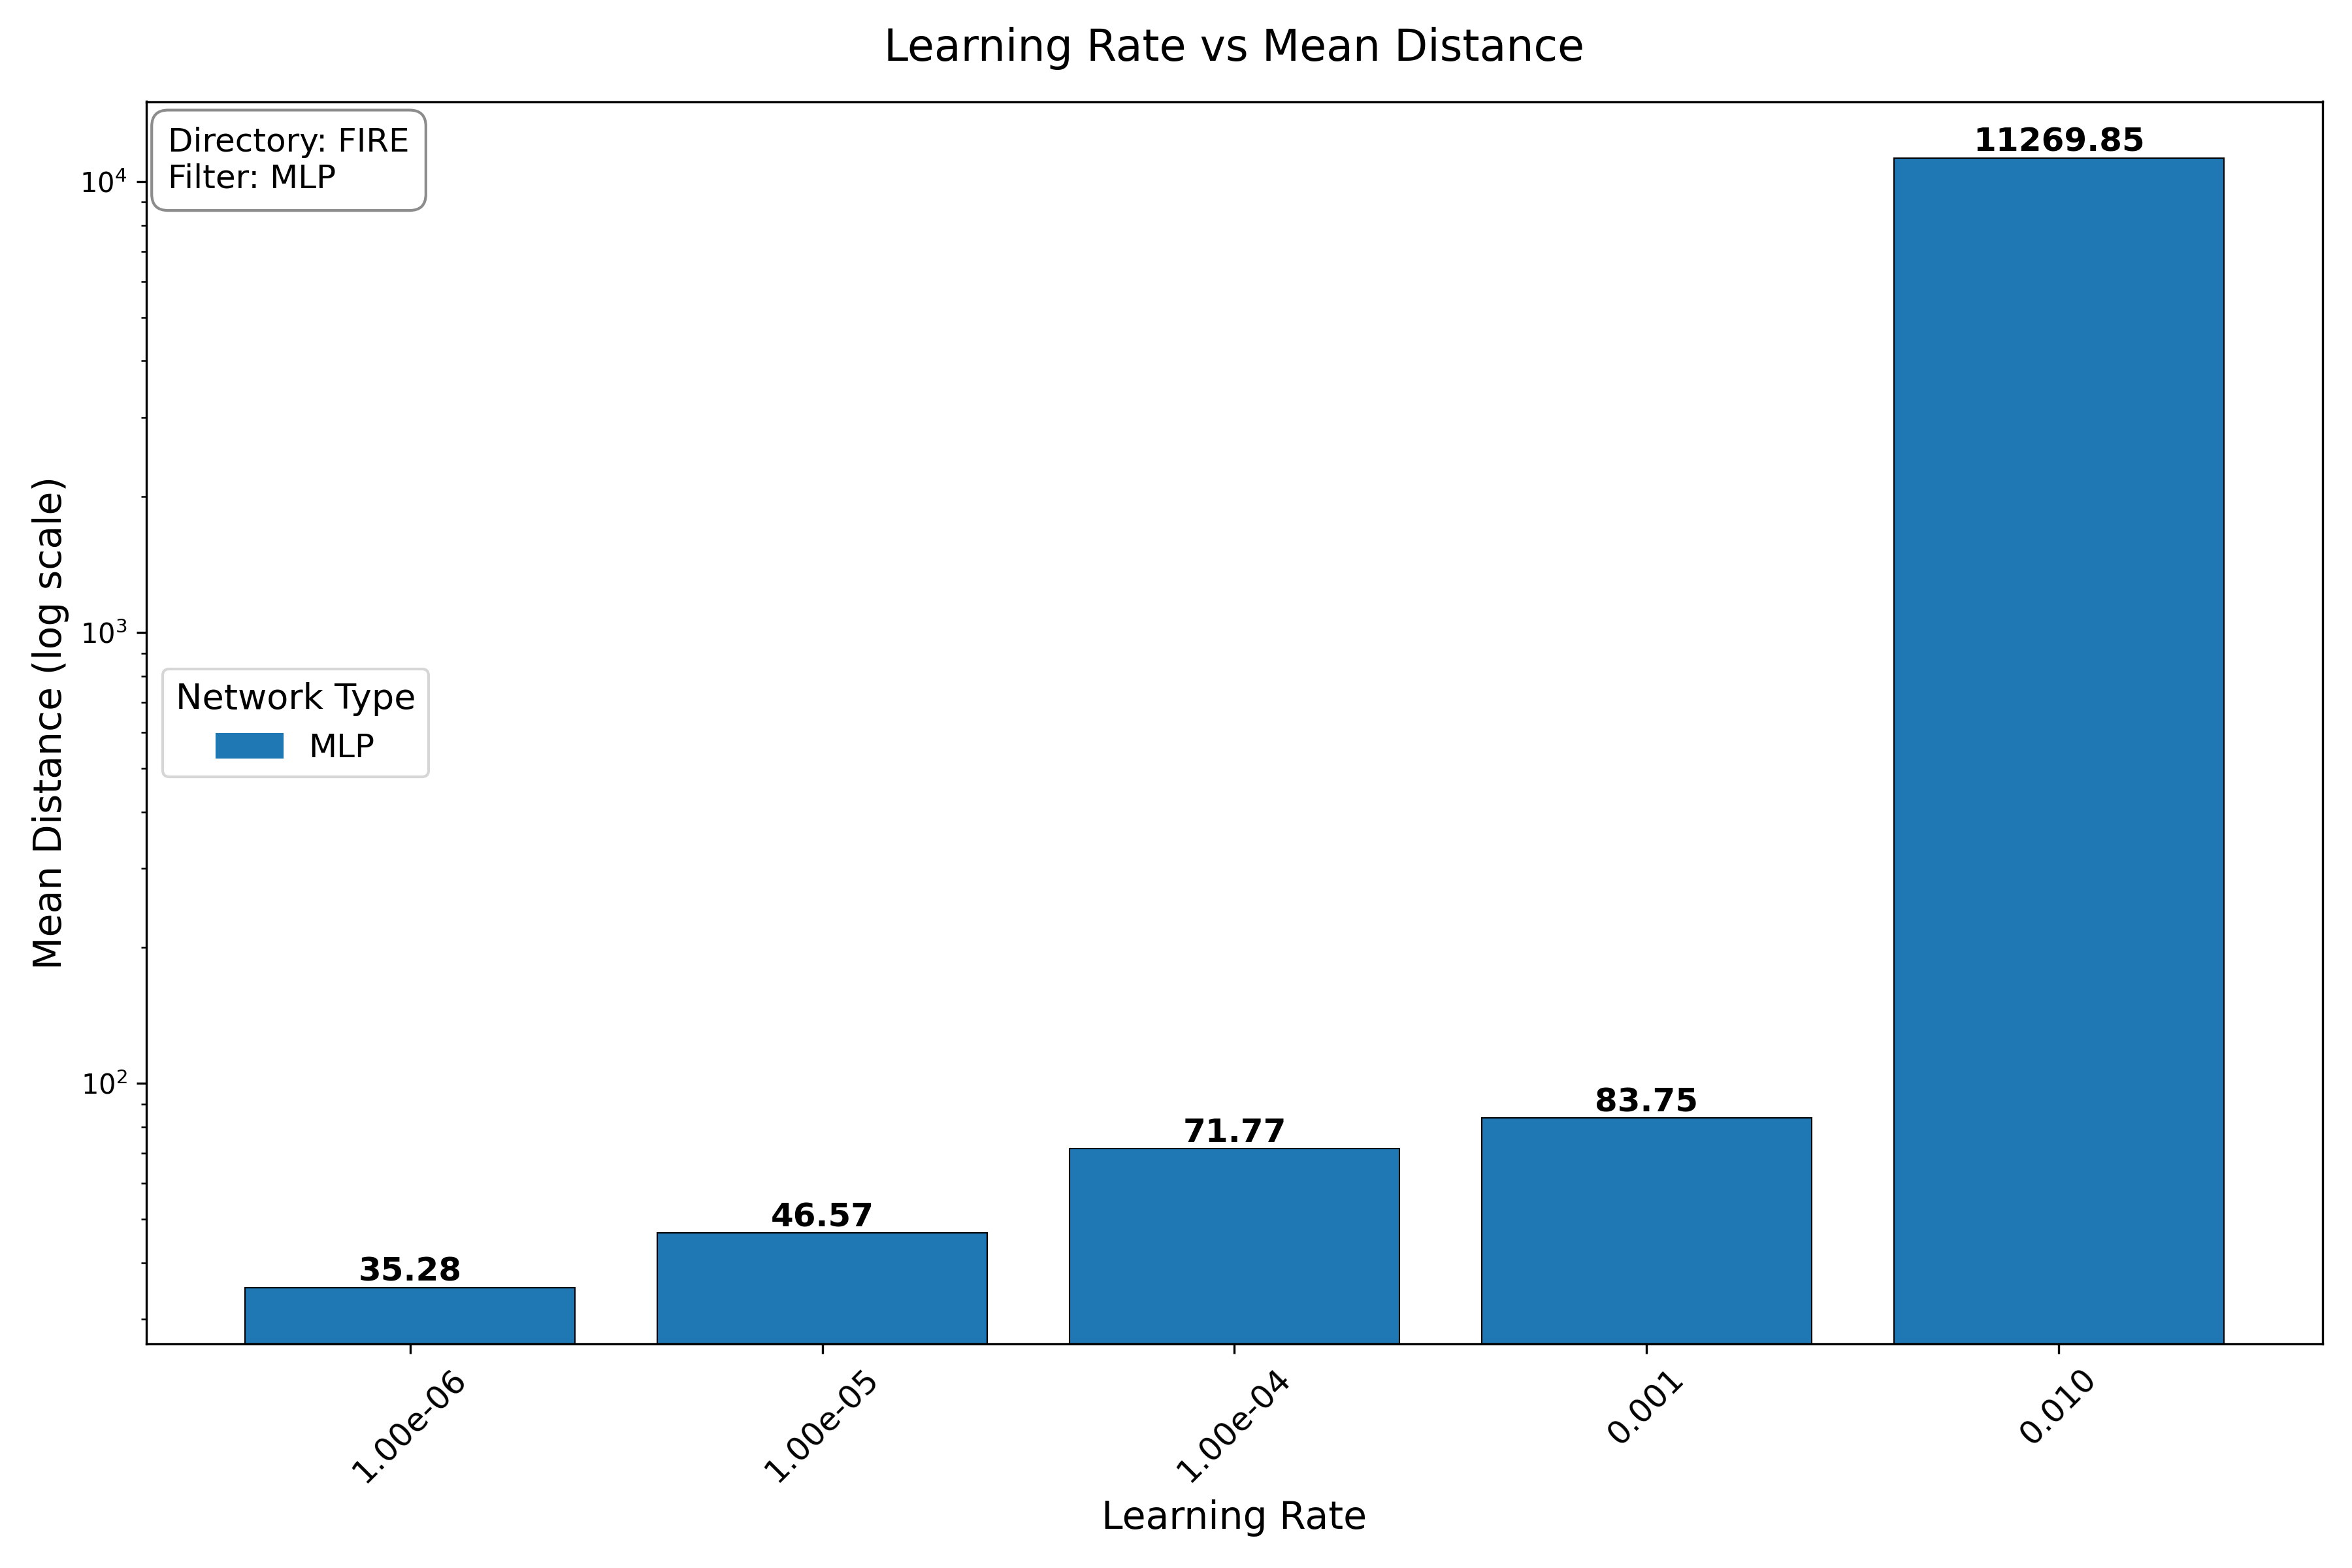
\includegraphics[width=\textwidth]{imaxes/grid_search_lr_FIRE_MLP.png}
        \caption{FIRE - Relu}
        \label{fig:grid_search_lr_FIRE_MLP}
    \end{subfigure}\hfill
    \begin{subfigure}[b]{0.45\textwidth}
        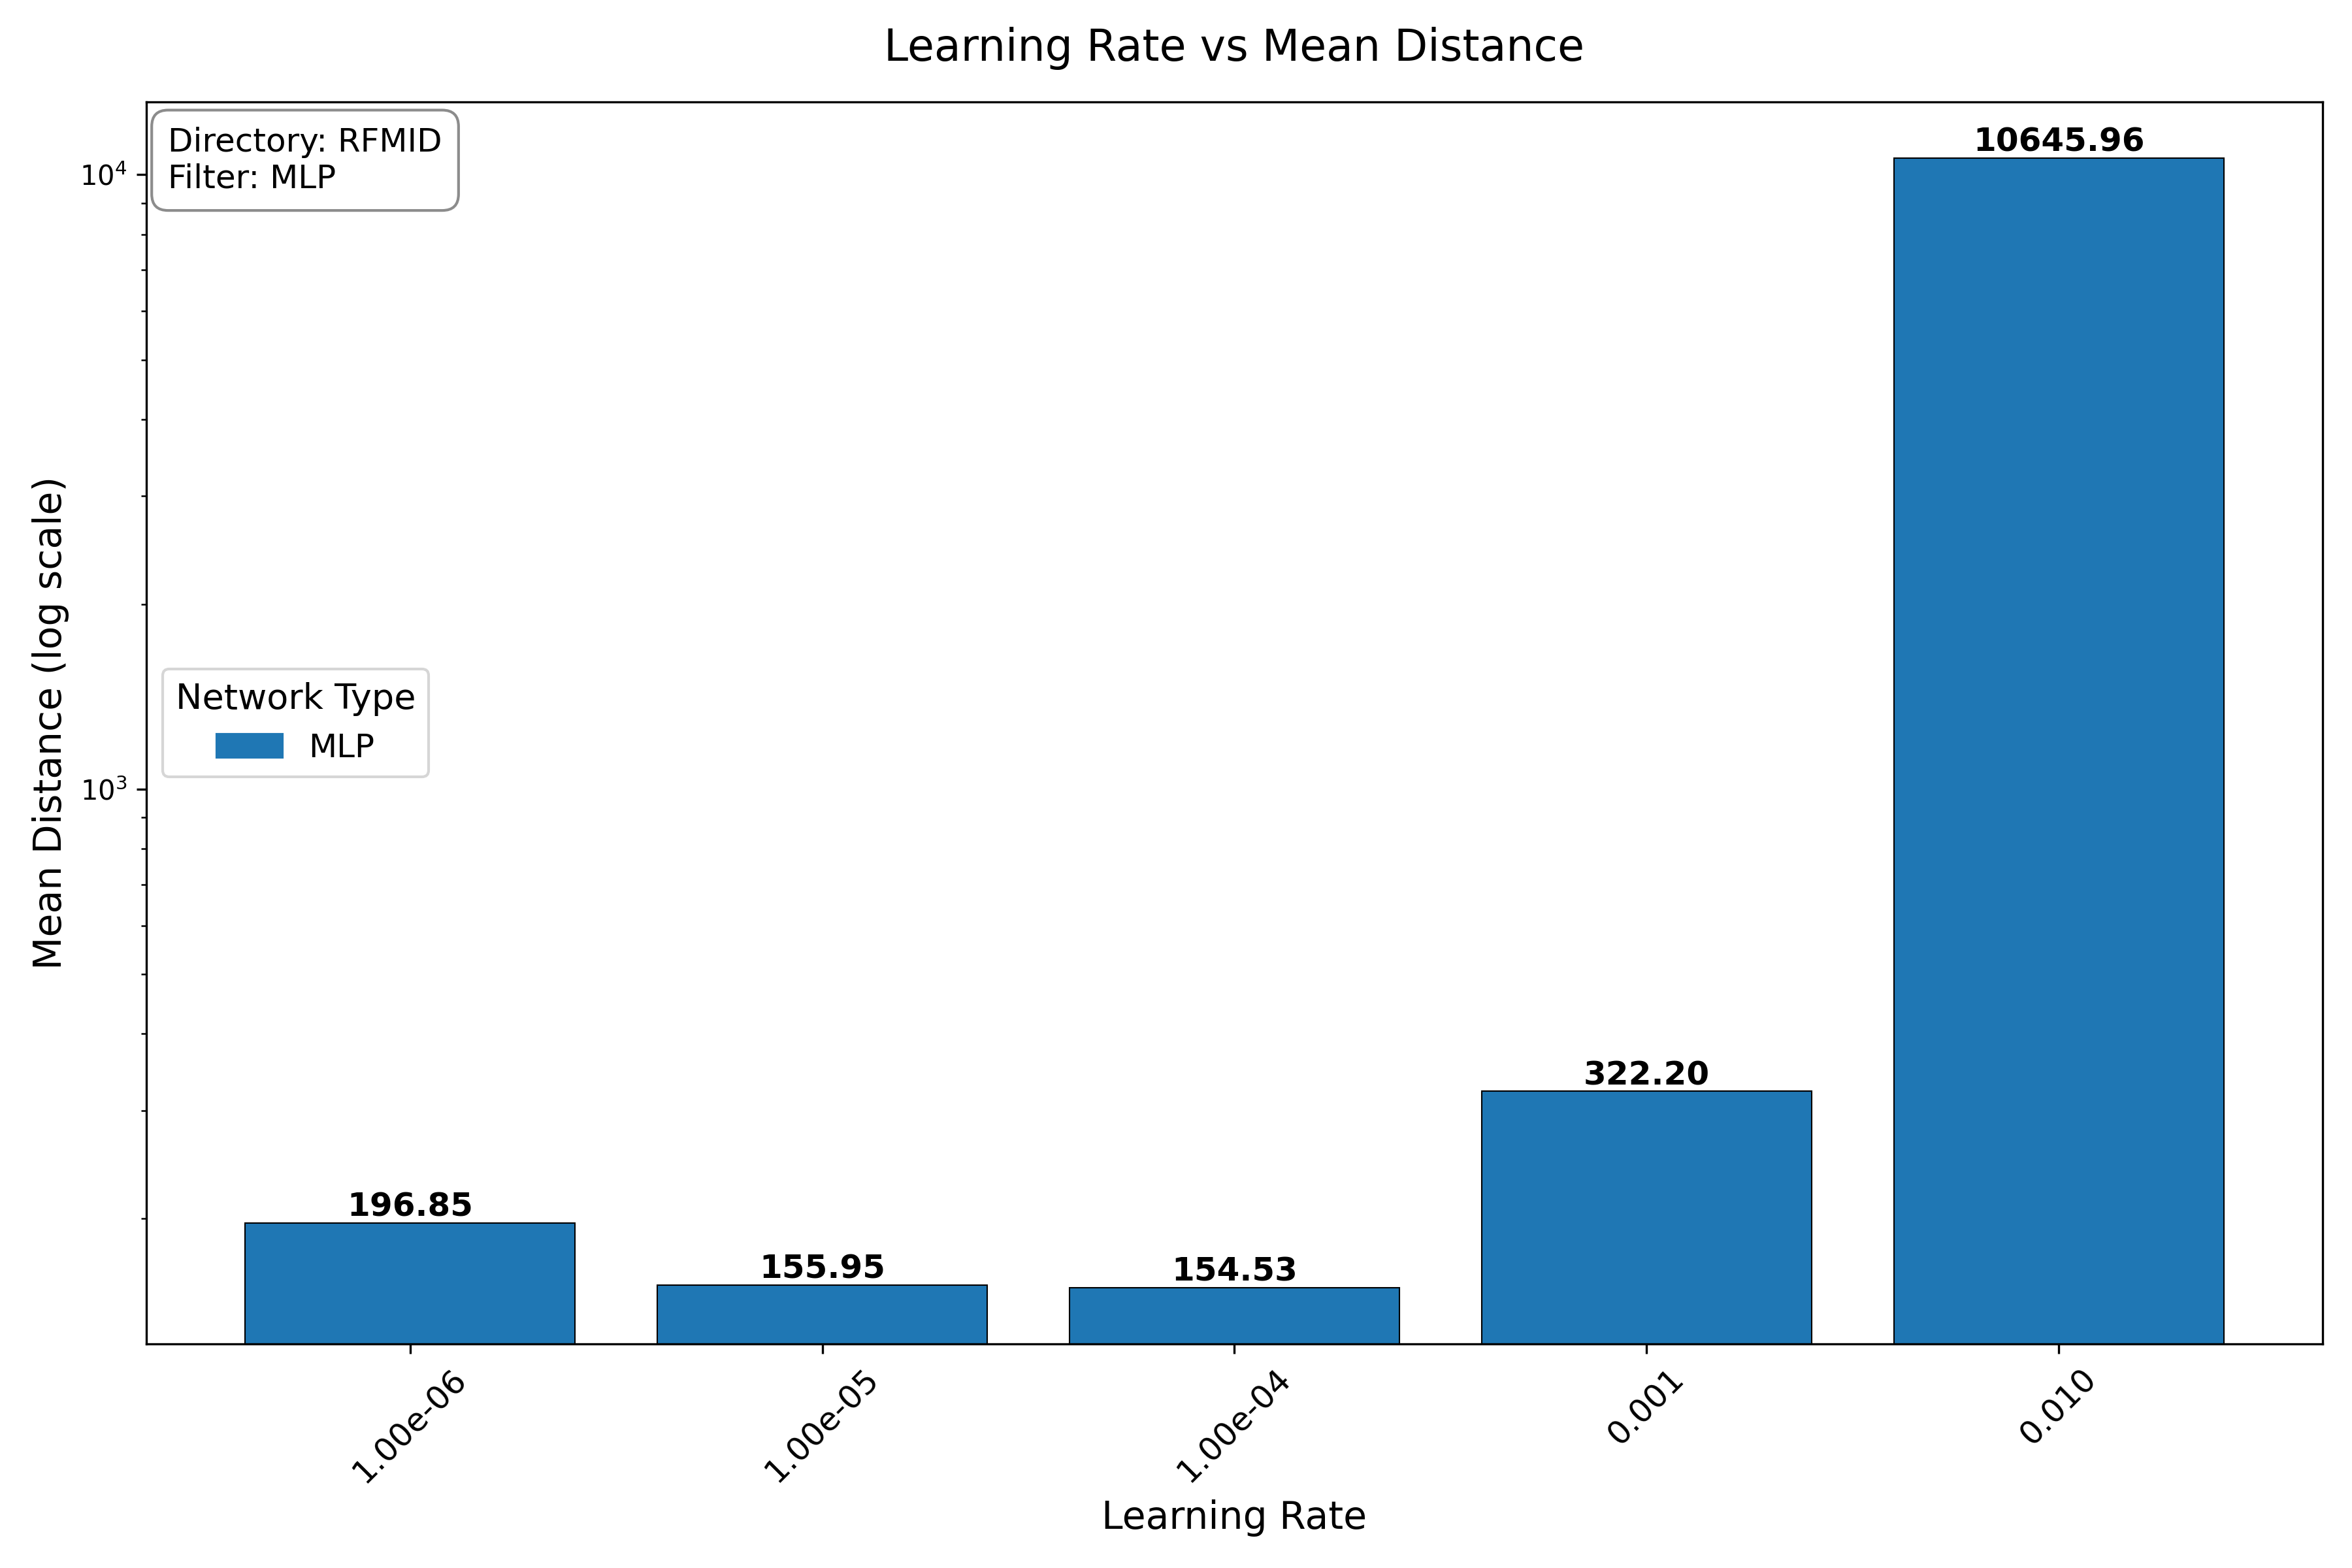
\includegraphics[width=\textwidth]{imaxes/grid_search_lr_RFMID_MLP.png}
        \caption{RFMID - Relu}
        \label{fig:grid_search_lr_RFMID_MLP}
    \end{subfigure}
    \caption{Reusltados lr cos datasets FIRE e RFMID cas funcións de activación SIREN e Relu.}
    \label{fig:grid_search_lr}
\end{figure}

\begin{figure}[ht]
    \centering
    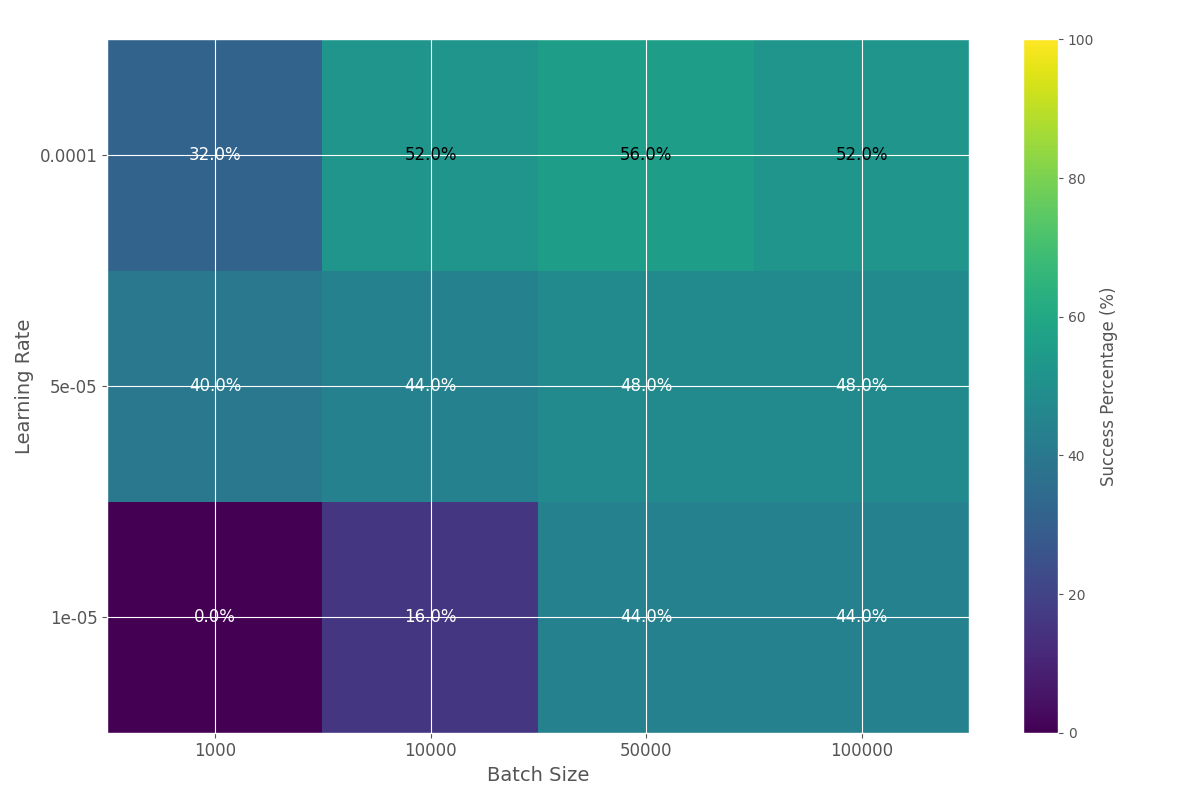
\includegraphics[width=0.8\textwidth]{imaxes/e_heatmap_MLP_RFMID.png}
    \caption{Mapa de calor cos resultados de diferentes combinacións de batch size e learning rate con unha mostra de imaxes de RMIFD ca función de activación ReLU}
    \label{fig:e_heatmap_MLP_RFMID}
\end{figure}

\paragraph{Discusión}
\label{par:Discusion-learningrate}

Valores de learning rate moi altos (0.001 and 0.005) son contraproducentes, xa que a rede diverxe rapidamente.

A dependencia entre o learning rate e o batch size confirmase. Xeralmente un learning rate baixo (1.0e-05, 1.0e-06) parece requerir de batch sizes maiores e viceversa, o cal é consistente co que se esperaba.

Tamén observase que batch sizes maiores tenden a dar mellores resultados.

\paragraph{Conclusións}
\label{par:Conclusions-learningrate}

\subsection{Batch size}
\label{subsec:Batch size}

\paragraph{Planteamento}
\label{par:Planteamento-batchsize}

Ao longo dos experimentos realizados, o análisis cualitativo revelou que o batch size é un dos parámetros que máis impacto ten no rendemento da rede.
Unha vez determinados uns valores aceptables nos parámetros anteriores, realizáronse experimentos para determinar cal era o batch size óptimo.

Neste caso dividimos o conxunto de datos de RFMID en varios subconxuntos según a dificultade da transformación, medida mediante a norma de Frobenius.
A norma de Frobenius dunha matriz $A \in \mathbb{R}^{m \times n}$ defínese como:

\[
\|A\|_F = \sqrt{\sum_{i=1}^{m} \sum_{j=1}^{n} |a_{ij}|^2}
\]

onde $a_{ij}$ son os elementos da matriz $A$.
Esta é unha xeralización da distancia euclidiana aplicada a matrices, onde as imaxes con transformacións mais grandes considéranse mais difíciles.

Desta forma podemos comparar o rendemento da rede en diferentes subconxuntos de imaxes, e determinar se o rendemento da rede é consistente entre eles.
Ademais, xa que a rede si que é capaz de rexistrar correctamente as imaxes dos subconxuntos mais sinxelos, utilizaremos a métrica de FIRE para medir o pocentaxe de imaxes rexistradas correctamente.

\paragraph{Resultados}
\label{par:Resultados-batchsize}

\ref{fig:batch_size_comparison_relu_1e-5}, \ref{fig:batch_size_comparison_relu_5e-5}, \ref{fig:batch_size_comparison_relu_1e-4}
\ref{fig:batch_size_comparison_siren_1e-4}, \ref{fig:batch_size_comparison_siren_1e-5}, \ref{fig:batch_size_comparison_siren_5e-5}

\begin{figure}[ht] 
    \centering
    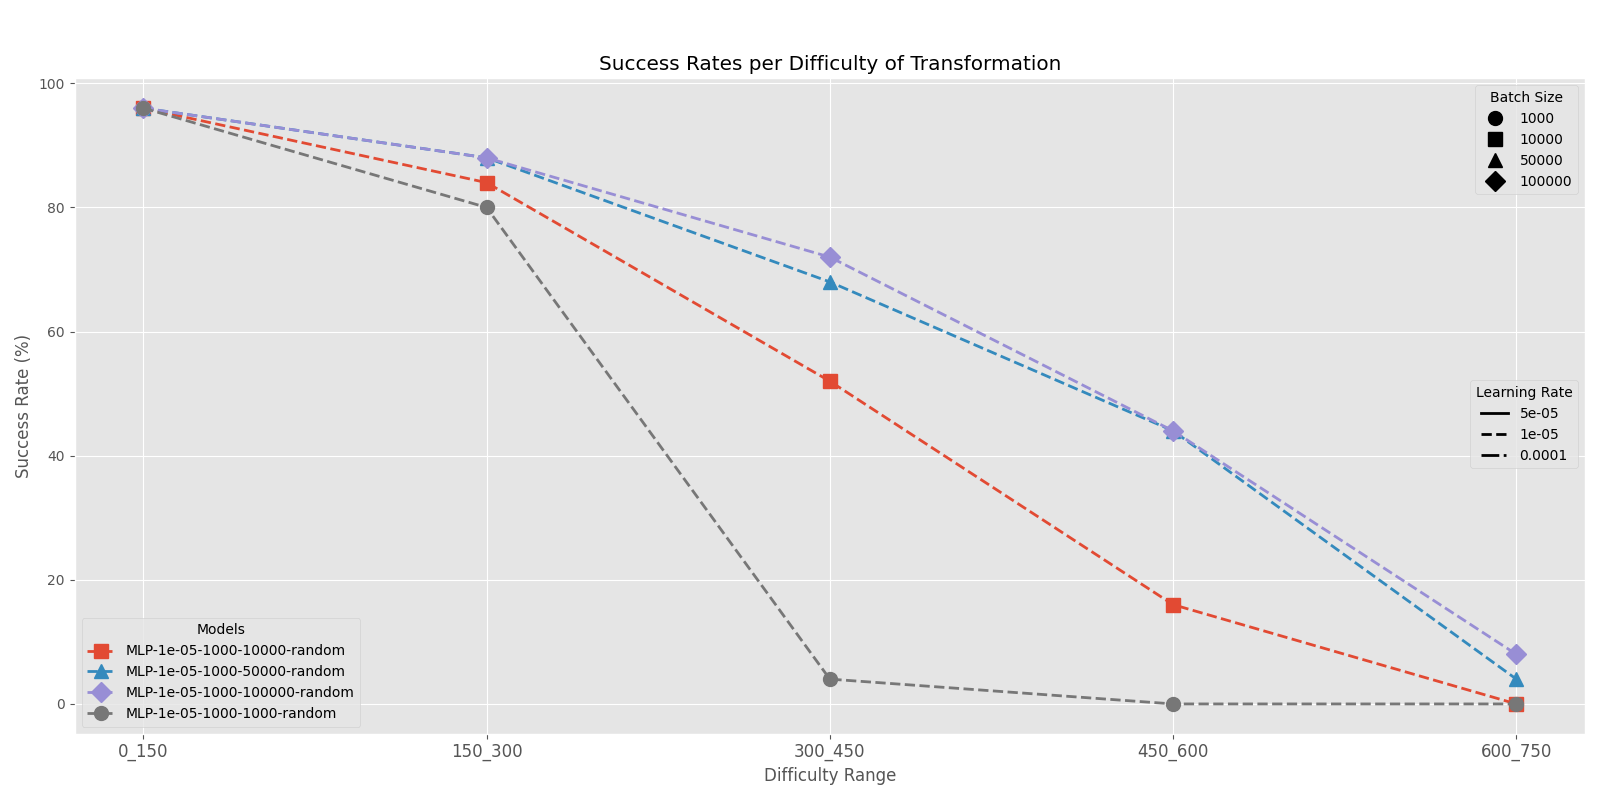
\includegraphics[width=0.8\textwidth]{imaxes/batchsize/experiment_plot_RFMID_MLP_1e-05.png}
    \caption{Comparación do rendemento da rede con diferentes batch sizes sobre imaxes do dataset RFMID ca función de activación ReLU (learning rate = 1e-5)}
    \label{fig:batch_size_comparison_relu_1e-5}
\end{figure}

\begin{figure}[ht] 
    \centering
    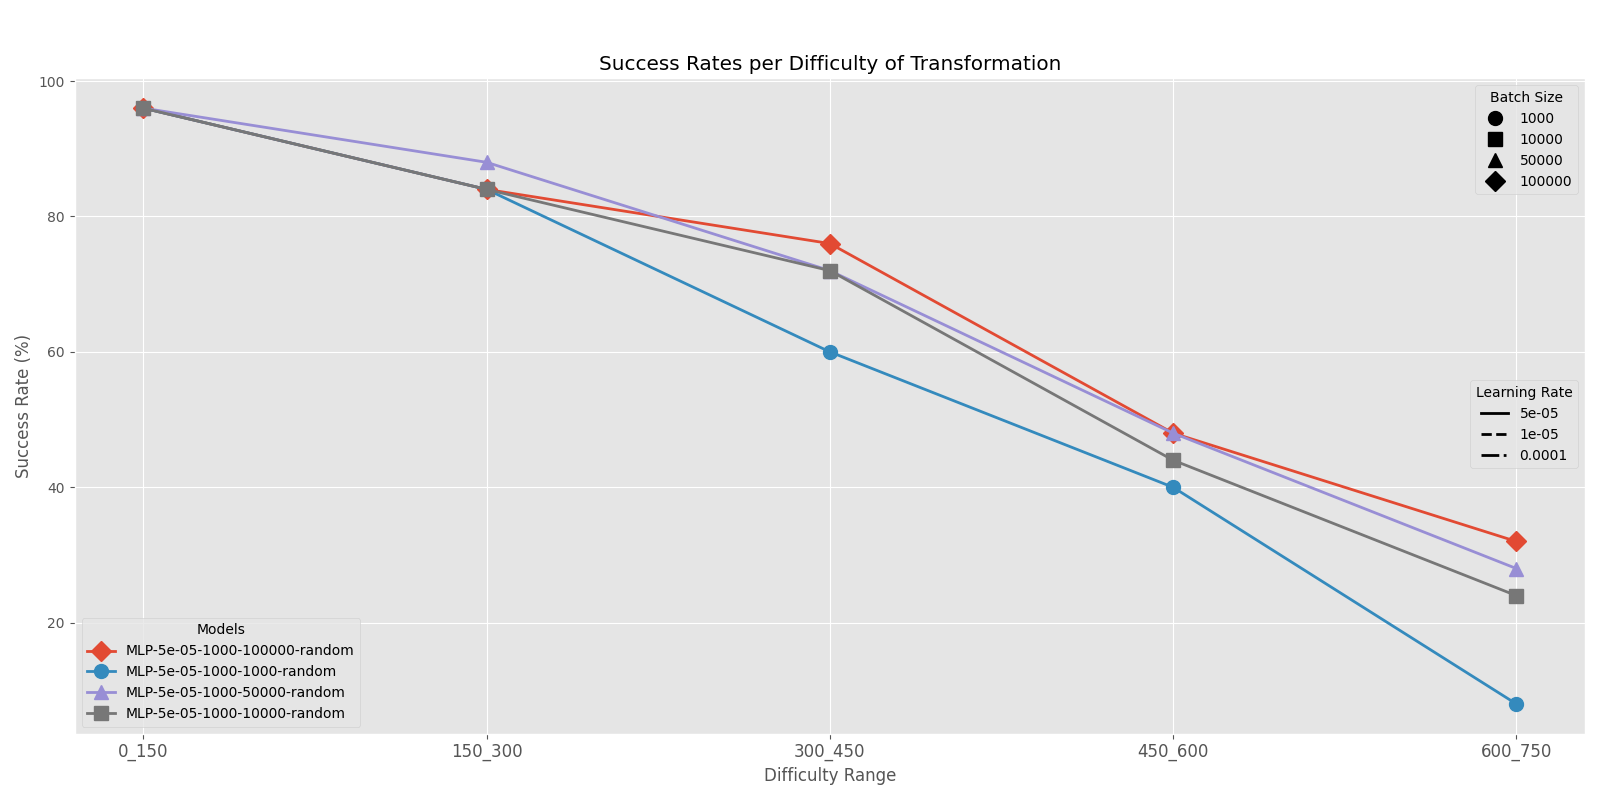
\includegraphics[width=0.8\textwidth]{imaxes/batchsize/experiment_plot_RFMID_MLP_5e-05.png}
    \caption{Comparación do rendemento da rede con diferentes batch sizes sobre imaxes do dataset RFMID ca función de activación ReLU (learning rate = 5e-5)}
    \label{fig:batch_size_comparison_relu_5e-5}
\end{figure}

\begin{figure}[ht] 
    \centering
    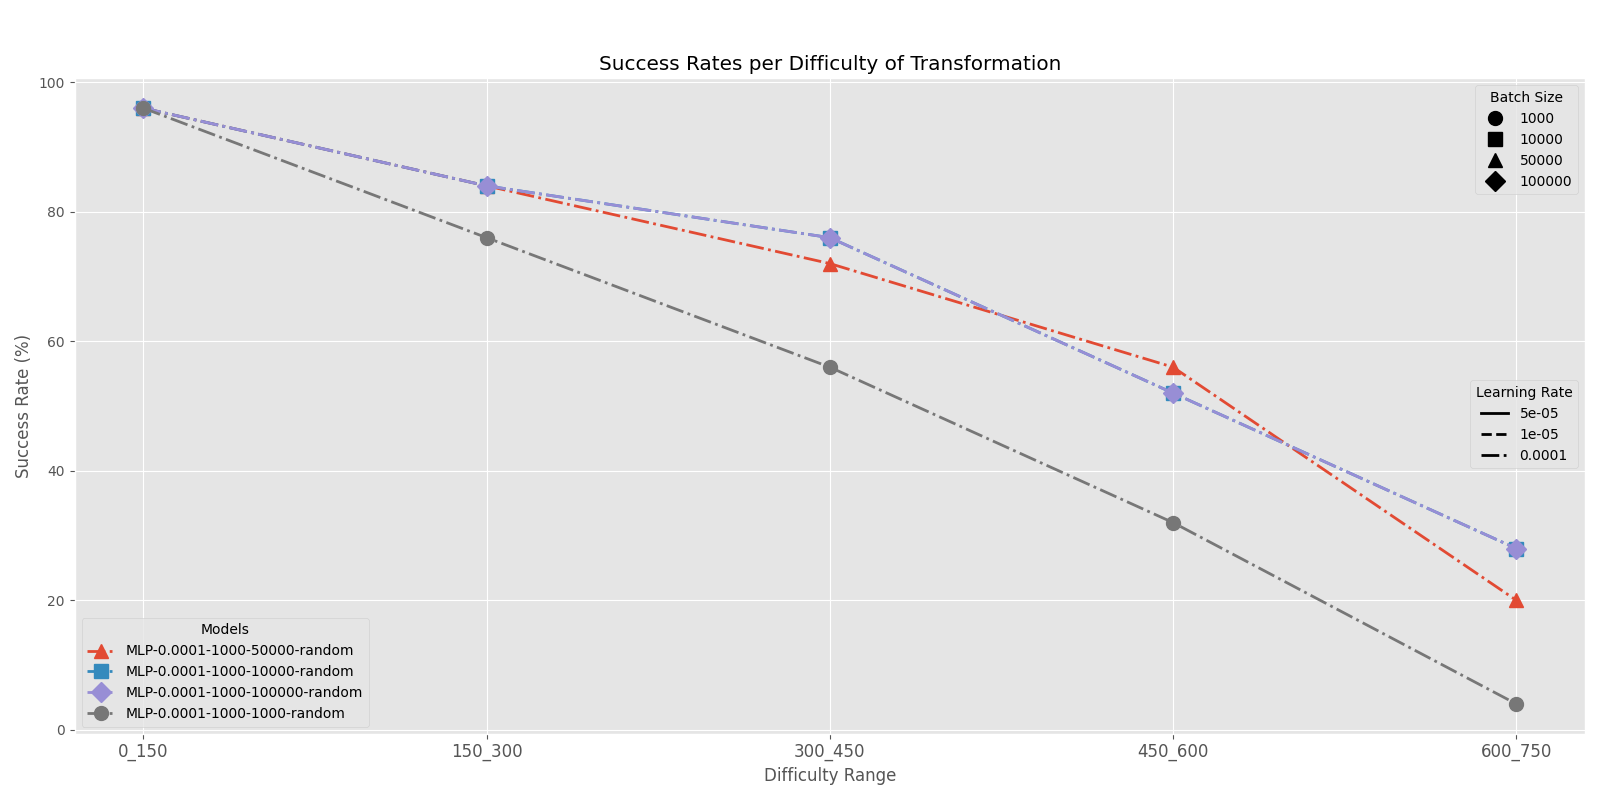
\includegraphics[width=0.8\textwidth]{imaxes/batchsize/experiment_plot_RFMID_MLP_0.0001.png}
    \caption{Comparación do rendemento da rede con diferentes batch sizes sobre imaxes do dataset RFMID ca función de activación ReLU (learning rate = 1e-4)}
    \label{fig:batch_size_comparison_relu_1e-4}
\end{figure}

\begin{figure}[ht] 
    \centering
    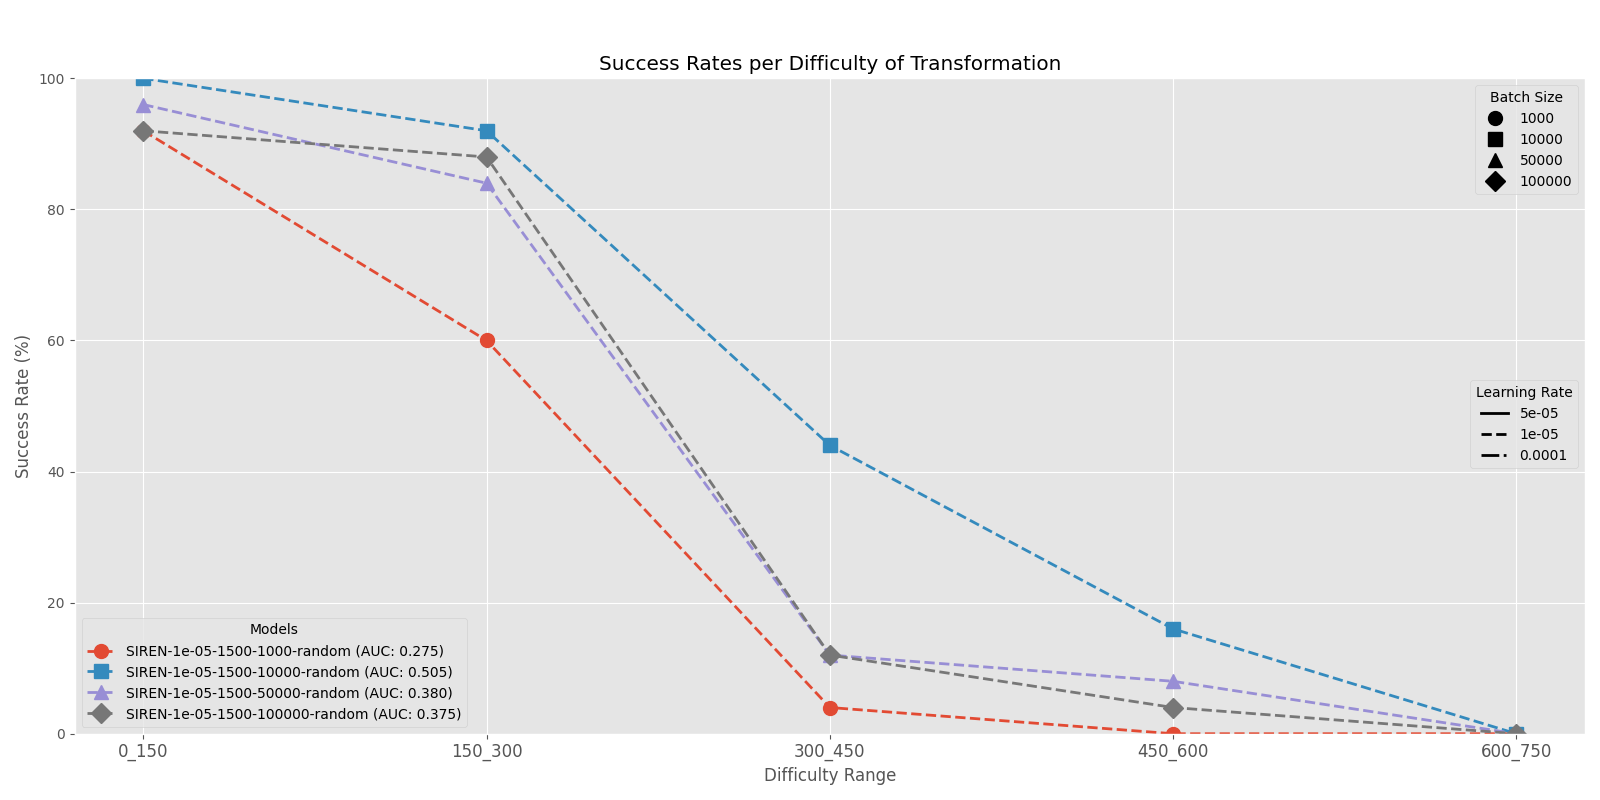
\includegraphics[width=0.8\textwidth]{imaxes/batchsize/experiment_plot_RFMID_SIREN_1e-05.png}
    \caption{Comparación do rendemento da rede con diferentes batch sizes sobre imaxes do dataset RFMID ca función de activación SIREN (learning rate = 1e-5)}
    \label{fig:batch_size_comparison_siren_1e-5}
\end{figure}

\begin{figure}[ht] 
    \centering
    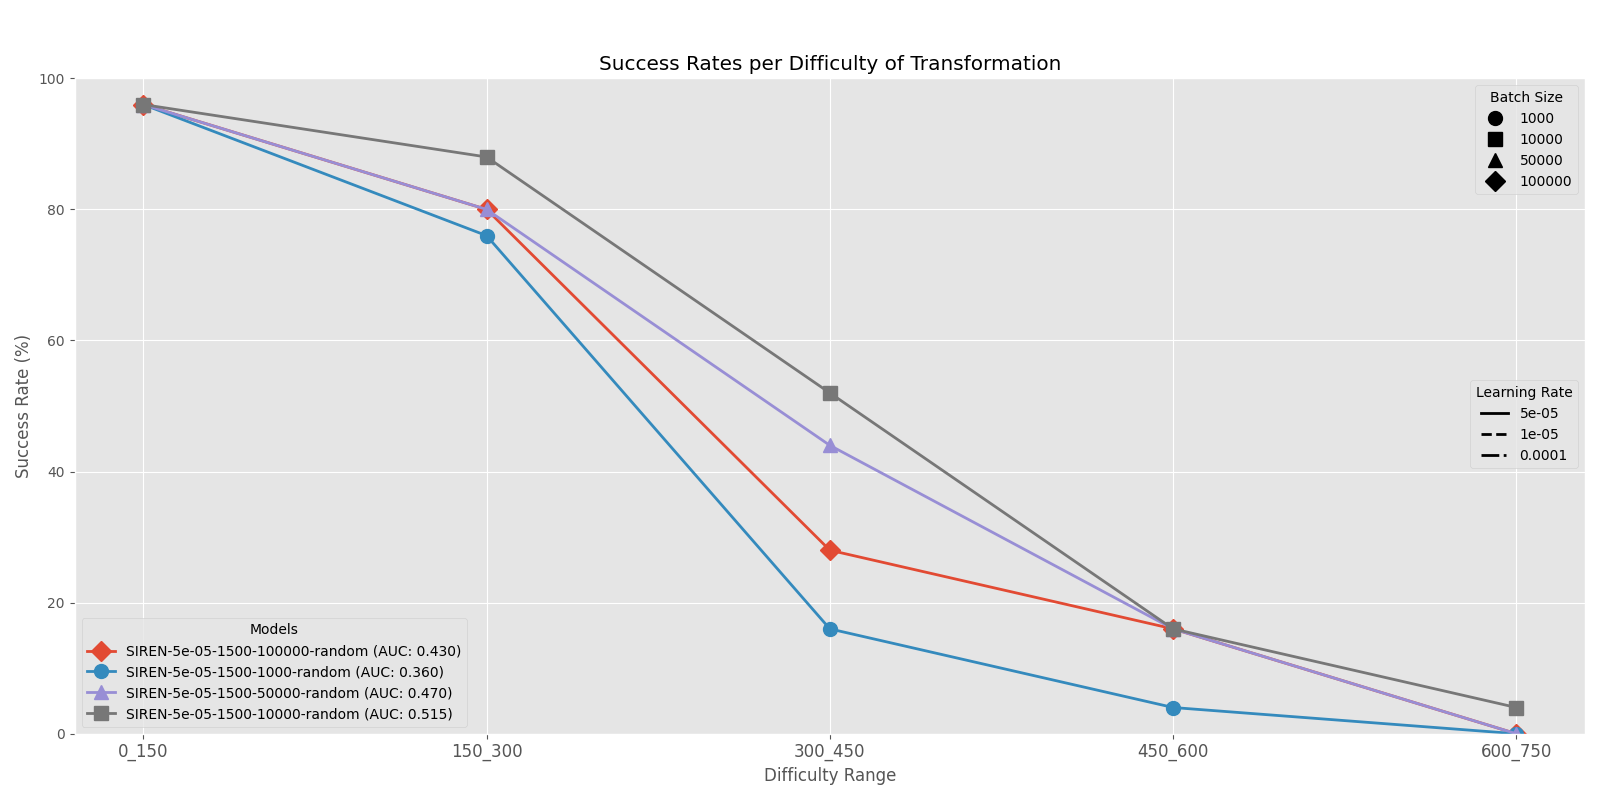
\includegraphics[width=0.8\textwidth]{imaxes/batchsize/experiment_plot_RFMID_SIREN_5e-05.png}
    \caption{Comparación do rendemento da rede con diferentes batch sizes sobre imaxes do dataset RFMID ca función de activación SIREN (learning rate = 5e-5)}
    \label{fig:batch_size_comparison_siren_5e-5}
\end{figure}

\begin{figure}[ht] 
    \centering
    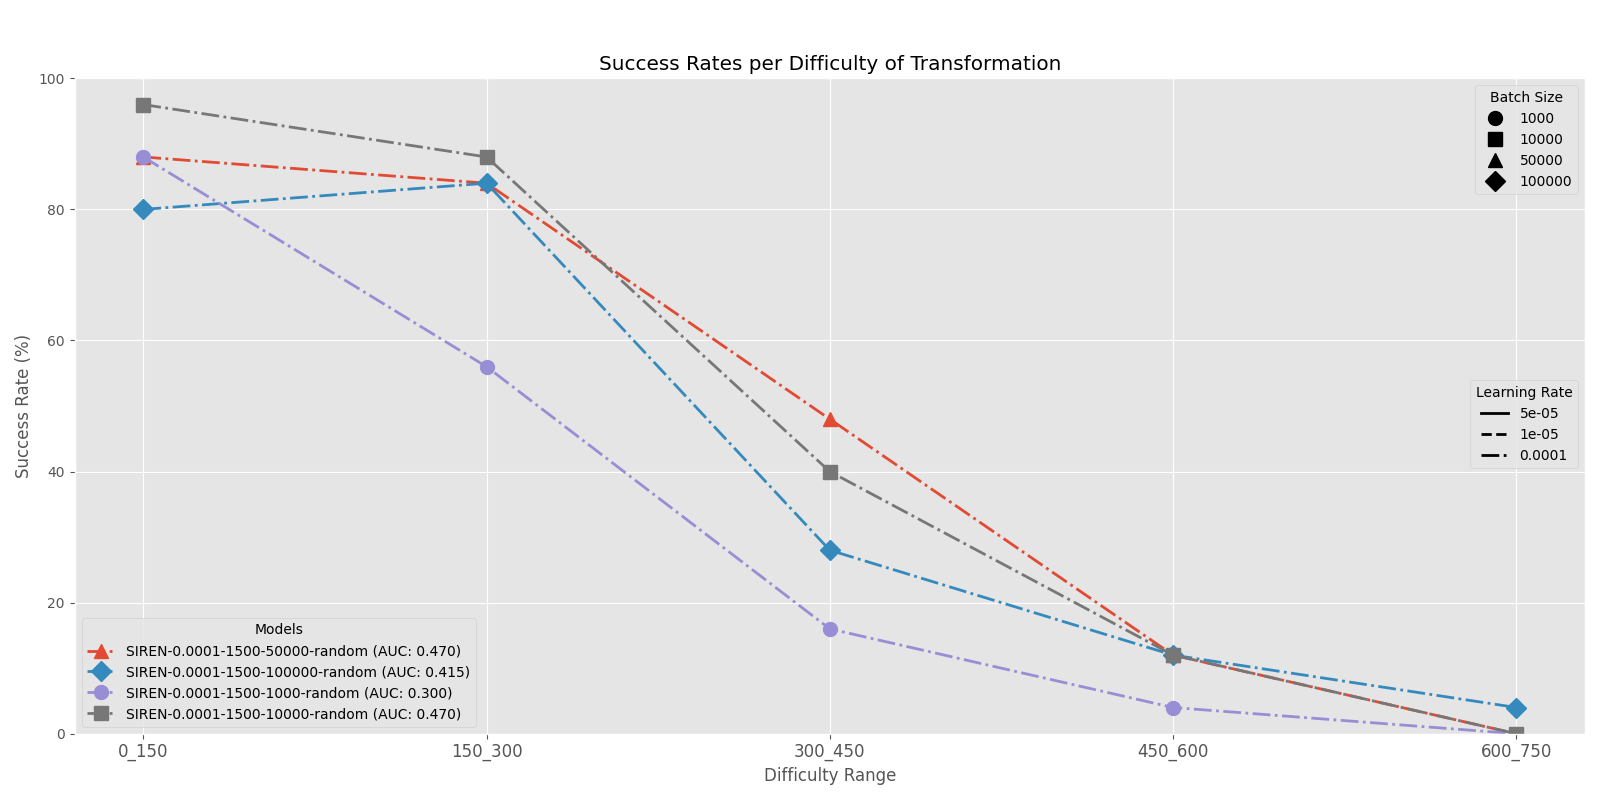
\includegraphics[width=0.8\textwidth]{imaxes/batchsize/experiment_plot_RFMID_SIREN_0.0001.png}
    \caption{Comparación do rendemento da rede con diferentes batch sizes sobre imaxes do dataset RFMID ca función de activación SIREN (learning rate = 1e-4)}
    \label{fig:batch_size_comparison_siren_1e-4}
\end{figure}


\paragraph{Discusión}
\label{par:Discusion-batchsize}

Obsérvase que as redes ca función de activación ReLU tenden a ter un rendemento moito mellor que as ca función de activación SIREN. Isto pode explicarse xa que as deformacións artificiais que se aplican nas imaxes do dataset RFMID son lineais, e a función de activación ReLU é adecuada para este tipo de transformacións.

Tamén parece que o batch size é relevante, especialmente o cambio entre 1000 e 10000, mentres que batch sizes maiores (50000, 100000) non parecen ter tanto impacto, aínda que si un maior custo computacional.

\paragraph{Conclusións}
\label{par:Conclusions-batchsize}

Interesa determinar cal é o punto de inflexión onde o aumento do batch size non compensa o aumento do rendemento.

\subsection{Estratexias de mostraxe}
\label{subsec:Estratexias de mostraxe}

Orixinalmente IDIR utiliza unha estratexia de mostraxe aleatoria para seleccionar os puntos que se pasan á rede en cada iteración.
Mentres que esta estratexia parece suficiente para o rexitro de pulmóns, no caso das imaxes de retina isto non ten porque ser así.
Isto débese a que as imaxes de retina conteñen seccións con moita mais información que outras, frente os CTs de pulmóns onde o sinal é mais uniforme.
Por exemplo, as seccións que conteñen vasos sanguíneos ou o disco óptico probablemente teñan mais información relevante para a tarefa de rexistro, frente outras seccións como o fondo da retina.
Ademais, as retinografías teñen desprazamentos moito maiores e menor superposición entre cada parella, polo que a rede ten que aprender transformacións mais complexas.

\paragraph{Planteamento}
\label{par:Planteamento-sampling}

Para solucionar isto, propúxose unha estratexia de mostraxe mais intellixente, onde se calcula unha máscara de probabilidade para cada imaxe, que se utiliza para seleccionar os puntos que se pasan á rede.
Para calcular esta máscara, extráense mediante operadores de Sobel os vasos sanguíneos e mediante umbralización o disco óptico, que son as zonas onde se espera que haxa máis información, e dáselles maiores probabilidades de ser seleccionadas.

Posteriormente tamén se introducíu unha estratexia de mostraxe uniforme, onde se seleccionan un número fixo de puntos en cada imaxe.
É unha estratexia similar ao mostraxe aleatorio, pero garantindo que se cubre a maior parte posible da imaxe. Isto é relevante en experimentos con batch sizes pequenos onde unha mostraxe aleatoria non ten por que cubrir toda a imaxe de forma uniforme.
Para implementalo empregouse unha distribución baseada na grella de Fibonacci (Fibonacci lattice), que permite repartir os puntos de maneira uniforme sobre a superficie circular da retina. 
A posición de cada punto calcúlase en coordenadas polares, asignando a cada punto un radio proporcional á raíz cadrada do seu índice dividido polo número total de puntos, e un ángulo proporcional ao índice multiplicado por $2\pi$ e dividido polo cadrado do número áureo ($\varphi^2$):

\[
r_i = \sqrt{\frac{i}{N}}, \quad \theta_i = 2\pi \frac{i}{\varphi^2}
\]

onde $i$ é o índice do punto ($i = 1, \dots, N$), $N$ é o número total de puntos e $\varphi$ é o número áureo. 
Deste xeito, conséguese unha cobertura uniforme e eficiente da rexión de interese, evitando agrupamentos ou zonas baleiras.

Así mesmo implementouse un scheduling do batch size, ca idea de utilizar un batch size pequeno nos epochs iniciais para que a rede aprenda unha transformación global a grandes rasgos, e aumentar o número de puntos conforme avanza o entrenamento para que a rede aprenda as transformación locais.
A estratexia de mostraxe uniforme é a mais axeitada para este caso, especialmente cando se utiliza un batch size pequeno.
O learning rate modificaráse de forma proporcional para manter a relación entre ambos.

Na figura \ref{fig:sampling_heatmaps} pódense observar os diferentes tipos de mostraxe utilizados.

\begin{figure}[ht]
    \centering
    \begin{subfigure}[b]{0.3\textwidth}
        \centering
        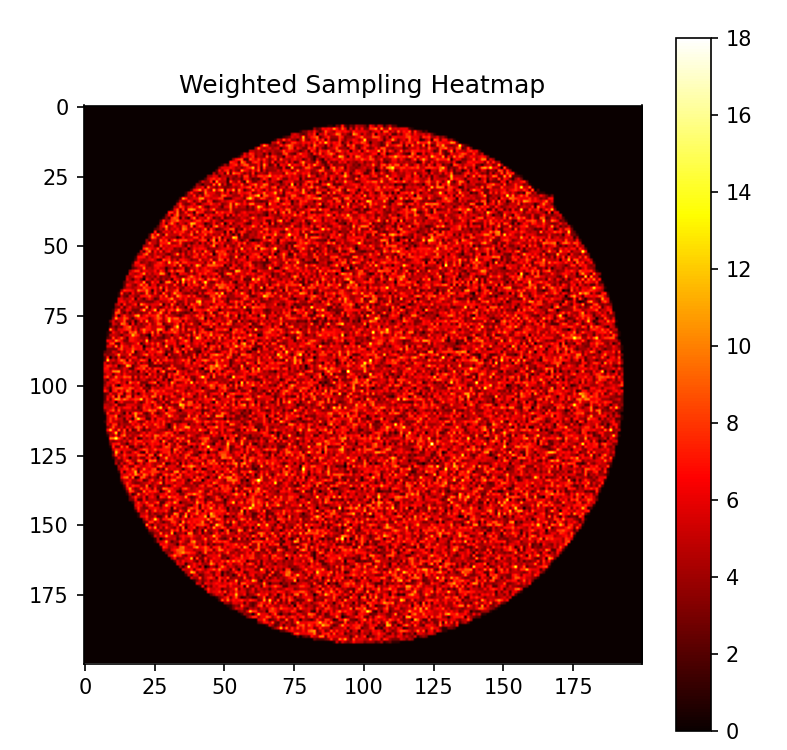
\includegraphics[width=\textwidth]{imaxes/muestraje/random_sampling_heatmap.png}
        \caption{Heatmap de mostraxe aleatorio}
        \label{fig:random_sampling_heatmap}
    \end{subfigure}
    \hfill
    \begin{subfigure}[b]{0.3\textwidth}
        \centering
        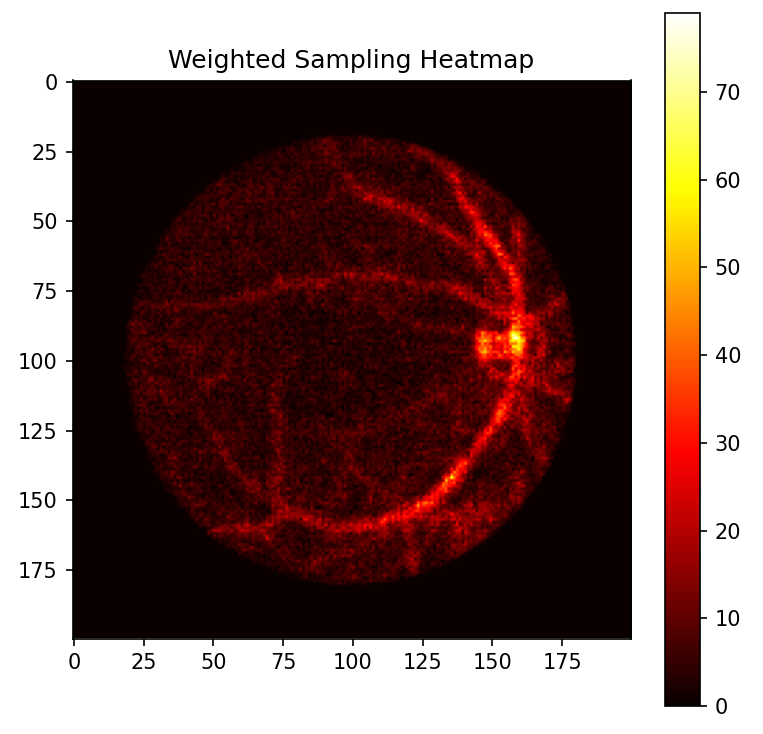
\includegraphics[width=\textwidth]{imaxes/muestraje/weighted_sampling_heatmap.png}
        \caption{Heatmap de mostraxe con peso}
        \label{fig:weighted_sampling_heatmap}
    \end{subfigure}
    \hfill
    \begin{subfigure}[b]{0.3\textwidth}
        \centering
        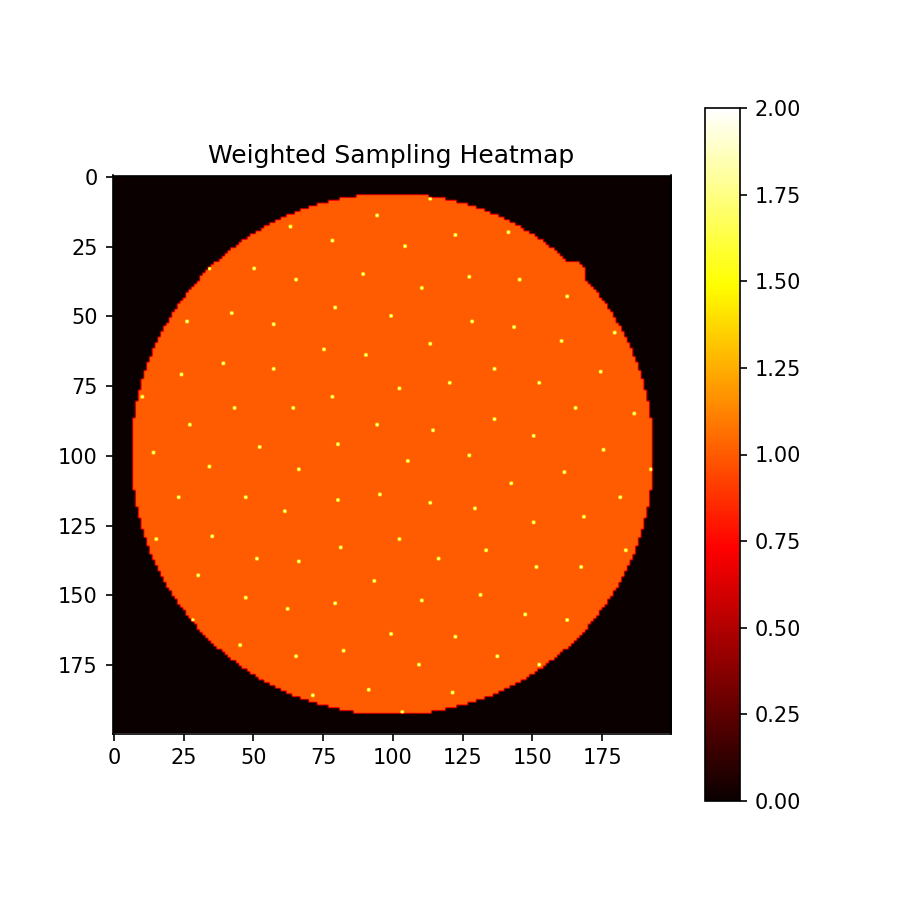
\includegraphics[width=\textwidth]{imaxes/muestraje/uniform_sampling_heatmap.png}
        \caption{Heatmap de mostraxe uniforme (100 puntos)}
        \label{fig:uniform_sampling_heatmap}
    \end{subfigure}
    \caption{Heatmaps de mostraxe}
    \label{fig:sampling_heatmaps}
\end{figure}


\paragraph{Resultados}
\label{par:Resultados-sampling}

\ref{fig:sampling_comparison}
\ref{fig:fire_samplingtype}
\ref{fig:sampling_comparison_relu}
\ref{fig:sampling_comparison_SIREN}
\begin{figure}[ht]
    \centering
    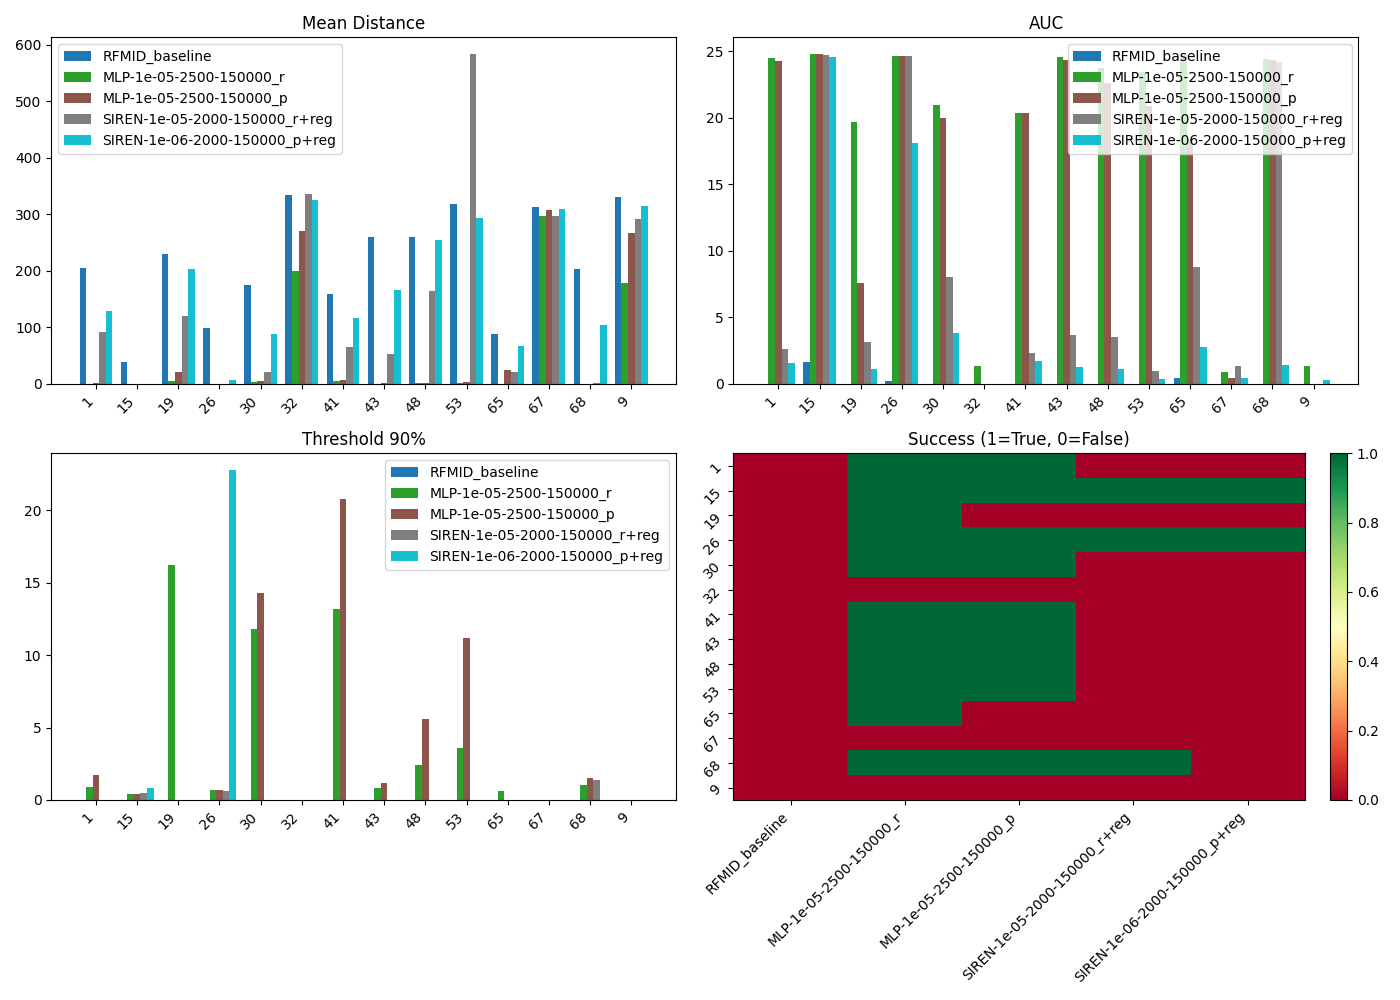
\includegraphics[width=0.8\textwidth]{imaxes/muestraje/RFMID_both__comp_sampling.png}
    \caption{Comparación das diferentes estratexias de mostraxe sobre imaxes do dataset RFMID}
    \label{fig:sampling_comparison}
\end{figure}

\begin{figure}[ht]
    \centering
    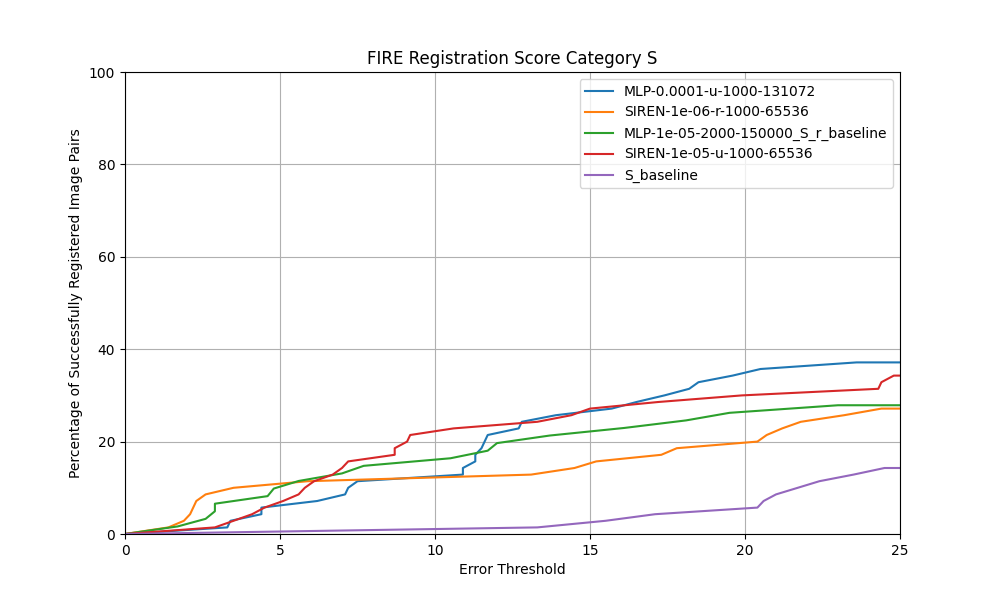
\includegraphics[width=0.8\textwidth]{imaxes/muestraje/fire_samplingtype.png}
    \caption{Comparación das diferentes estratexias de mostraxe sobre imaxes do dataset FIRE}
    \label{fig:fire_samplingtype}
\end{figure}


\begin{figure}[ht]
    \centering
    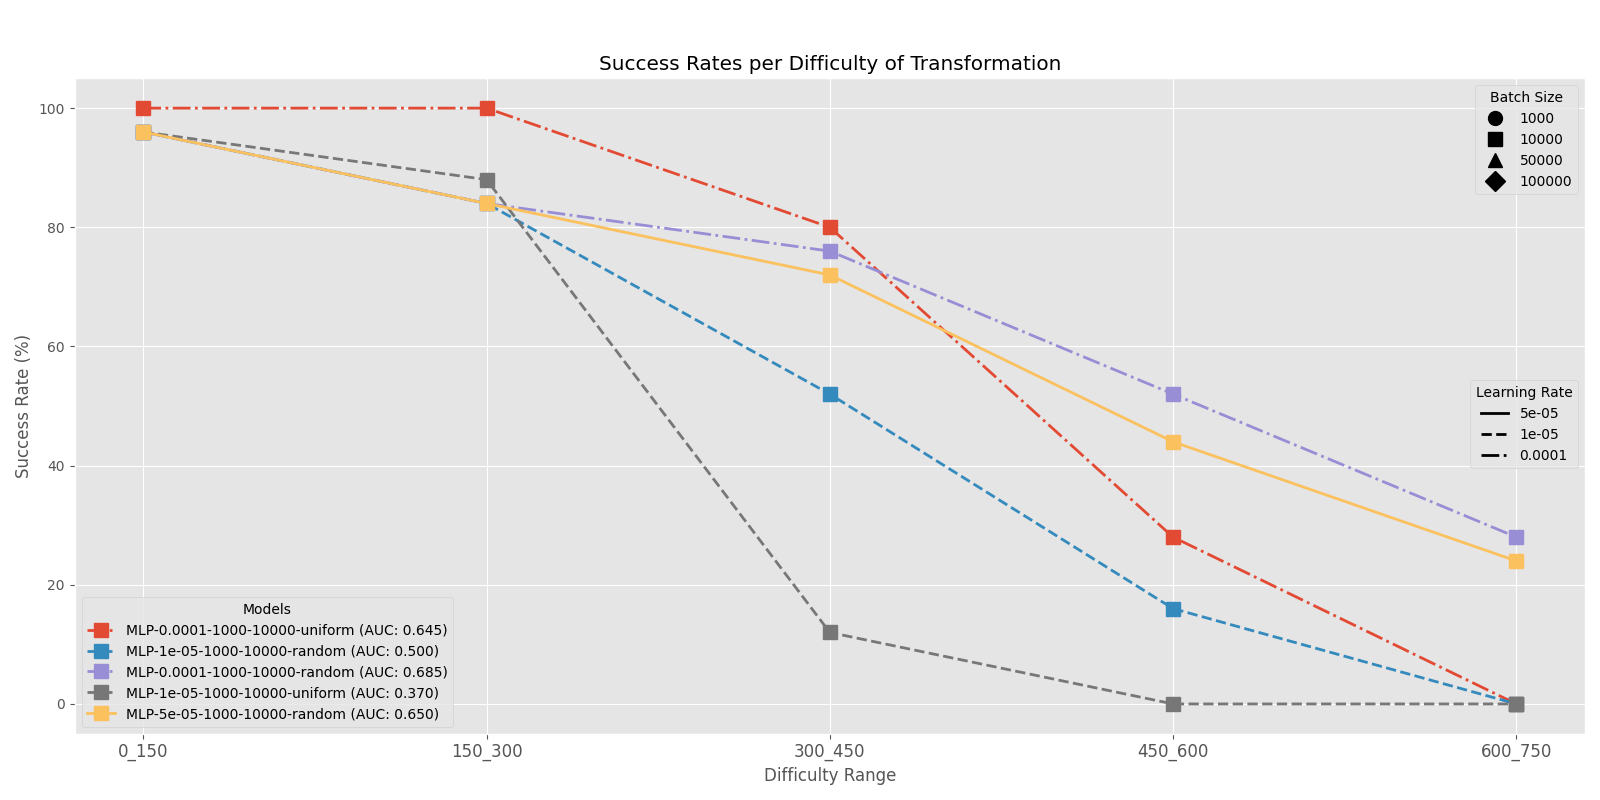
\includegraphics[width=0.8\textwidth]{imaxes/muestraje/experiment_plot_RFMID_MLP_RvsU.png}
    \caption{Comparación das diferentes estratexias de mostraxe sobre imaxes do dataset RFMID ca función de activación RELU}
    \label{fig:sampling_comparison_relu}
\end{figure}

\begin{figure}[ht]
    \centering
    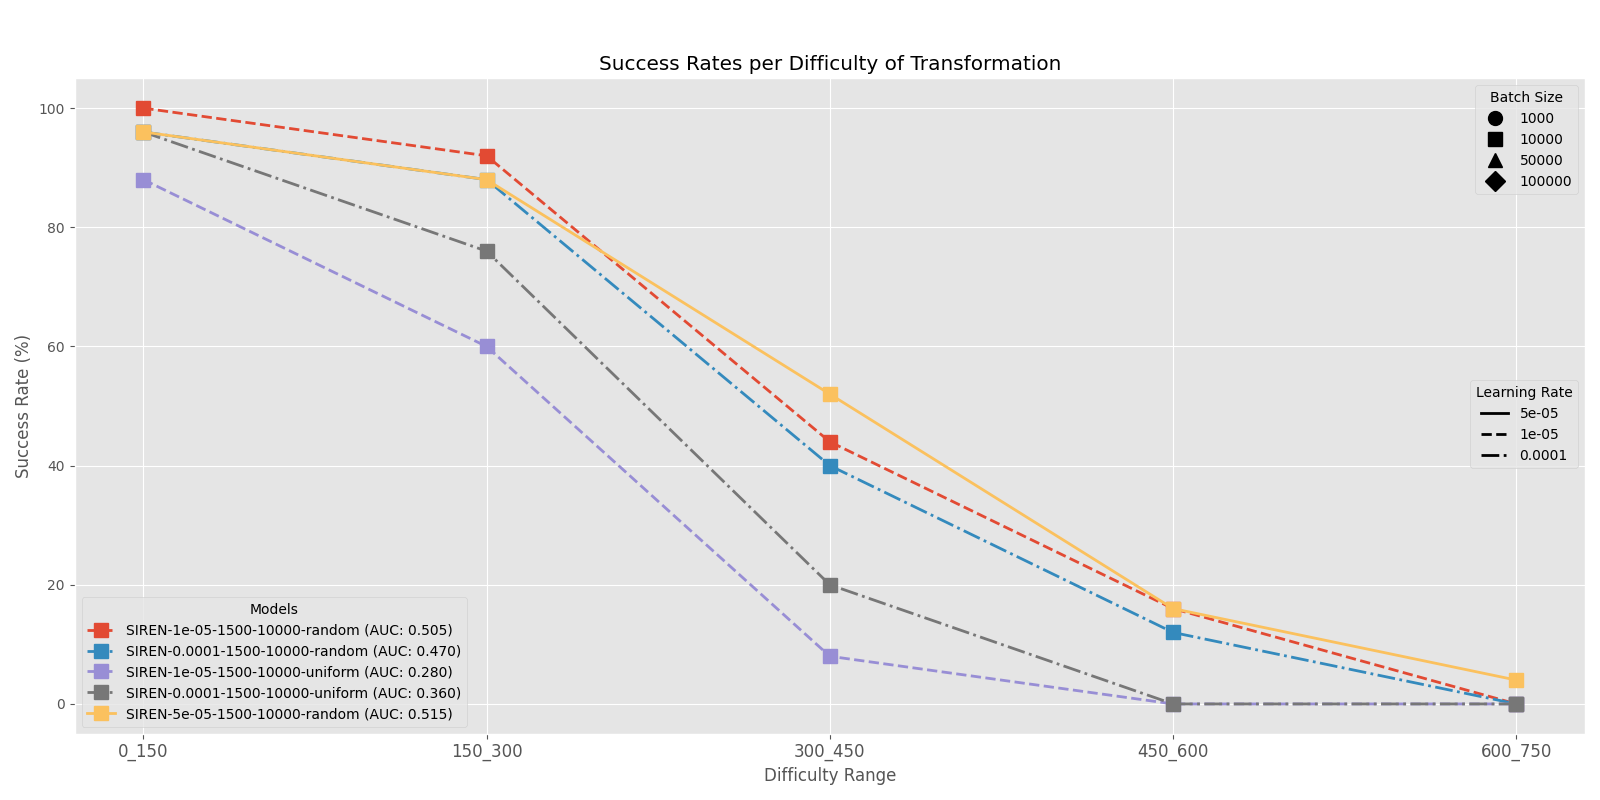
\includegraphics[width=0.8\textwidth]{imaxes/muestraje/experiment_plot_RFMID_SIREN_RvsU.png}
    \caption{Comparación das diferentes estratexias de mostraxe sobre imaxes do dataset RFMID ca función de activación SIREN}
    \label{fig:sampling_comparison_SIREN}
\end{figure}



\paragraph{Discusión}
\label{par:Discusion-sampling}

A hipótese da estratexia de mostraxe intellixente non parece ser a mais axeitada, con resultados peores ca estratexia aleatoria. 
A estratexia uniforme tampouco parece ser a mais adecuada, xa que non se obtén resultados significativamente mellores ca a aleatoria.


\paragraph{Conclusións}
\label{par:Conclusions-sampling}

\subsection{Inicialización}
\label{subsec:Inicialización}

\paragraph{Planteamento}
\label{par:Planteamento-initialization}

É posible que a inicialización da rede sexa un factor mais importante que a estratexia de mostraxe. É posible que certas inicializacións coloquen os despraszamentos de forma que a rede sexa incapaz de aprender a transformación correcta, ou que lle custe moito mais aprenderla.

Para testar esta hipótese implementouse unha lotería de inicialización, onde se utiliza o loss no epoch 0 para determinar a inicialización da rede mais beneficiosa.
É posible que fore mellor esperar ata un epoch algo mais avanzado para determinar a inicialización, xa que no epoch 0 non hay ningunha seguridade de que non sexa un mínimo local, pero isto tamén implicaría un maior custo computacional.

\paragraph{Resultados}
\label{par:Resultados-initialization}

\ref{fig:lottery_initial_deformations_combinedMLP}, \ref{fig:lottery_initial_deformations_combinedSIREN}

\ref{fig:lottery}

\begin{figure}[ht]
    \centering
    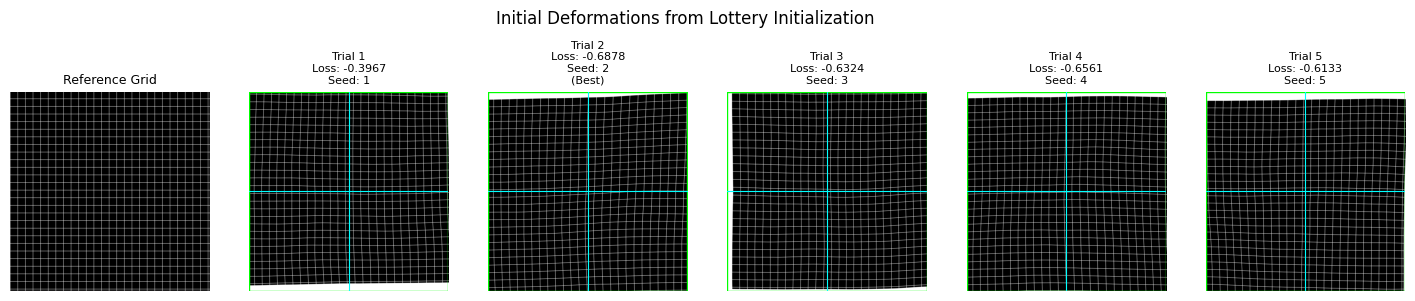
\includegraphics[width=0.8\textwidth]{imaxes/lottery/initial_deformations_combinedMLP.png}
    \caption{Exemplos das diferentes inicializacións ca función de activación RELU}
    \label{fig:lottery_initial_deformations_combinedMLP}
\end{figure}

\begin{figure}[ht]
    \centering
    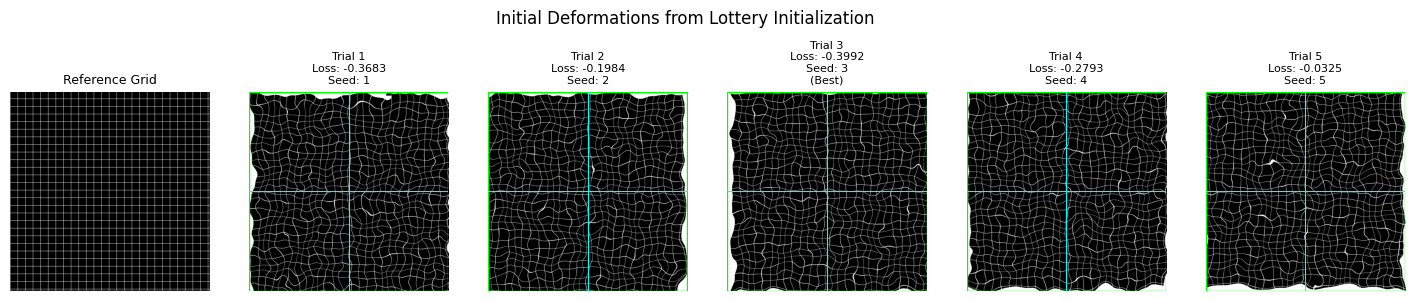
\includegraphics[width=0.8\textwidth]{imaxes/lottery/initial_deformations_combinedSIREN.png}
    \caption{Exemplos das diferentes inicializacións ca función de activación SIREN}
    \label{fig:lottery_initial_deformations_combinedSIREN}
\end{figure}


\begin{figure}[ht]
    \centering
    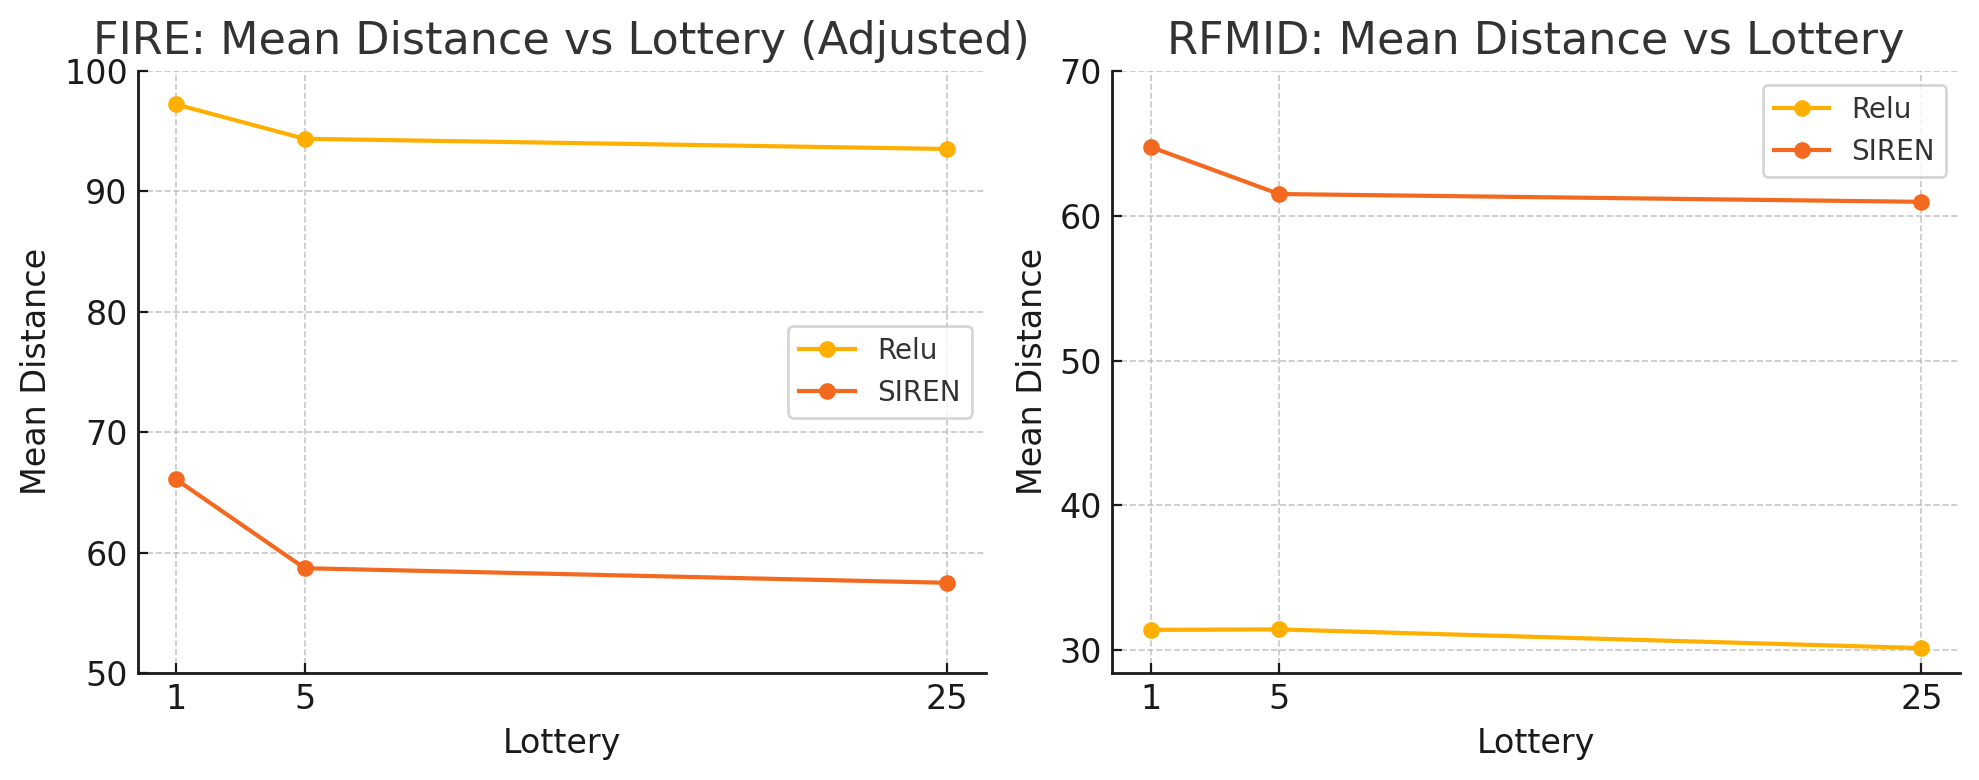
\includegraphics[width=0.8\textwidth]{imaxes/lottery/lotery.png}
    \caption{Resultados da lotería de inicialización}
    \label{fig:lottery}
\end{figure}

\paragraph{Discusión}
\label{par:Discusion-initialization}

Obsérvase que a lotería de inicialización si que provoca unha mellora, aínda que non moi significativa, e non se beneficia particularmente de utilizar mais de 5 inicializacións.

\paragraph{Conclusións}
\label{par:Conclusions-initialization}

Unha posible mellora á lotería de inicialización sería utilizar un número maior de epochs antes de determinar a inicialización gañadora, xa que o loss inicial non é necesariamente representativo do rendemento final da rede.
Poderíase tamén determinar como de sensible é a rede a diferentes inicializacións.

\subsection{Fases}
\label{subsec:Fases}
\paragraph{Planteamento}
\label{par:Planteamento-phases}

Teorízase que a rede pode beneficiarse de dividir o proceso de rexistro en diferentes fases, onde inicialmente utilízase un batch size reducido para aprender a transformación global, e posteriormente aumentase o batch size para aprender as transformacións locais.
Para isto utilizaremos a estratexia de mostraxe uniforme, que permite asegurar que se cubre toda a imaxe de forma uniforme, o que é mais importante con batch sizes pequenos.

\paragraph{Resultados}
\label{par:Resultados-phases}

\ref{fig:nphases}, 
\begin{figure}[ht]
    \centering
    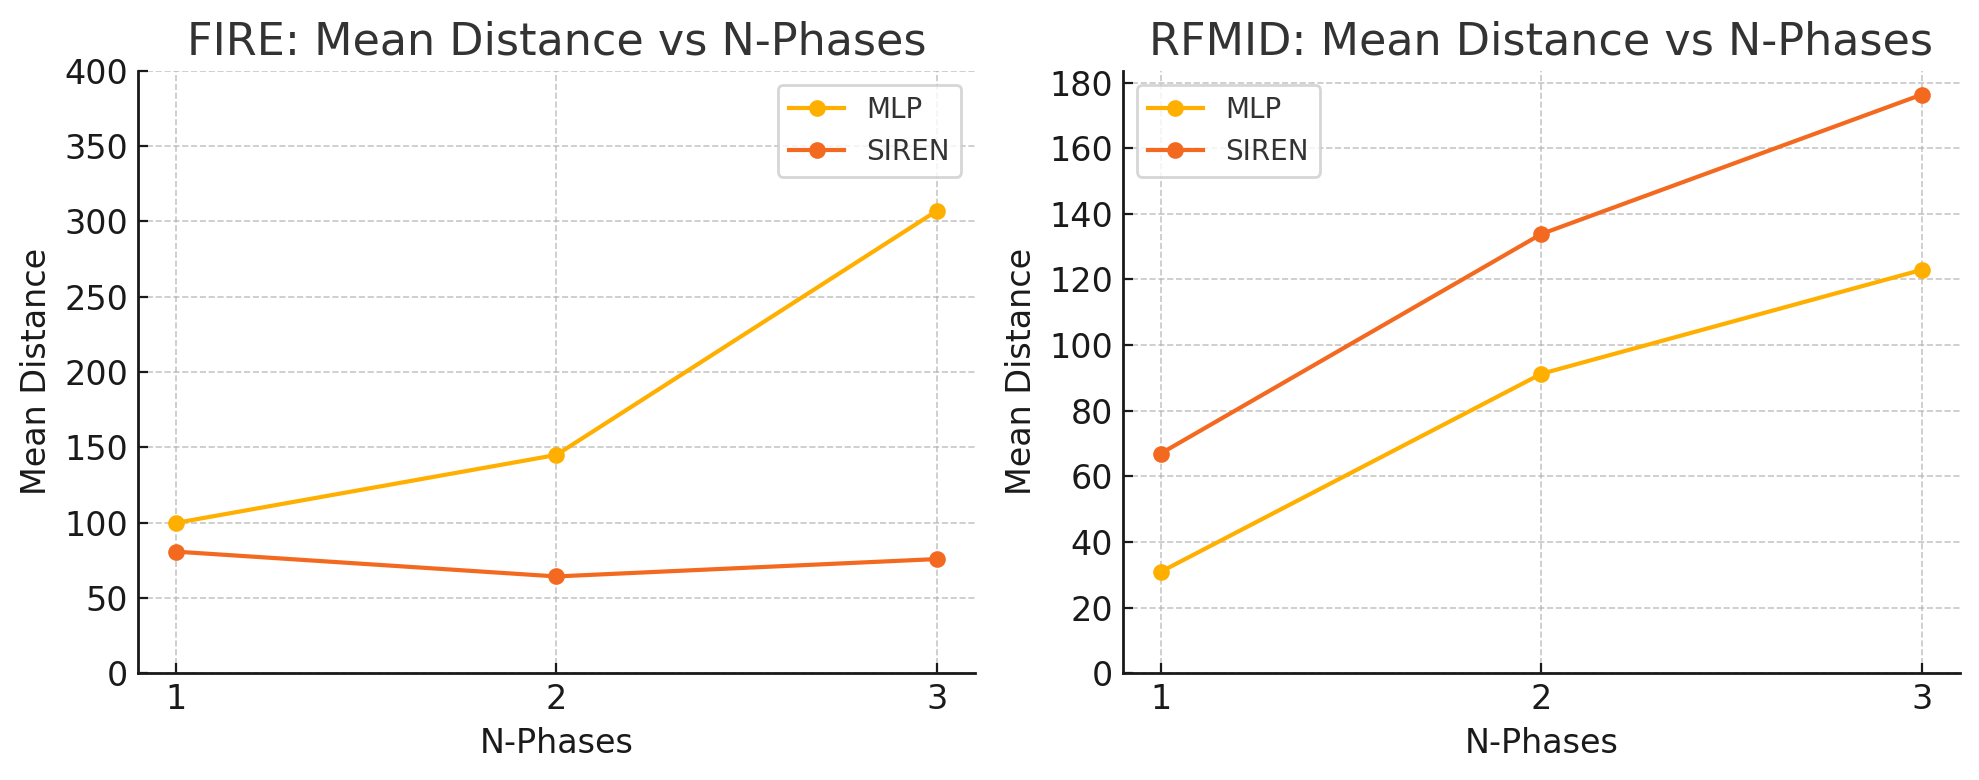
\includegraphics[width=0.8\textwidth]{imaxes/lottery/nphases.png}
    \caption{Resultados de usar distinto número de fases}
    \label{fig:nphases}
\end{figure}

\paragraph{Discusión}
\label{par:Discusion-phases}

A hipótese parece errada, xa que o uso de fases tende a empeorar o rendemento da rede.
Isto pode deberse a que a rede xa é capaz de aprender as transformacións globais e locais simultaneamente, ou que a hipótese de que un menor batch size ayuda a aprender as transformacións globais non é correcta.

\paragraph{Conclusións}
\label{par:Conclusions-phases}


\subsection{Exemplos de rexistro}
\label{subsec:Exemplos de rexistro}

\ref{fig:reg_examples}

Estes exemplos ilustran o resultado do rexistro de diferentes imaxes, mostrando tanto rexistros exitosos como fallidos.
A primeira imaxe corresponde ca imaxe fixa, a segunda corresponde ca imaxe rexistrada, a terceira ca imaxe móbil e a cuarta o campos de deformación aplicado a unha gralla cadrada.

Pódense observar os puntos de control, sendo os blancos os da imaxe fixa, os verdes os da imaxe móbil e os azuis os desprazados pola rede.
\begin{figure}[ht]
    \centering
    \begin{subfigure}[b]{0.45\textwidth}
        \centering
        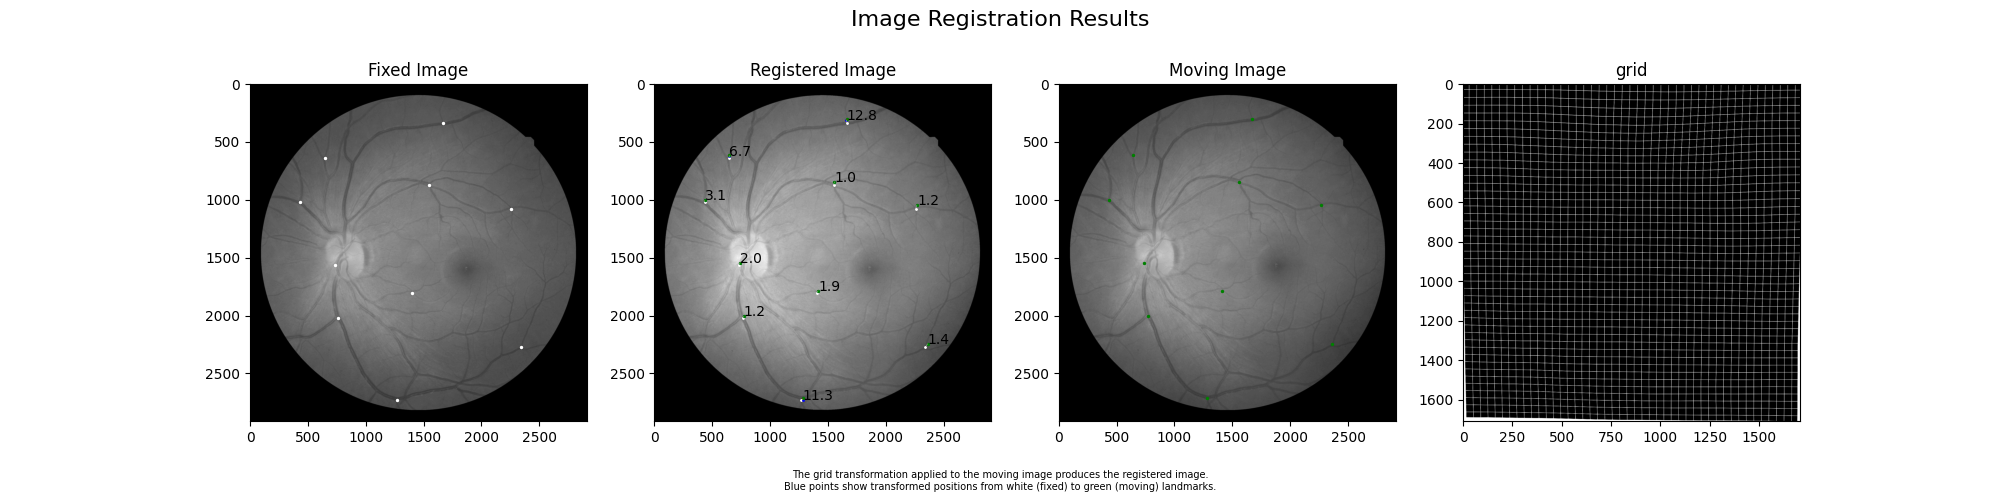
\includegraphics[width=\textwidth]{imaxes/reg_examples/FIRE_MLP_buena.png}
        \caption{Rexistro exitoso dunha parella de imaxes do dataset FIRE ca función de activación ReLU}
        \label{fig:reg_example_FIRE_MLP_buena}
    \end{subfigure}\hfill
    \begin{subfigure}[b]{0.45\textwidth}
        \centering
        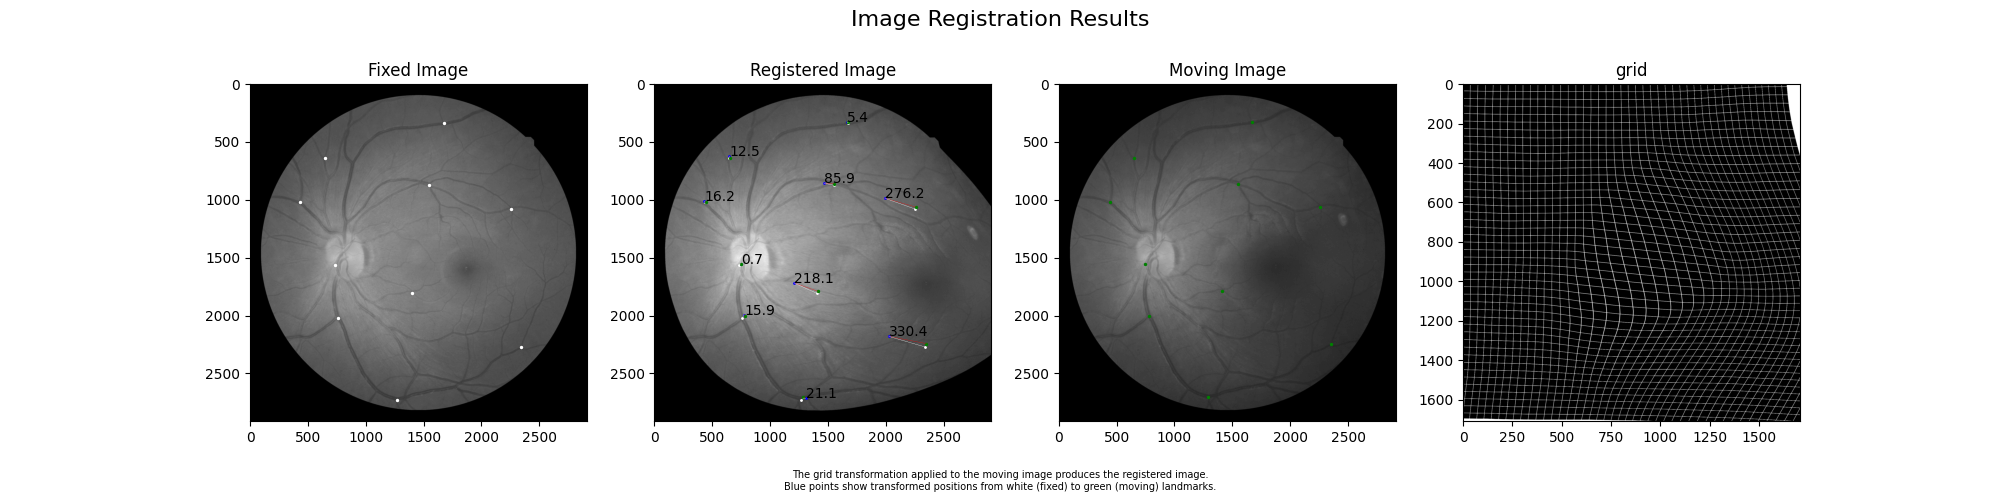
\includegraphics[width=\textwidth]{imaxes/reg_examples/FIRE_MLP_mala.png}
        \caption{Rexistro fallido dunha parella de imaxes do dataset FIRE ca función de activación ReLU}
        \label{fig:reg_example_FIRE_MLP_mala}
    \end{subfigure}

    \vskip\baselineskip

    \begin{subfigure}[b]{0.45\textwidth}
        \centering
        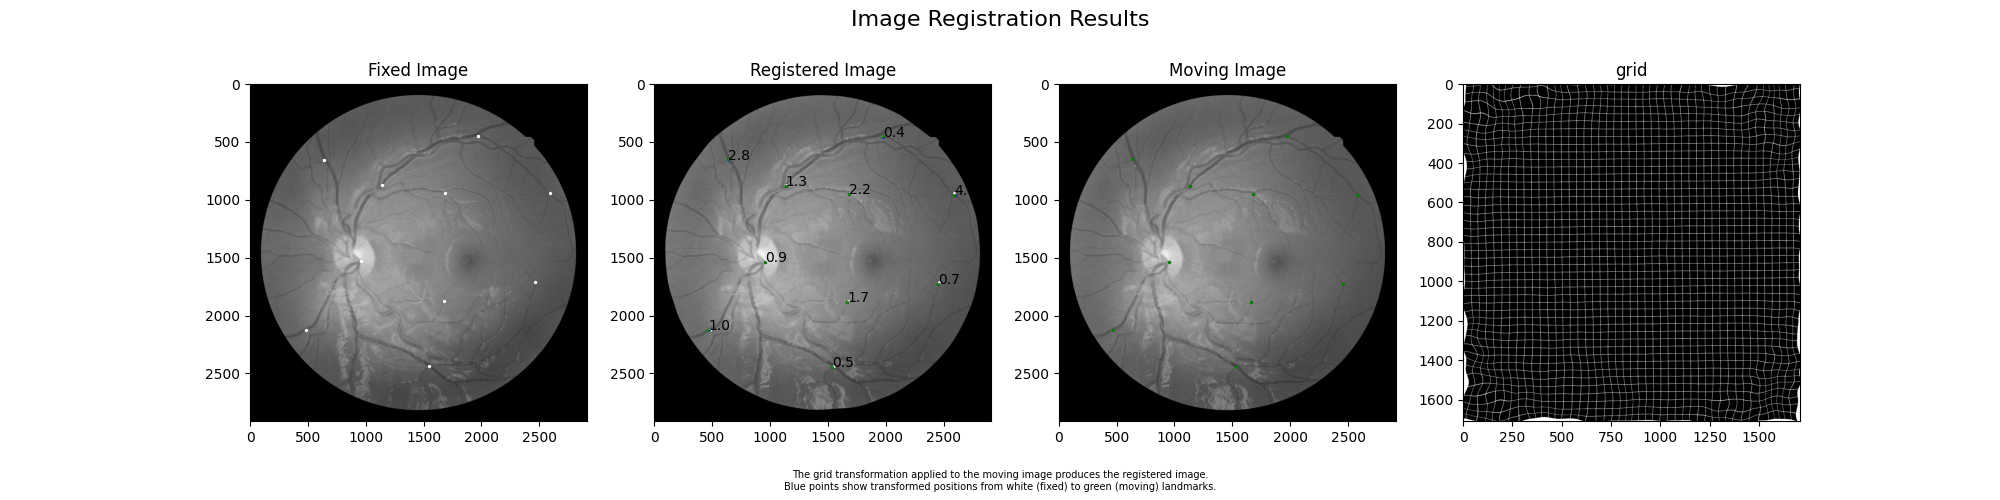
\includegraphics[width=\textwidth]{imaxes/reg_examples/FIRE_SIREN_buena.png}
        \caption{Rexistro exitoso dunha parella de imaxes do dataset FIRE ca función de activación SIREN}
        \label{fig:reg_example_FIRE_SIREN_buena}
    \end{subfigure}\hfill
    \begin{subfigure}[b]{0.45\textwidth}
        \centering
        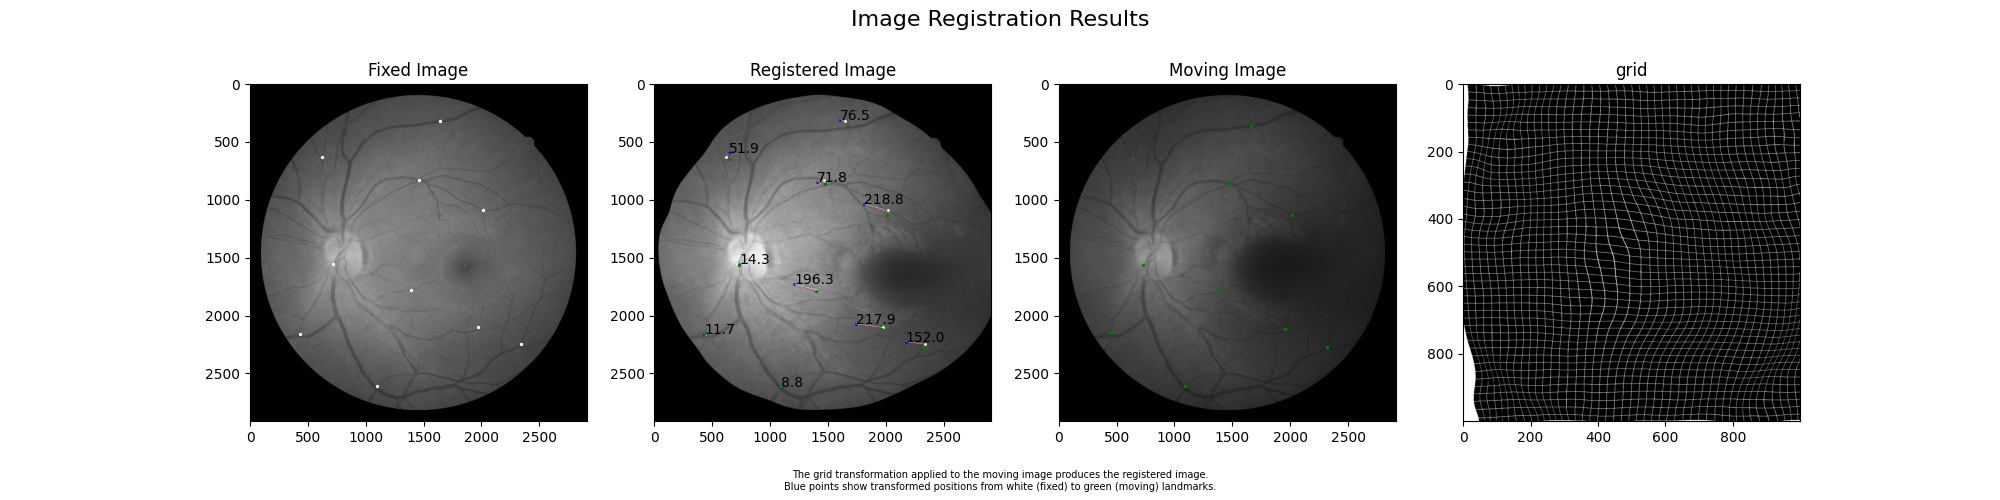
\includegraphics[width=\textwidth]{imaxes/reg_examples/FIRE_SIREN_mala.png}
        \caption{Rexistro fallido dunha parella de imaxes do dataset FIRE ca función de activación SIREN}
        \label{fig:reg_example_FIRE_SIREN_mala}
    \end{subfigure}

    \vskip\baselineskip

    \begin{subfigure}[b]{0.45\textwidth}
        \centering
        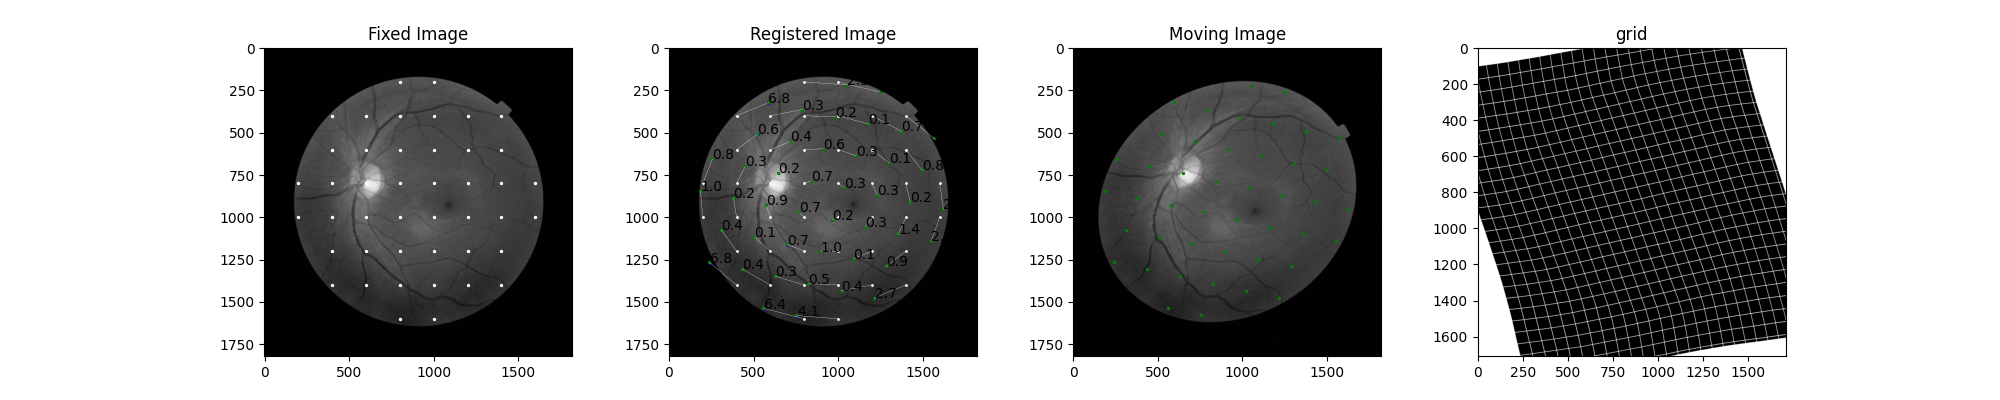
\includegraphics[width=\textwidth]{imaxes/reg_examples/RFMID_MLP_buena.png}
        \caption{Rexistro exitoso dunha parella de imaxes do dataset RFMID ca función de activación ReLU}
        \label{fig:reg_example_RFMID_MLP_buena}
    \end{subfigure}\hfill
    \begin{subfigure}[b]{0.45\textwidth}
        \centering
        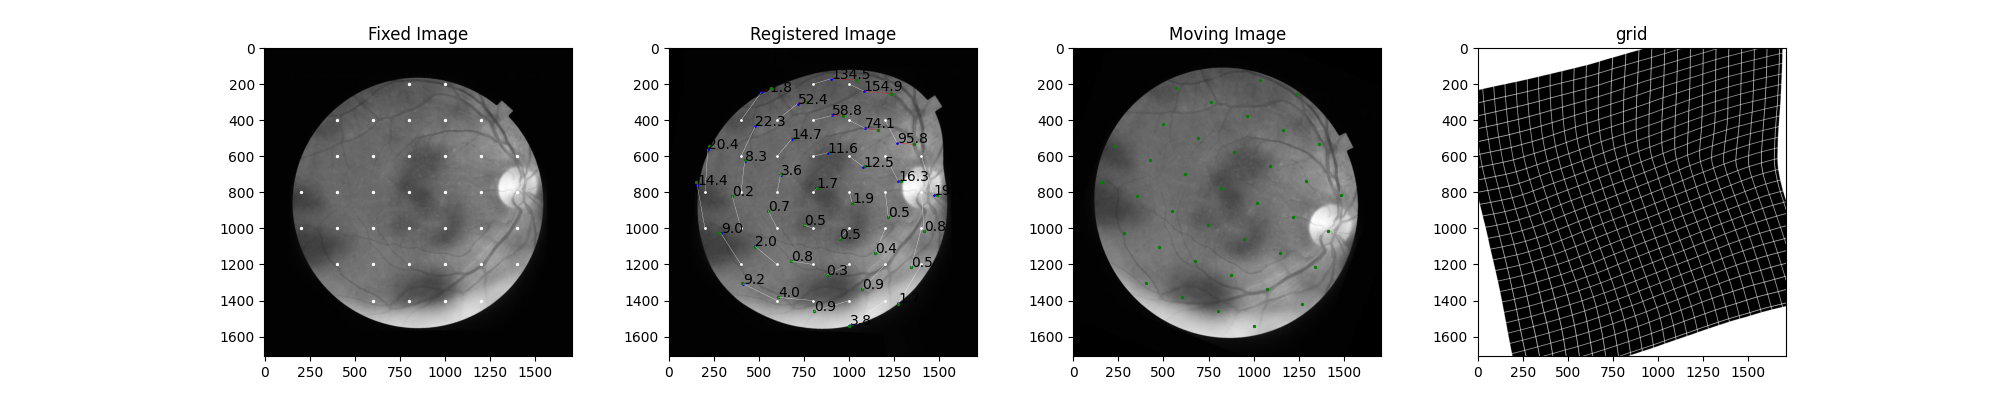
\includegraphics[width=\textwidth]{imaxes/reg_examples/RFMID_MLP_mala.png}
        \caption{Rexistro fallido dunha parella de imaxes do dataset RFMID ca función de activación ReLU}
        \label{fig:reg_example_RFMID_MLP_mala}
    \end{subfigure}

    \vskip\baselineskip

    \begin{subfigure}[b]{0.45\textwidth}
        \centering
        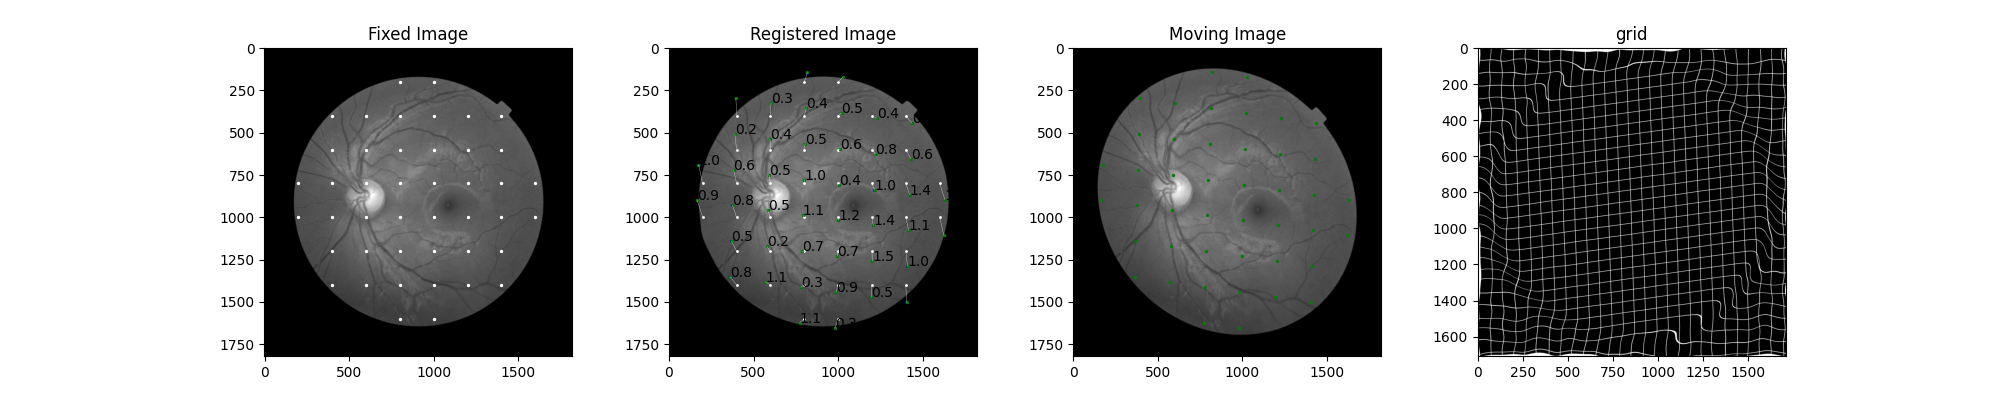
\includegraphics[width=\textwidth]{imaxes/reg_examples/RFMID_SIREN_buena.png}
        \caption{Rexistro exitoso dunha parella de imaxes do dataset RFMID ca función de activación SIREN}
        \label{fig:reg_example_RFMID_SIREN_buena}
    \end{subfigure}\hfill
    \begin{subfigure}[b]{0.45\textwidth}
        \centering
        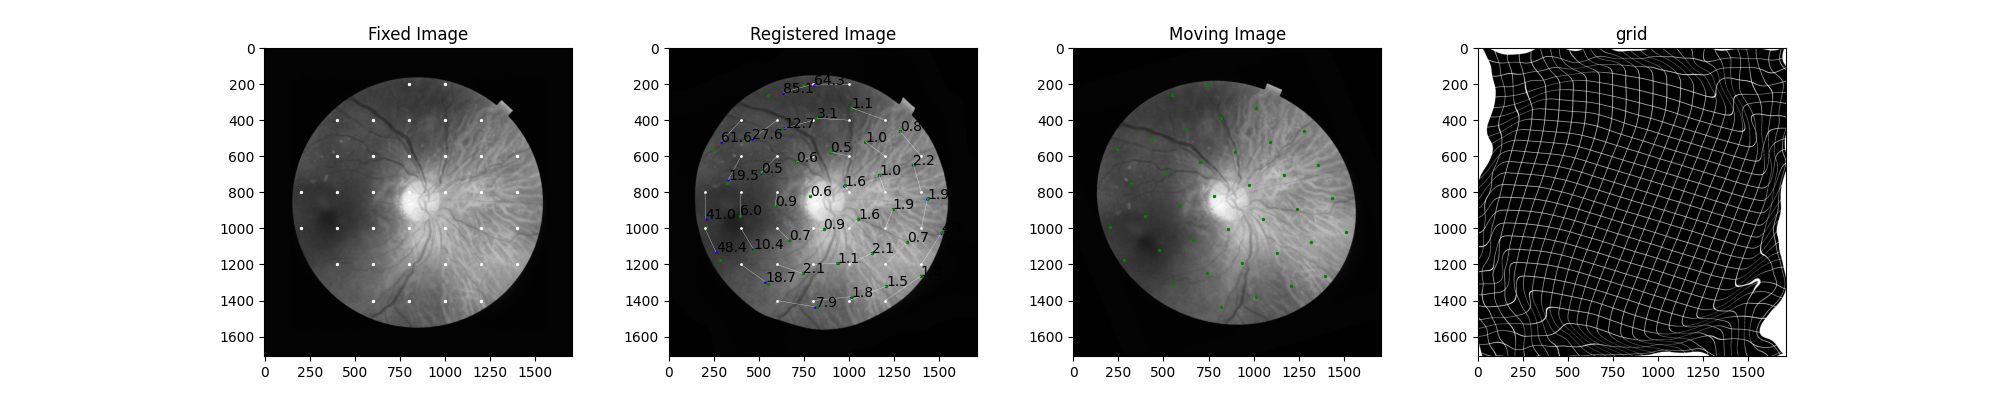
\includegraphics[width=\textwidth]{imaxes/reg_examples/RFMID_SIREN_mala.png}
        \caption{Rexistro fallido dunha parella de imaxes do dataset RFMID ca función de activación SIREN}
        \label{fig:reg_example_RFMID_SIREN_mala}
    \end{subfigure}

    \caption{Exemplos de rexistro: combinacións de dataset (FIRE/RFMID), función de activatción (relu/SIREN) e éxito.}
    \label{fig:reg_examples}
\end{figure}
  \chapter{Conclusións}
\label{chap:Conclusións}

\lettrine{E}{n} conclusión, o proxecto de investigación realizado consistiu na adaptación do framework IDIR para o rexistro de retinografías.
En especial valoramos o uso da función de activación SIREN, proposta como alternativa á función ReLU para mellorar a representación das deformacións.

A aliñación de retinografías é un problema relevante xa que é un proceso laborioso para os expertos, mais con moita uilidade clínica.
A etapa inicial da revisión do estado da arte revelou que xa existían varios traballos previos que abordaban este problema, sendo os máis exitosos os baseados en métodos iterativos.
Actualmente os métodos de aprendizaxe profunda son unha alternativa prometedora que está gañando prominencia no campo. Particularmente, o uso de representacións implícitas para esta tarefa é un enfoque innovador que xa foi aplicado en outros campos da imaxe médica con bós resultados.

Para avaliar a efectividade do método proposto, escolléronse dous conxuntos de datos de retinografías: FIRE, que permite a avaliación do método en imaxes reais, e RFMID, sobre o que se efectuaron transformacións artificiais para simular diferentes escenarios de aliñación.

Durante a fase de experimentación exploráronse diferentes combinacións de hiperparámetros (loss, regularización, resolución, batch size...) e introducíronse diferentes técnicas para tentar mellorar a converxencia do modelo, como diferentes esquemas de mostraxe, inicialización, e técnicas de axuste dinámico do batch size.

Algunhas das dificultades atopadas durante o desenrrolo do proxecto foron: a falta de documentación sobre o funcionamento do código orixinal, que dificultou a súa adaptación ao novo dominio; o deseño do proceso de avaliación, no cal foi complexo atopar visualizacións que permitisen interpretar os resultados facilmente; e o tempo de cómputo que requerían algúns experimentos, que requeriu a implementación de optimizacións para facilitar a experimentación.

Os resultados obtidos amosan que esta arquitectura non é a máis adecuada para a tarefa de rexistro de retinografías.

Si que se obteñen bós resultados no dataset RFMID, que se basea en imaxes con transformacións lineais sintéticas, onde a función de activación ReLU tende a obter mellores resultados ca SIREN, xa que está mellor preparada para representar as transformacións lineais globais que se producen entre estas imaxes.
Obsérvase tamén que o tamaño da transformación ten un impacto significativo no rendemento, xa que as imaxes de maior tamaño presentan un maior erro de rexistro.

No dataset FIRE, que contén imaxes reais, os resultados son peores ca no dataset RFMID, especialmente nas parellas de imaxes que presentan grandes deformacións ou baixo nivel de superposición.
A función de activación SIREN obtén mellores resultados aquí, xa que é capaz de representar mellor as deformacións non lineais e locais que se producen entre as imaxes.

Estas diferencias no rendemento destacan a importancia da elección da función de activación en función da natureza específica das transformacións esperadas.
A fase de experimentación tamén revelou que a regularización é un factor fundamental, especialmente na función de activación SIREN, onde a ausencia de regularización leva a un sobreaxuste significativo e a un rendemento moi pobre.

Cabe destacar que o método presentado neste traballo guía a optimización con tan só a métrica de NCC, que depende únicamente das intensidades dos píxeles, e que en rexitros con moito desprazamento ou deformacións complexas a topografía de función de perda será pouco convexa e con múltiples mínimos locais, o que dificulta a converxencia do modelo.
Polo contrario, métodos como REMPE \cite{rempe} que obteñen resultados moito mellores (rexistra exitosamente a totalidade da categoría S de FIRE) fan uso de información adicional que lles permite establecer correspondencias globais entre as imaxes.

Unha observación relevante é a diferencia entre o rendemento entre o conxunto de datos sintético (RFMID) e o conxunto de datos real (FIRE). Esta brecha demostra a dificultade de aplicar modelos adestrados en datos sintéticos a imaxes reais.

Todos estes achados responden aos obxectivos propostos no inicio do proxecto, onde adaptamos o framework IDIR para o rexistro de retinografías, exploramos a función de activación SIREN e avaliamos o rendemento do modelo en diferentes condicións.

  \chapter{Traballo futuro}
\label{chap:Traballo futuro}

\lettrine{E}{xisten} varias liñas de traballo futuro que se poden seguir para mellorar o sistema actual.
 Os resultados obtidos neste traballo, aínda que demostran a viabilidade de adaptar o framework IDIR para o aliñamento de imaxes oftalmolóxicas 2D, tamén revelan limitacións á hora de acadar a precisión e robustez desexables.
 As seguintes liñas de traballo futuro considéranse prometedoras para superar estes desafíos e avanzar no campo:

% \section{Instant Neural Graphics Primitives}
% \label{sec:Instant Neural Graphics Primitives}

% Introducidas por \cite{mueller2022instant}, propoñen encodear os inputs da rede a un espacio dimensional superior.

% Encodear os inputs da rede é unha técnica que xa se emprega en moitas ocasións (one-hot encodings, transformers...)
% Eles utilizan 'sparse parametric encodings' utilizando unha tabla de hashes de múltiples resolucións, que tamén tén parámetros entrenables e fai parte do traballo de aprendizaxe da rede.
% Isto permítelles un entrenamento e inferencia moito mais rápido que outros métodos, sen ter que sacrificar en rendemento.

% \cite{li2024neuralgraphicsprimitivesdeformable} aplicao estas ideas á tarefa de rexistro, con moi bós resultados.
% Notablemente, resuelven o 'sliding boundary problem', que se refiere ás complicación de modelar o movemento relativo entre diferentes estructuras. 
% No caso da imaxe pulmonar, surxe cuando os lóbulos dos pulmóns se deslizan entre sí durante la respiración.

\section{Arquitecturas alternativas}
\label{sec:Arquitecturas alternativas}

Unha liña relevante de traballo futuro é a exploración de arquitecturas alternativas. 
Mentres que os perceptróns multicapa (MLPs) son considerados aproximadores universais \cite{HORNIK1989359} (son capaces de aproximar calquera función continua dada unha cantidade suficiente de neuronas), é posible que a arquitectura utilizada de 3 capas con 256 neuronas por capa non sexa o suficientemente grande para capturar as complexidades das transformacións entre as retinografías.

Unha opción sería aumentar o número de capas ou neuronas por capa. Outra sería implementar o use de codificación posicional, que parece ser útil para a tarefa de rexistro \cite{mueller2022instant}.

Outra idea moi intersante é o use de restriccóns de consistencia cíclicas, propostas por Van Harten et al. no contexto de rexistro de imaxes médicas \cite{van_Harten_2024}. Consiste en entrenar dúas redes á vez que estiman as transformacións directas e inversas, facendo que estas se regularicen mutuamente e estabilizando a optimización.

\section{Invertibilidade}
\label{sec:Invertibilidade}

Unha direción interesante para o traballo futuro é a exploración de métodos que garantan a invertibilidade das transformacións aprendidas pola rede.
A rede IDIR actual non garante a invertibilidade das transformacións aprendidas, o que significa que non é posíbel aplicar a transformación inversa de maneira fiable.

Grazas aos termos de regularización utilizados durante o adestramento son poucos os casos nos que o determinante jacobiano é negativo (o que indicaría que a transformación non é invertible).

Aproximación como a de i-RevNet \cite{jacobsen2018irevnetdeepinvertiblenetworks} ou aqueles baseados en campos vectoriais de velocidade \cite{sun2024medicalimageregistrationneural} permiten garantir a invertibilidade das transformacións aprendidas, o que podería mellorar a precisión e a robustez do rexistro e funcionaría como un mecanismo de regulación implícita.

\section{Enfoque híbrido}
\label{sec:Enfoque híbrido}

Outra liña de traballo futuro é a exploración de enfoques híbridos que combinen o rexistro baseado en redes neuronais con técnicas tradicionais de rexistro.
Unha posibilidade sería utilizar o rexistro tradicional para proporcionar un rexistro inicial robusto, que despois podería ser refinado por unha rede neuronal.

Así mesmo, poderíanse explorar con máis profundidade o preprocesado das imaxes, xa que é inexistente no método actual pero podería ser útil para mellorar a calidade das imaxes e facilitar o rexistro.

 %%%%%%%%%%%%%%%%%%%%%%%%%%%%%%%%%%%%%%%%
 % Apéndices, glosarios e bibliografía  %
 %%%%%%%%%%%%%%%%%%%%%%%%%%%%%%%%%%%%%%%%

 \appendix
 \appendixpage
%  \chapter{Material adicional}
\label{chap:adicional}

\section{Anexo regularization}
\label{sec:Anexo regularization}

% \begin{table}[h]
%     \centering
%     \begin{minipage}[t]{0.45\linewidth}
%         \centering
%         \scriptsize
%         \setlength{\tabcolsep}{25pt}
%         \begin{tabular}{|c|c|}
%         \hline
%         Resolution & Mean Distance \\ \hline
%         100 & 254.22 \\ \hline
%         250 & 251.29 \\ \hline
%         750 & 250.62 \\ \hline
%         1250 & 250.59 \\ \hline
%         1708 & 249.72 \\ \hline
%         \end{tabular}
%         \caption{Distancias medias para o dataset FIRE ca función de activación Relu}
%         \label{tab:mlp_mean_distances_fire}
%     \end{minipage}
%     \hfill
%     \begin{minipage}[t]{0.45\linewidth}
%         \centering
%         \scriptsize
%         \setlength{\tabcolsep}{25pt}
%         \begin{tabular}{|c|c|}
%         \hline
%         Resolution & Mean Distance \\ \hline
%         100 & 266.43 \\ \hline
%         250 & 263.85 \\ \hline
%         750 & 263.19 \\ \hline
%         1250 & 258.56 \\ \hline
%         1708 & 258.06 \\ \hline
%         \end{tabular}
%         \caption{Distancias medias para o dataset FIRE ca función de activación SIREN}
%         \label{tab:siren_mean_distances_fire}
%     \end{minipage}
% \end{table}

% \begin{table}[h]
%     \centering
%     \begin{minipage}[t]{0.45\linewidth}
%         \centering
%         \scriptsize
%         \setlength{\tabcolsep}{25pt}
%         \begin{tabular}{|c|c|}
%         \hline
%         Resolution & Mean Distance \\ \hline
%         100 & 37.29 \\ \hline
%         250 & 36.18 \\ \hline
%         750 & 36.01 \\ \hline
%         1250 & 35.03 \\ \hline
%         1708 & 35.04 \\ \hline
%         \end{tabular}
%         \caption{Distancias medias para o dataset RFMID ca función de activación Relu}
%         \label{tab:mlp_mean_distances_rfmid}
%     \end{minipage}
%     \hfill
%     \begin{minipage}[t]{0.45\linewidth}
%         \centering
%         \scriptsize
%         \setlength{\tabcolsep}{25pt}
%         \begin{tabular}{|c|c|}
%         \hline
%         Resolution & Mean Distance \\ \hline
%         100 & 68.12 \\ \hline
%         250 & 73.42 \\ \hline
%         750 & 77.55 \\ \hline
%         1250 & 67.33 \\ \hline
%         1708 & 67.31 \\ \hline
%         \end{tabular}
%         \caption{Distancias medias para o dataset RMIFD ca función de activación SIREN}
%         \label{tab:siren_mean_distances_rfmid}
%     \end{minipage}
% \end{table}


\subsection{Figuras experimentos de regularización}
\label{subsec:figuras_experimentos_regularizacion}

\paragraph{Resultados}
\label{par:Resultados-reg2}

Os resultados da experimentación extendida da regularización, realizados sobre os datasets FIRE e RFMID, preséntanse nas figuras \ref{fig:gs_single_heatmaps}.

\begin{figure}[tbp]
    \centering
    \begin{subfigure}[b]{0.4\textwidth}
        \centering
        \includegraphics[width=\textwidth]{imaxes/grid_search_single_heatmap_FIRE_MLP.png}
        \caption{FIRE - Relu}
        \label{fig:gs_single_FIRE_MLP}
    \end{subfigure}\hfill
    \begin{subfigure}[b]{0.4\textwidth}
        \centering
        \includegraphics[width=\textwidth]{imaxes/grid_search_single_heatmap_FIRE_SIREN.png}
        \caption{FIRE - SIREN}
        \label{fig:gs_single_FIRE_SIREN}
    \end{subfigure}
    
    \vskip0\baselineskip
    
    \begin{subfigure}[b]{0.4\textwidth}
        \centering
        \includegraphics[width=\textwidth]{imaxes/grid_search_single_heatmap_RFMID_MLP.png}
        \caption{RFMID - Relu}
        \label{fig:gs_single_RFMID_MLP}
    \end{subfigure}\hfill
    \begin{subfigure}[b]{0.4\textwidth}
        \centering
        \includegraphics[width=\textwidth]{imaxes/grid_search_single_heatmap_RFMID_SIREN.png}
        \caption{RFMID - SIREN}
        \label{fig:gs_single_RFMID_SIREN}
    \end{subfigure}
    
    \caption{Mapa de calor cos resultados de diferentes combinacións de termos de regularización e funcións de activación sobre os datasets FIRE e RFMID}
    \label{fig:gs_single_heatmaps}
\end{figure}

\paragraph{Discusión}
\label{par:Discusion-reg2}

Os resultados amosan que as interaccións entre os diferentes termos de regularización e as funcións de activación son complexas e moi dependentes da parella de imaxes concreta a rexistrar.

\FloatBarrier
 \chapter{Positional Encoding}
\label{chap:Positional Encoding}

\lettrine{E}{xemplo} de capítulo con formato de apéndice, onde se pode
incluír material adicional que non teña cabida no corpo principal do
documento, suxeito á limitación de 80 páxinas establecida no
regulamento de TFGs.

\Blindtext


 \printglossary[type=\acronymtype,title=\nomeglosarioacronimos]
 \printglossary[title=\nomeglosariotermos]

 \bibliographystyle{IEEEtranN}
 \bibliography{\bibconfig,bibliografia/bibliografia}
 \clearpage
 
\end{document}

%%%%%%%%%%%%%%%%%%%%%%%%%%%%%%%%%%%%%%%%%%%%%%%%%%%%%%%%%%%%%%%%%%%%%%%%%%%%%%%%
